%%% The main file. It contains definitions of basic parameters and includes all other parts.

%% Settings for single-side (simplex) printing
% Margins: left 40mm, right 25mm, top and bottom 25mm
% (but beware, LaTeX adds 1in implicitly)
\documentclass[12pt,a4paper]{report}
\setlength\textwidth{145mm}
\setlength\textheight{247mm}
\setlength\oddsidemargin{15mm}
\setlength\evensidemargin{15mm}
\setlength\topmargin{0mm}
\setlength\headsep{0mm}
\setlength\headheight{0mm}
% \openright makes the following text appear on a right-hand page
\let\openright=\clearpage

%% Settings for two-sided (duplex) printing
% \documentclass[12pt,a4paper,twoside,openright]{report}
% \setlength\textwidth{145mm}
% \setlength\textheight{247mm}
% \setlength\oddsidemargin{14.2mm}
% \setlength\evensidemargin{0mm}
% \setlength\topmargin{0mm}
% \setlength\headsep{0mm}
% \setlength\headheight{0mm}
% \let\openright=\cleardoublepage

%% Generate PDF/A-2u
\usepackage[a-2u]{pdfx}

%% Character encoding: usually latin2, cp1250 or utf8:
\usepackage[utf8]{inputenc}

%% Prefer Latin Modern fonts
\usepackage{lmodern}

%% Further useful packages (included in most LaTeX distributions)
\usepackage{amsmath}        % extensions for typesetting of math
\usepackage{amsfonts}       % math fonts
\usepackage{amsthm}         % theorems, definitions, etc.
\usepackage{bbding}         % various symbols (squares, asterisks, scissors, ...)
\usepackage{bm}             % boldface symbols (\bm)
\usepackage{graphicx}       % embedding of pictures
\usepackage{fancyvrb}       % improved verbatim environment
\usepackage{natbib}         % citation style AUTHOR (YEAR), or AUTHOR [NUMBER]
\setcitestyle{round} % round brackets for citep and citet
\usepackage[nottoc]{tocbibind} % makes sure that bibliography and the lists
			    % of figures/tables are included in the table
			    % of contents
\usepackage{dcolumn}        % improved alignment of table columns
\usepackage{booktabs}       % improved horizontal lines in tables
\usepackage{paralist}       % improved enumerate and itemize
\usepackage[usenames]{xcolor}  % typesetting in color

%%% Basic information on the thesis

% Thesis title in English (exactly as in the formal assignment)
\def\ThesisTitle{Planning for Transportation Problems}

% Author of the thesis
\def\ThesisAuthor{Ondrej~{\v{S}}kopek}

% Year when the thesis is submitted
\def\YearSubmitted{2017}

% Thesis date
% TODO: fix the date
%\def\ThesisDate{May 19, 2017}
\def\ThesisDate{\today}

% Name of the department or institute, where the work was officially assigned
% (according to the Organizational Structure of MFF UK in English,
% or a full name of a department outside MFF)
\def\Department{Department of Theoretical Computer Science and Mathematical Logic}

% Is it a department (katedra), or an institute (ústav)?
\def\DeptType{Department}

% Thesis supervisor: name, surname and titles
\def\Supervisor{\mbox{prof.} \mbox{RNDr.} \mbox{Roman} \mbox{Bart{\'{a}}k}, \mbox{Ph.D.}}

% Supervisor's department (again according to Organizational structure of MFF)
\def\SupervisorsDepartment{Department of Theoretical Computer Science and Mathematical Logic}

% Study programme and specialization
\def\StudyProgramme{Computer Science}
\def\StudyBranch{General Computer Science}

% An optional dedication: you can thank whomever you wish (your supervisor,
% consultant, a person who lent the software, etc.)
\def\Dedication{%
This work is dedicated to my parents: thank you for supporting me on my every step, no matter how crazy my ideas were.\\

\noindent A big thank you also goes to my advisor, \Supervisor{}, for~all the extensive advice and guidance.\\

\noindent Thank you to Professor Carlos Linares L{\'{o}}pez for kindly providing access to the Transport dataset from the 2011 International Planning Competition
and thank you to all organizers of International Planning Competitions for the hard work put into gathering and maintaining the
vast resource of knowledge and data that made this work possible.\\

\noindent Access to computing and storage facilities owned by parties and projects contributing to the National Grid Infrastructure MetaCentrum provided under the programme ``Projects of Large Research, Development, and Innovations Infrastructures'' (CESNET LM2015042), is greatly appreciated.
}

% Abstract (recommended length around 80-200 words; this is not a copy of your thesis assignment!)
\def\Abstract{%
Today, a vast amount of resources is spent globally on ineffective transportation planning.
Using techniques of automated planning, we study simplified variants of logistic problems, where items are delivered to their destinations \mbox{using} a fleet of vehicles moving on an oriented, non-negatively weighted graph that represents a road network.
We propose several planning systems for the effective solution of such problems. Experiments conducted on original planning competition data show that our planners are able to improve plan quality when compared to domain-independent planners from the competition. Last but not least, we developed TransportEditor, a visualizer and editor of transportation problems, for efficient problem analysis, planner construction, and plan introspection.
}

% 3 to 5 keywords (recommended), each enclosed in curly braces
\def\Keywords{%
{planning}, {transport}, {logistics}
}

%% The hyperref package for clickable links in PDF and also for storing
%% metadata to PDF (including the table of contents).
%% Most settings are pre-set by the pdfx package.
\hypersetup{unicode}
\hypersetup{breaklinks=true}

% Definitions of macros (see description inside)
%%% This file contains definitions of various useful macros and environments %%%
%%% Please add more macros here instead of cluttering other files with them. %%%

%%% Minor tweaks of style

% These macros employ a little dirty trick to convince LaTeX to typeset
% chapter headings sanely, without lots of empty space above them.
% Feel free to ignore.
\makeatletter
\def\@makechapterhead#1{
  {\parindent \z@ \raggedright \normalfont
   \Huge\bfseries \thechapter. #1
   \par\nobreak
   \vskip 20\p@
}}
\def\@makeschapterhead#1{
  {\parindent \z@ \raggedright \normalfont
   \Huge\bfseries #1
   \par\nobreak
   \vskip 20\p@
}}
\makeatother

% This macro defines a chapter, which is not numbered, but is included
% in the table of contents.
\def\chapwithtoc#1{
\chapter*{#1}
\addcontentsline{toc}{chapter}{#1}
}

% Draw black "slugs" whenever a line overflows, so that we can spot it easily.
\overfullrule=1mm

%%% Macros for definitions, theorems, claims, examples, ... (requires amsthm package)

\theoremstyle{plain}
\newtheorem{thm}{Theorem}
\newtheorem{lemma}[thm]{Lemma}
\newtheorem{claim}[thm]{Claim}

\theoremstyle{plain}
\newtheorem{defn}{Definition}

\theoremstyle{remark}
\newtheorem*{cor}{Corollary}
\newtheorem*{rem}{Remark}
\newtheorem*{example}{Example}

%%% An environment for proofs

%%% FIXME %%% \newenvironment{proof}{
%%% FIXME %%%   \par\medskip\noindent
%%% FIXME %%%   \textit{Proof}.
%%% FIXME %%% }{
%%% FIXME %%% \newline
%%% FIXME %%% \rightline{$\square$}  % or \SquareCastShadowBottomRight from bbding package
%%% FIXME %%% }

%%% An environment for typesetting of program code and input/output
%%% of programs. (Requires the fancyvrb package -- fancy verbatim.)

\DefineVerbatimEnvironment{code}{Verbatim}{fontsize=\small, frame=single}

%%% The field of all real and natural numbers
\newcommand{\R}{\mathbb{R}}
\newcommand{\N}{\mathbb{N}}

%%% Useful operators for statistics and probability
\DeclareMathOperator{\pr}{\textsf{P}}
\DeclareMathOperator{\E}{\textsf{E}\,}
\DeclareMathOperator{\var}{\textrm{var}}
\DeclareMathOperator{\sd}{\textrm{sd}}

%%% Transposition of a vector/matrix
\newcommand{\T}[1]{#1^\top}

%%% Various math goodies
\newcommand{\goto}{\rightarrow}
\newcommand{\gotop}{\stackrel{P}{\longrightarrow}}
\newcommand{\maon}[1]{o(n^{#1})}
\newcommand{\abs}[1]{\left|{#1}\right|}
\newcommand{\dint}{\int_0^\tau\!\!\int_0^\tau}
\newcommand{\isqr}[1]{\frac{1}{\sqrt{#1}}}

%%% Various table goodies
\newcommand{\pulrad}[1]{\raisebox{1.5ex}[0pt]{#1}}
\newcommand{\mc}[1]{\multicolumn{1}{c}{#1}}

%% Personal:
\newcommand{\TODO}[1]{\textbf{TODO} [{\color{red}#1}]}
\newcommand{\comment}[1]{}

\DeclareMathOperator{\noop}{\textrm{no-op}}

% Title page and various mandatory informational pages
\begin{document}
%%%% Title page of the thesis and other mandatory pages

%%% Title page of the thesis

\pagestyle{empty}
\hypersetup{pageanchor=false}
\begin{center}
{\large Charles University}

\vspace{4mm}
{\large Faculty of Mathematics and Physics}

\vfill

{\bf\huge BACHELOR THESIS}

\vfill

% Zde doplňte rok
{\large\YearSubmitted} \hfill {\large\ThesisAuthor}

\end{center}

\newpage

%%% Title page of the thesis and other mandatory pages

%%% Title page of the thesis

\pagestyle{empty}
\hypersetup{pageanchor=false}
\begin{center}

\centerline{\mbox{\includegraphics[width=166mm]{../img/logo-en.pdf}}}

\vspace{-8mm}
\vfill

{\bf\Large BACHELOR THESIS}

\vfill

{\LARGE\ThesisAuthor}

\vspace{15mm}

{\LARGE\bfseries\ThesisTitle}

\vfill

\Department

\vfill

\begin{tabular}{rl}

Supervisor of the bachelor thesis: & \Supervisor \\
\noalign{\vspace{2mm}}
Study programme: & \StudyProgramme \\
\noalign{\vspace{2mm}}
Study branch: & \StudyBranch \\
\end{tabular}

\vfill

% Zde doplňte rok
Prague \YearSubmitted

\end{center}

\newpage

%%% Here should be a bound sheet included -- a signed copy of the "bachelor
%%% thesis assignment". This assignment is NOT a part of the electronic
%%% version of the thesis. DO NOT SCAN.

%%% A page with a solemn declaration to the bachelor thesis

\openright
\hypersetup{pageanchor=true}
\pagestyle{plain}
\pagenumbering{roman}
\vglue 0pt plus 1fill

\noindent
I declare that I carried out this bachelor thesis independently, and only with the cited
sources, literature and other professional sources.

\medskip\noindent
I understand that my work relates to the rights and obligations under the Act No.~121/2000 Sb.,
the Copyright Act, as amended, in particular the fact that the Charles
University has the right to conclude a license agreement on the use of this
work as a school work pursuant to Section 60 subsection 1 of the Copyright Act.

\vspace{10mm}

\hbox{\hbox to 0.5\hsize{%
In Prague,  \ThesisDate
\hss}\hbox to 0.5\hsize{%
\ThesisAuthor
\hss}}

\vspace{20mm}
\newpage

%%% Mandatory information page of the thesis

\openright

\vbox to 0.5\vsize{
\setlength\parindent{0mm}
\setlength\parskip{5mm}

Title:
\ThesisTitle

Author:
\ThesisAuthor

\DeptType:
\Department

Supervisor:
\Supervisor, \SupervisorsDepartment

Abstract:
\Abstract

Keywords:
\Keywords

\vss}

\newpage

%%% Dedication

\openright

\noindent
\Dedication

\newpage

\openright
\pagestyle{plain}
\pagenumbering{arabic}
\setcounter{page}{1}


%%% A page with automatically generated table of contents of the bachelor thesis

\tableofcontents

%%% Each chapter is kept in a separate file
\chapter*{Introduction}
\addcontentsline{toc}{chapter}{Introduction}

With the advent of self-driving cars and automated warehouses, transportation has become an even more essential topic than it was a few years ago.
Cheaper air, bus, and rail travel has enabled people to travel more than they have ever before.
Every day, thousands of companies need to deliver items from
one place to another. Due to economic, ecological, and safety reasons, making the use of transportation resources more efficient is essential not just for saving money,
but for the future of our planet.
It is only natural to try to automate the planning processes for the various transportation problems.
We usually want to calculate the shortest possible paths for our vehicles to take,
make the calculated plans adhere to laws or regulations, and possibly even accommodate the drivers'
wishes. Doing all of this by hand is a non-trivial task --- today's computers
are far more effective at solving these problems.

A major part of the solution process for these problems, \textit{planning}, is usually defined as the ``reasoning side of acting'' \citep[Section~1.1]{Ghallab2004}.
This means that we want to come up with a \textit{sequence of actions} that leads to a desired \textit{goal}.
In transportation, examples of planning problems include finding a sequence of 
requests for truck drivers to pick up and deliver packages in a given day,
or orchestrating robots in a warehouse to wrap and transport ordered goods to the loading dock for shipping.

Automated planning has historically been focused on \textit{domain-independent} planning --- planning without
the use of specific knowledge about the problem's domain.
As \citet{Nau2007} states, this is mostly due to the research field of planning wanting to
establish itself generally --- focusing on a set of domains would not be useful for that.
They also believe that this bias against domain-dependent planning is not as useful anymore.
We can now benefit from the attained theoretical results and an advancement in computing power,
resulting in a wider range of practical problems that can now be solved using planning techniques.

In this thesis, we will study variants of a specific planning domain introduced in the 2008 International Planning Competition (IPC) called \textit{Transport}. It serves as an abstract representation of a family of related transportation problems
and an important benchmark for planning.

The Transport domain, in its basic form, consists of a road network with items located at specified locations. The items are to be delivered to their destinations
using a fleet of vehicles. Our aim is to deliver all items
with the least total cost, or in the shortest amount of time,
where the cost and/or duration of individual actions is dependent on the domain variant.

A natural interpretation of the Transport domain is that it represents a set of trucks
delivering packages. However,
the exact same domain formulation could be used to
model a ride-sharing service like Uber, where cars drive around a city, picking up and dropping off people along the way, or
a means of modeling a rush-hour scenario in a public transportation system.

Using several variants
of this domain, we will compare the performance of our custom-built planners to that of the planners taking part in the original competition and discuss various advantages or shortcomings of these approaches.

To aid in the construction of planners and analysis of generated
plans, we will also develop a planning system called TransportEditor. It will consist of a problem visualizer and editor for the Transport domain. To give insight into plan deficiencies, it will be possible to trace plan actions and see how the planning
state evolves as the plan is executed. For fast prototyping,
it will be possible to generate plans by using built-in and external planners without leaving the system. Currently, only a handful of similar systems exist and to the best of our knowledge, none of them specialized are for problems that model a graph with agents on it.

We aim to show that domain-dependent planning has an important
role to play in the future and there are many problems yet to be solved,
despite the loss of generality when compared to domain-independent planning.
To show this, we will design custom planners
and try to come up with domain-specific heuristics and other features
to aid our planners in solving Transport problems as well and as fast as
possible.

First, we will formalize and define the specific form of our
chosen planning domain and its variants. We will show how
it compares to other similarly themed problems that are being
solved. Afterward, we will describe the approaches we used
to build planners for both a
simple sequential transport domain and a more complicated
temporal variant. Finally, we will run benchmarks,
comparing the performance of our planners to current
state-of-the-art domain-independent planners.

\chapter{Formal background}

In this chapter, we introduce the concept of planning to help us  formalize the studied transportation problems.

\section{Automated planning}

As previously stated, \textit{planning} is usually defined as the reasoning side of acting --- an abstract deliberation
process that chooses and organizes actions by anticipating their outcomes
\citep[Section~1.1]{Ghallab2004}.
It seems only natural that we want to have computers do this strenuous activity for us.
Automated planning is an attempt at just that --- it is an area of Artificial Intelligence (AI) that
studies the planning process computationally \citep[Section~1.1]{Ghallab2004}.

Unfortunately, the specific situations in which we want to use automated planning are very diverse
--- from devising a sequence of actions to shut down a nuclear power plant,
planning the movements of a robotic arm
on an assembly line, or devising the complex pattern of motor activations
for space aircraft positioning.
Due to this, researchers are often interested in domain-independent planning,
where the planner gets information
about both the domain and the specific problem at run time and attempts to devise a plan using only the provided knowledge
and the planner's previously built-in processes \citep[Section~1.3]{Ghallab2004}.

On the contrary, domain-specific planning, where domain knowledge has been built into the planner,
has obvious advantages when solving problems in that domain. However,
it is almost useless on problems of other
domains \citep[Section~1.3]{Ghallab2004}.

\section{Planning model}

As a basis for the later-defined representation of planning, we first define
a conceptual model similar to the restricted model in \citep[Section~1.4, Section~1.5]{Ghallab2004}.

\begin{defn}[State-transition system]\label{defn:state-transition-sys}
A (restricted) state-transition system is a 3-tuple $\Sigma = (S, A, \gamma)$, where:
\begin{itemize}
\item $S = \{s_1, s_2, \ldots\}$ is a finite and fully observable set of states;
\item $A = \{\noop{}, a_1, a_2, \ldots\}$ is a finite set of actions;
\item $\gamma: S \times A \to S \cup \{\emptyset\}$ is a state-transition function,
such that for all $s \in S$ the function $\gamma(s, \noop) = s$; and
\item $\Sigma$ is static and offline,
it only changes when an action is applied to it and does not change during planning.
\end{itemize}
It is assumed that all actions have no duration.
\end{defn}

For a state $s \in S$, the actions $A_s = \{a \in A \,|\, \gamma(s, a) \neq \emptyset\}$ are called \textit{applicable}
to the given state $s$. The $\noop$ action is applicable to all states.

The state-transition function $\gamma$ and the set of actions $A$ together loosely correspond to what we will call a \textit{planning domain}.
Planning domains define an abstract representation of actions we work with
and how they are related,
but they do not state anything about specific states or actions.

Given a state-transition system $\Sigma$, planning aims to find a
sequence of actions to apply to the initial state in order to achieve some objective.
The objective can be defined in various ways --- we might want the planner
to devise a plan that
does not enter chosen states, or contrary to that, visits each of a set of states,
or one that just ends at a specified state.
We will use the last option for formalizing the notion of a \textit{planning problem}.

\begin{defn}[Planning problem]\label{defn:planning-problem}\citep[Part~I]{Ghallab2004}
A planning problem is a 5-tuple $\mathcal{P} = (S, A, \gamma, s_0, g)$, where:
\begin{itemize}
\item $(S, A, \gamma)$ is a state-transition system;
\item $s_0 \in S$ is an initial state; and
\item $g \subseteq S$ is a set of goal states.
\end{itemize}
\end{defn}

Now that we have defined a \textit{planning problem} we can specify what we mean
by the planner generating a \textit{sequence of actions} to achieve a goal --- we will
call this sequence a \textit{plan}.

\begin{defn}[Plan]\label{defn:plan}\citep[Section~1.5]{Ghallab2004}
For a planning problem $\mathcal{P} = (S, A, \gamma, s_0, g)$,
a plan is a finite sequence of actions $(a_1, a_2, \ldots, a_k),\, k \in \N$ where
$\forall i \in \kset : a_i \in A$ and
$\forall i \in \kset : \gamma(s_{i-1}, a_i) = s_i \in S$, while $s_k \in g$.
\end{defn}

A basic \textit{planning model}, i.e.\;the abstraction of a whole real-life scenario
we want to plan for, consists of three components (Figure~\ref{fig:planning-model}):
\begin{itemize}
\item A \textit{state-transition system} $\Sigma$, that evolves by using its state-transition function on the actions
it receives;
\item A \textit{controller}, that given an input state $s \in S$ and a generated plan, provides an action $a \in A$ as output
to the state-transition system, and receives the new
state as feedback; and
\item A \textit{planner}, that uses a description of the state-transition system $\Sigma$ to synthesize a plan for the controller
to execute in order to reach a goal state from the initial state.
\end{itemize}

\begin{figure}[tb]
\begin{center}
\includegraphics[width=0.7\textwidth]{../imga/planning_model}
\end{center}
\caption[A typical planning model for offline planning.]{A typical planning model for offline planning --- a state-transition system $\Sigma$, a controller executing a plan, and a planner devising the plan based on an initial state and goals. Adapted from \citep[Figure~1.3]{Ghallab2004}.}
\label{fig:planning-model}
\end{figure}

\section{Classical planning}\label{classical-planning}

Although the previously defined restricted state-transition system is a simplification of real-world
domains, it is a useful one. 
This simplification has historically been studied as classical planning.

A different branch of automated planning, \textit{neoclassical planning},
uses largely the same theoretical foundations as classical 
planning. What is different is the approach to planning using those foundations
--- instead of search space nodes being a sequence of actions or a partially ordered
set of actions, we view them as a set of several partial plans
\citep[Part~II]{Ghallab2004}.
One of the most famous results in neoclassical planning is the GraphPlan algorithm
published by \citet{Blum1997}. It is out of the scope of this text to describe it in detail
--- see \citet[Section~6.3]{Ghallab2004}.
GraphPlan makes heavy use of a data structure called a \textit{planning graph},
which caused a breakthrough in the field of (domain-independent) planning,
resulting in larger problems now being practically solvable.

We will now describe several theoretical domain-independent representations
of planning problems used in classical planning \citep[Chapter~2]{Ghallab2004},
so that we can formulate the Transport domain using them.

\subsection{Set-theoretic representation}

Leveraging propositional logic, both the planning domain and problem
are represented with the notion
of proposition symbols $L = \{p_1, p_2, \ldots\}$.
Each state $s \in S = 2^L$ is defined as a subset of propositions of $L$ --- those propositions
which hold in the given state. $S$ is closed under the application of each
action $a \in A$.

An action $a$
is a triple of sets of propositions from $L$.
We denote the triple $a = (\precond(a), \effects^-(a), \effects^+(a))$, where:
\begin{itemize}
\item $\precond(a)$ are the \textit{preconditions} of an action: the set of
propositions that must hold in the current state for the action to be applicable to it;
\item $\effects^-(a)$ are the \textit{negative effects} of an action:
the set of propositions
that will no longer hold in the state once the action is applied; and
\item similarly, $\effects^+(a)$ are the \textit{positive effects} of an action:
the set of propositions that will be true in the state once the action is applied.
\end{itemize}
Note that an action cannot have the same proposition as a negative and positive effect at the same time --- the sets $\effects^+(a)$ and $\effects^-(a)$ are disjoint for all actions $a$.
The state-transition function is:
$$\gamma(s, a) = 
\begin{cases}
(s \setminus \effects^-(a)) \,\cup\,
\effects^+(a), &  \mt{if } a \mt{ is applicable to } s,\\
\mt{undefined}, & \mt{else.}
\end{cases}$$
Goal states $S_g$ are defined as
$S_g = \{s \in S \,|\, g \subseteq s\}$, where
$g \subseteq L$ is any chosen set of propositions. The propositions $g$ are called
\textit{goal propositions}.

\subsection{Classical representation}

The classical representation generalizes the set-theoretic representation using first-order logic,
without functions.
States are sets of ground atoms of a first-order language.
Actions are ground instances of \textit{planning operators},
triples $o = (\name(o), \precond(o), \effects(o))$:

\begin{itemize}
\item $\name(o)$ is a syntactic expression of the given operator;
\item $\precond(o)$ and $\effects(o)$ are sets of literals
(atoms or their negations), similar in use to their equivalents
in the set-theoretic case. $\precond^+(o)$ and $\precond^-(o)$
are the positive and negative preconditions of $o$. Likewise,
$\effects^+(o)$ and $\effects^-(o)$ are the positive and negative effects of $o$. 
\end{itemize}
Note that for a set of literals $L$, $L^+$ is the set of all atoms in $L$,
and $L^-$ is the set of all atoms whose negations are in $L$.
The state-transition function is defined similarly to the set-theoretic
representation, but using the updated definition of $\effects(o)$.
Goal states are defined as the set of states that satisfy $g$,
the \textit{goal}, where $g$ is any set of ground literals.

The following is an example of a planning operator for driving a vehicle between two connected locations:
$$o_{\mt{drive}} = (\mt{drive}(v, f, t), \{\mt{at}(v, f), \mt{road}(f, t)\}, \{\mt{at}(v, t), \neg \mt{at}(v, f)\}).$$
The variable $v$ denotes a vehicle, $f$ and $t$ denote the origin and destination locations, respectively. The at predicate is true if and only if the vehicle is located at that position in the given state and the road predicate
is true if and only if a road exists between the two locations.
An example of an action instantiated from the operator (sometimes referred to as an \textit{operator instance})
for a vehicle $\mt{v}_1$ and two locations $\mt{l}_1$ and $\mt{l}_2$ would be:
$$a_{\mt{drive}, \mt{v}_1, \mt{l}_1, \mt{l}_2} = (\mt{drive}(\mt{v}_1, \mt{l}_1, \mt{l}_2), \{\mt{at}(\mt{v}_1, \mt{l}_1),
\mt{road}(\mt{l}_1, \mt{l}_2)\}, \{\mt{at}(\mt{v}_1, \mt{l}_2), \neg \mt{at}(\mt{v}_1, \mt{l}_1)\}).$$


Both the set-theoretic and the classical representations follow the \textit{Closed world assumption} --- any atom/predicate not present in the state does not hold in that state.

\subsection{State-variable representation}

The state-variable representation substitutes the use of relations of the previous
representation for functions,
using the concept of state variables. State variables are functions
that take the state as an input and serve as characteristic attributes, defining the state. We usually use a more practical way of defining these functions when planning --- we assume
the current state as an input without denoting it, and instead add different inputs.

For example, a useful set of state-variable functions for a domain that contains a road
network and vehicles might be: $$\mathrm{location}_{v}: S \to \mathrm{locations},$$
where $v \in \mathrm{vehicles}$.
Instead, we could define a single function:
$$\mathrm{location'}: \mathrm{vehicles} \times S \to \mathrm{locations},$$
using $\mathrm{location}'(v, s) = \mathrm{location}_v(s),$ and afterwards:
$$\mathrm{location''}: \mathrm{vehicles} \to \mathrm{locations},$$
using $\mathrm{location''}(v) = \mathrm{location'}(v, state_{cur})$, where $state_{cur}$ is the current state.

Planning operators are defined similarly to the classical representation, but
$\precond(o)$ is now a set of expressions on state variables and relations.
Also, $\effects(o)$ is defined as a set of assignments of values to state variables.
For comparison, we show the same planning operator as in the classical representation:
$$o_{\mt{drive}} = \left(\mt{drive}(v, f, t), \{\mt{at}(v) = f, \mt{road}(f, t)\}, \{\mt{at}(v) \leftarrow t\}\right).$$
An example of an action instantiated from this operator
for vehicle $\mt{v}_1$ and two locations $\mt{l}_1$ and $\mt{l}_2$ is:
$$a_{\mt{drive}, \mt{v}_1, \mt{l}_1, \mt{l}_2} = \left(\mt{drive}(\mt{v}_1, \mt{l}_1, \mt{l}_2), \{\mt{at}(\mt{v}_1) = \mt{l}_1,
\mt{road}(\mt{l}_1, \mt{l}_2)\}, \{\mt{at}(\mt{v}_1) \leftarrow \mt{l}_2\}\right).$$

The state-transition function is defined analogously to the classical representation: an action~$a$ (ground instance
of operator~$o$)
is applicable to a state~$s$ if the $\precond(o)$ condition is true given the values
of state variables in state~$s$. The resulting state is created by changing the state variables
according to the assignments in $\effects(o)$ and the corresponding values of state
variables in state~$s$.
The goal is defined as a set of ground state variables and their corresponding values
\citep[Section~2.5.2]{Ghallab2004}.

\subsection{Extensions of representations}

We will later extend the representations using types.
To see how types fit into our previously defined representations, we can
define a \textit{type} as a unary predicate, which has the value true
if and only if the predicate's argument is of the given type.
We can then add these predicates as preconditions of actions.
Adding types makes domain and problem formulations
easier to read and gives additional information
to planners, making them more efficient \citep[Section 2.4.1]{Ghallab2004}. As an example of adding types, we show the previous planning operator for driving with the added vehicle type $veh$ and location type $loc$:
$$o_{\mt{drive}} = \left(\mt{drive}(v, f, t), \{\mt{veh}(v), \mt{loc}(f), \mt{loc}(t), \mt{at}(v) = f, \mt{road}(f, t)\}, \{\mt{at}(v) \leftarrow t\}\right).$$

\subsection{State-space planning and Plan-space planning}

A different way of viewing the state-transition system $\Sigma = (S, A, \gamma)$ in a
planning problem $\mathcal{P} = (S, A, \gamma, s_0, g)$ (Definition~\ref{defn:state-transition-sys}~and~\ref{defn:planning-problem}), is that of a labeled, directed graph $G(S, E, w)$, where:
\begin{itemize}
\item $E = \{(u, v) \in S^2 \;|\; \exists a \in A : \; \gamma(u, a) = v\}$; and
\item $w: E \to 2^A$, such that $\forall (u, v) = e \in E : w(e) = \{a \in A \;|\; \gamma(u, a) = v\}$. 
\end{itemize}
From the definition above, we see that applicable actions correspond to state transitions. During planning, the plan represented by the current position in
the state space is the sequence of transitions from the start
state $s_0$ to the current state \citep[Section~4.1]{Ghallab2004}.
\textit{State-space planning} is a term used for planning techniques
that use the state space for searching for a plan.

An alternative to using the state space is offered by \textit{plan-space planning}.
The state space is substituted for \textit{plan space}.
Nodes in this space represent \textit{partially specified plans},
edges are \textit{plan refinement operations} \citep[Section~5.1]{Ghallab2004}.
We will not explicitly use plan-space planning in this work, as according to
\citet[Section~5.6]{Ghallab2004} it is unfit for
incorporating domain-specific knowledge.

\subsection{Temporal planning}

The addition of time makes modeling planning problems difficult and
solving them even more difficult.
However, it also makes most models more realistic and practically usable.

For an exhaustive introduction to temporal planning, see \citet[Chapter~13~and~14]{Ghallab2004}. We will only use the \textit{durative action} modeling approach
specified by \citet[Section~5]{Fox2003}. We adapt the following concepts presented
in \citet[Section~14.2]{Ghallab2004} that are relevant to modeling temporal transportation planning problems:
\begin{itemize}
\item A \textit{temporally qualified expression} (tqe) is any
expression in the form: $$p(x_1, x_2, \ldots, x_k)@[t_s, t_e),$$ where $p$
is a relation of the planning domain and $x_1, \ldots, x_k$ are constants or \textit{object
variables}. These are similar to state variables in the state-variable representation,
but the values change in time, not between states.

The tqe $p(x_1, \ldots, x_k)@[t_s, t_e)$
asserts that the relation $p(x_1, \ldots, x_k)$ holds for any time $t$, where
$t_s \leq t < t_e$.

The temporal variables $t_s$ and $t_e$ do not specifically represent a numerical time value, but together with other variables and constraints form a consistent set.
It holds that $t_s < t_e$. For a more precise definition, see \citet[Section~14.2.1]{Ghallab2004}.


\item A \textit{temporal planning operator} is a tuple $o$, defined similarly to the planning operator in classical representations, but $\precond(o)$ and $\effects(o)$ are tqes.
\end{itemize}













\section{PDDL}\label{pddl}

Originally proposed by \citet{McDermott1998} for the 1$^{\mathrm{st}}$ International Planning
Competition,\puncfootnote{\url{http://ipc98.icaps-conference.org/}}
the Planning Domain Definition Language (PDDL) has become
a de facto standard language for modeling planning domains and problems,
continually evolving to the needs of the  
research community and the needs of the IPC itself throughout the years.
We will use it as input for our planners.

PDDL was inspired by the language used to describe STRIPS \citep{Fikes1971}
and the numerous languages that sparked from it.
It has a Lisp-like\footnote{\url{https://en.wikipedia.org/wiki/Lisp_(programming_language)}}
declarative syntax and is very extensible.
A basic PDDL domain and problem definition (without extensions) essentially correspond to the representations defined previously. Confusingly, we call PDDL planning operators \textit{actions}.
Each action has a list of \textit{parameters} to be grounded by the planner,
a \textit{precondition}, and an \textit{effect}. To denote multiple
preconditions and effects, we use the n-ary predicate \texttt{and}.
A full format specification applicable to our use case is available in \citet[Appendix A]{Fox2003}.

Not many planners support PDDL in its entirety --- they usually support 
several ``feature subsets'', called \textit{requirements}.
One problem with the diversity of these requirements is that rarely does
a single planner support more than a few, which makes comparing them on a diverse
set of problems difficult.

An important version of PDDL, version 2.1, added support for temporal
planning using \textit{durative actions} \citep[Section~5]{Fox2003},
an analog of the previously defined temporal planning operators.
Specifically, every durative action has a \texttt{duration}, specified
either by a constant or a numeric fluent (a function with numerical values that
can change over time). Also, instead of a precondition it introduces a \textit{condition} (it is not necessary that the condition takes place before the action).
We will only use so-called \textit{discretized} durative actions, meaning that both the condition and the effect represent a temporally qualified expression,
denoted using three unary PDDL predicates:
\begin{itemize}
\item \texttt{at start}, where the parameter predicate must hold or the parameter effect must be applied at the start of the action;
\item \texttt{at end}, where it must hold or be applied at the end of the action; and
\item \texttt{over all}, where the parameter must hold over the duration of the action, start and end non-inclusive. This temporal predicate is only applicable to preconditions of an action. When using \textit{continuous} durative actions which have continuous effects (for example, generating heat and boiling water), effects are modeled
using different syntactical constructs \citep[Section~5.3]{Fox2003}.
\end{itemize}

Over time, PDDL has evolved from the originally proposed version 1.2
to the now standard version 3.1. Several extensions and successors were proposed,
like Multi-Agent PDDL\comment{\footnote{\url{http://agents.fel.cvut.cz/codmap/}}}
(MA-PDDL) and
Probabilistic PDDL\comment{\footnote{\url{http://www.tempastic.org/papers/CMU-CS-04-167.pdf}}}
(PPDDL).

PDDL does not specify a representation for plans. For a specific planning domain and problem in PDDL,
we represent the plan in a format that is a field-wide consensus. We refer to it
as the \textit{VAL-like} format. VAL \citep{Howey2003} is a plan validator created for the IPC.
It takes as input (among several options) three filenames: filename of a planning domain and
problem in PDDL, and a filename for a plan in the mentioned format.
As described in \citet[Figure~2]{Howey2003}, the approximate format
consists of multiple lines in the following format:
\begin{center}
\verb+(action_name action_object_literals*)+
\end{center}
For temporal domains, the format adds a start time and duration for each line:
\begin{center}
\verb+start_time: (action_name action_object_literals*) [duration]+
\end{center}
Both \verb+start_time+ and \verb+duration+ are floating-point numbers with a dot
(\verb+.+) as a decimal delimiter.
Note that all text between a semicolon \verb+;+ and an end-of-line character sequence \verb+\r+, \verb+\n+, or \verb+\r\n+ is regarded as a comment and ignored by all PDDL parsers.







\section{Planning in practice}

In practice, many of the assumptions we made will get violated and many additional requirements will arise,
due to various business or societal requirements.
On the other hand, these assumptions allow us to work
on problems that are more general and can, therefore, be applied to multiple scenarios.
Businesses can often add minor tweaks on top of the obtained results so that
their needs are satisfied. 
For example, online planning can often be foregone for some form of \textit{windowed} planning,
where we plan a certain time window offline and move on to the next window,
repeating the process regularly.

Planners, in practice, are computer programs that are fed two files as input
--- the domain file and the problem file. After that, they proceed with their internal calculations
and upon finishing, return a plan (or not). 
We can then evaluate the plan, see if it meets our criteria, and, potentially,
execute it in the real world.

What we are missing from a bare plan is the allocation of specific resources.
\textit{Scheduling} addresses the problem of how to perform a given set of actions (a plan)
using a limited number of resources in a limited amount of time, and
that is crucial to practical usage of any plan \citep[Chapter~15]{Ghallab2004}.

In this text, we will only study the abstracted and simplified first part of this whole process
--- finding the ``best'' actions that lead to a specified goal.


















\comment{
\section{Constraint Satisfaction Problems}\label{csp}
Constraint satisfaction techniques are a popular means of solving problems in combinatorial optimization. \citet[Section~8.1]{Ghallab2004} give an informal definition of a
\textit{Constraint Satisfaction Problem} (CSP):
\begin{quote}
Given (1) a set of variables and their respective domains, and (2) a set of constraints on the compatible values that the variables may take, the problem is to find a value for each variable within its domain such that these values meet all the constraints.
\end{quote}

We define the \textit{state space} of a CSP as all the possible combinations of assignments of values to the variables, respecting the domains of variables.
The size of the state space is simply the number of those combinations.

For example, the famous $n$-queens problem, where the goal is to position $n$ chess-style queen pieces on an $n \times n$ sized chessboard so that they do not attack each other (according to the rules of chess), can be formulated as a CSP. Using a simple invariant deduced from the rule constraints (each queen has to occupy a different column),
we can model the problem as a CSP with $n$-ary variables $C_i \in \kset[n]{}\; \forall i \in \kset[n]{}$, one variable for each of the $n$ columns. The value of $C_i$ then represents the row the queen in column $i$ occupies.
The corresponding set of constraints can be formulated as:
\begin{align*}
\{C_i \neq C_j \;|\; &\forall (i, j) \in \kset[n]{}^2 : i < j\}\\
\cup \{|C_i-C_j| \neq |i-j| \;|\; &\forall (i, j) \in \kset[n]{}^2 : i < j\}.
\end{align*}
This problem has a search space size of $\prod_{i=1}^n n = n^n$, because any of the $n$ queens can be placed on any of the $n$ squares in its column \citep{Russell1995}.

We will attempt to model Transport as a CSP later on in Section~\ref{csp-approach}.
}








\chapter{Transport domain formulation}

In this chapter, we will formalize variants of the Transport domain and mention a few related transportation problems that have been studied in the past.

\section{Description of Transport domain variants}\label{domain-desc}

Transport is a planning domain designed for
the International Planning
Competition\footnote{\url{http://www.icaps-conference.org/index.php/Main/Competitions}}
(IPC), which is part of the International Conference on Automated Planning and
Scheduling\footnote{\url{http://www.icaps-conference.org/index.php/Main/HomePage}} (ICAPS).
Originally, Transport appeared at 
IPC-6\footnote{\url{http://icaps-conference.org/ipc2008/deterministic/Domains.html}} which took place in 2008.
Since then, it has been used in two IPCs,
specifically IPC-7\footnote{\url{http://www.plg.inf.uc3m.es/ipc2011-deterministic/}} in 2011
and IPC-8\footnote{\url{https://helios.hud.ac.uk/scommv/IPC-14/}} in 2014.

There are a few basic formulations of the Transport domain family (i.e.~``similar'' Transport domain variants) which we will describe in the following sections.

\subsection{Common traits of Transport domains}

Transport is a logistics domain --- vehicles drive around on a (generally asymmetric) positively-weighted oriented graph, picking up and dropping packages along the way.
All vehicles have limited capacities (the sum of package sizes they can carry).
Picking up or dropping a package costs 1 unit. The cost of driving along a road is equal to the edge weight
(in other words, the road length).
The general goal is to minimize the \textit{total cost}
while delivering all packages to their destination, where
the total cost of a plan is defined as the sum of the costs of all actions in
the plan.

A few Transport problems also request that the vehicles be positioned at certain
locations in the graph
after finishing their deliveries.

One variant which we will not study
in this work is the NoMystery domain from IPC 2011,
devised as a simplification of Transport (using only a single
vehicle with no capacity constraints).
The domain assumes
fuel costs for driving on roads, with the vehicle
having an initial fuel capacity (there is no refueling).
All actions have a cost of 1.
It is reasonably straightforward to solve problems of this variant using domain-specific knowledge as shown in \citet{Bartak2016}: the vehicle is always greedily loaded
with all the packages present at a location when arriving at it and
greedily unloaded when it contains a package which has the given location as a destination. Choosing which roads the vehicle drives
along and thus determining
the order of package loading and unloading 
while taking into account the fuel constraints is
the task that is left for the planner to solve.

\subsection{Transport STRIPS}\label{transport-strips}

STRIPS, the Stanford Research Institute Problem Solver,
was a planner proposed in the 1970s by \citet{Fikes1971}.
The influence of STRIPS was, however, not only due to the planner,
but the language used to describe its inputs --- the planning operators and goals.
That is why we sometimes refer to classical planning (Section~\ref{classical-planning})
as STRIPS planning. For the purposes of this text, we will use these terms interchangeably.

In the STRIPS variant of the Transport domain,
all packages have a size of 1 and vehicles of a bounded capacity can drive around indefinitely
(there is no notion of fuel or anything similar). The only reason for them not to, is that
driving incurs a cost of its own, usually much larger than picking up or dropping off packages.
This being a classical STRIPS domain,
it does not assume time in any sense,
so actions have no duration and are applied one after the other, sequentially.

This formulation contains three basic planning operators:

\begin{itemize}
\item \drive{}, where a vehicle drives to an adjacent location
along a road that is connected to its current location;
\item \pickup{}, where a vehicle that is stationary at a location picks up a co-located package; and
\item \drop{}, where a stationary vehicle drops a package off at its location.
\end{itemize}

In all the datasets, this domain variant is denoted as \textit{Transport sequential}
or \textit{transport-strips} and we will alternate between these terms in this text. See Figure~\ref{fig:ipc08_seq-sat_p13} for a visual example.

\begin{figure}[tbp]
\begin{center}
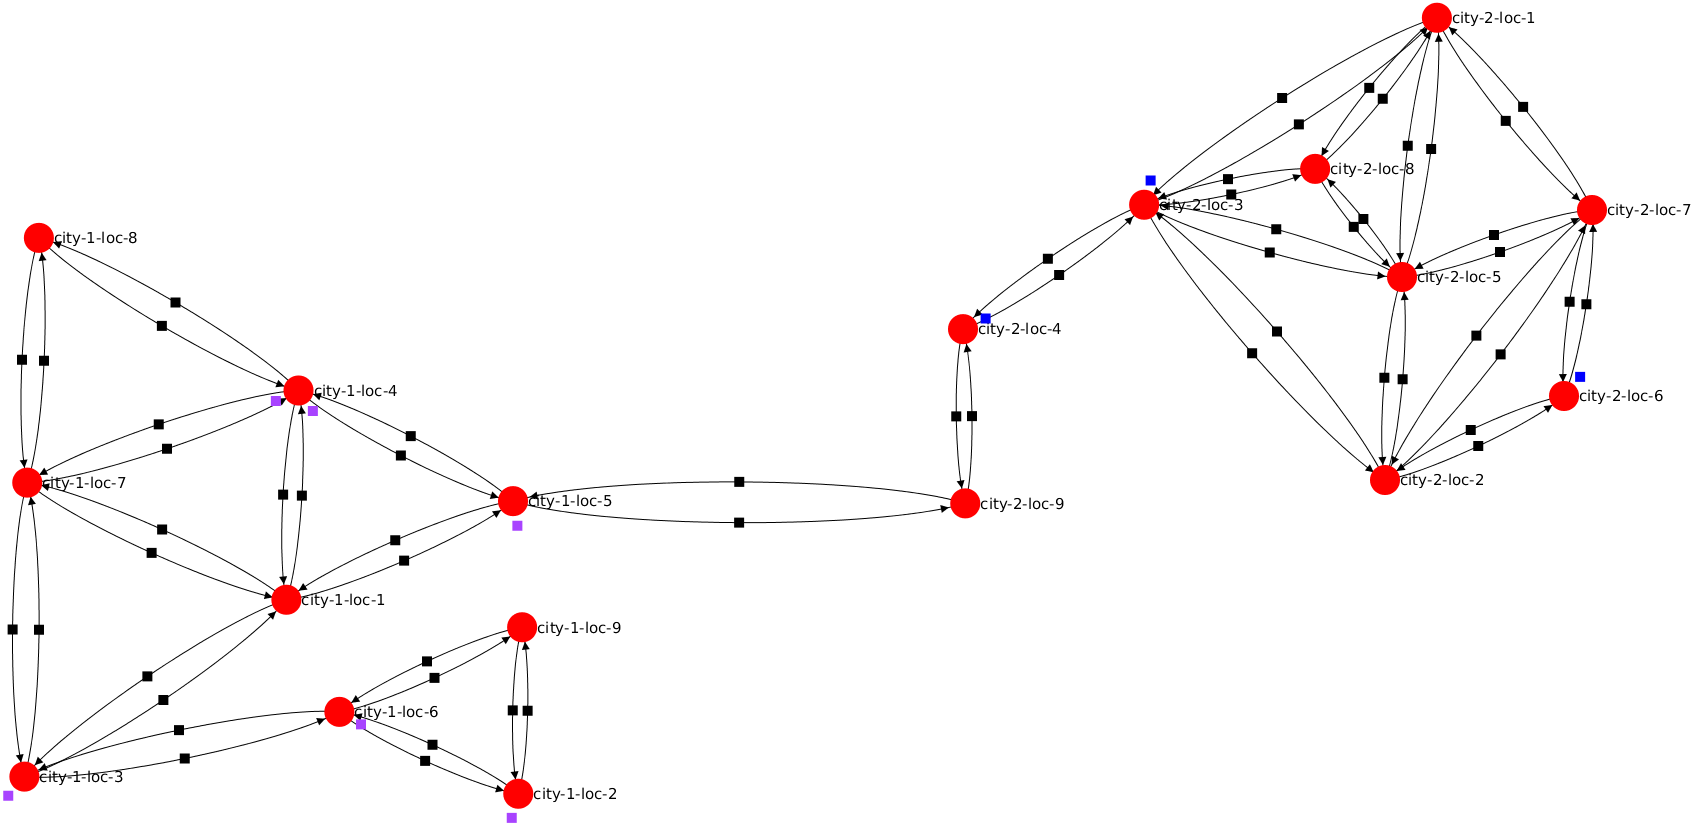
\includegraphics[width=1.0\textwidth]{../img/ipc08_seq-sat_p13_land2}
\end{center}
\caption[Visualization of the \texttt{p13} problem of sequential Transport from IPC 2008.]{Road graph visualization of the \texttt{p13} problem of the seq-sat track of IPC 2008. Red dots represent locations (graph nodes), roads (graph edges) are represented by black arrows, vehicles are plotted as blue squares, and packages as purple squares.}
\label{fig:ipc08_seq-sat_p13}
\end{figure}

\subsection{Transport Numeric}\label{transport-numeric}

The numeric variant adds the concept of fuel on top of the STRIPS variant.
All roads have an additional cost, called \verb+fuel-demand+, which is
subtracted from a vehicle's \verb+fuel-left+ value if it chooses to drive along that road.
Additionally, all vehicles have a maximum fuel capacity \verb+fuel-max+,
which they regain upon being the target of a \verb+refuel+ action. This action can only
be executed at a location that is marked as having a petrol station. Petrol stations
are static with respect to a given planning problem instance.

This variant is usually denoted as \textit{Transport numeric} or \textit{transport-numeric}.

\subsection{Transport Temporal}\label{transport-temporal}

The temporal Transport domain is usually denoted as \textit{Transport temporal} or, confusingly,
also \textit{transport-numeric}. A major difference with respect to the numeric variant is
the addition of time. All actions now have a duration (\verb+pick-up+ and \verb+drop+ both have a
duration of 1, \verb+refuel+ has a duration of 10, and the duration of \verb+drive+ is
equal to the length of the road we are driving along). Furthermore, packages can now have any integral size.

The addition of time poses numerous technical complications when formalizing this variant
--- its PDDL (Section~\ref{pddl}) formulation significantly differs from the two previous ones, but only in technical details, not in objectives of the model.
One important technicality is that a vehicle cannot pick up or drop packages concurrently --- it always handles packages one at a time. Also, vehicles cannot do other actions during driving to another location (they are essentially placed ``off the graph'' for the duration of driving).

The overall goal remains largely the same (deliver packages to their destinations), but we no longer optimize the total cost. Instead, we now minimize the total duration of a plan,
defined as the maximum time when an action is still taking place.
In practice, this translates to minimizing maximum end time over all actions, which is often referred to as minimizing the \textit{makespan}.



















\section{Formalizing the Transport domain}

We will now translate the informal description of the Transport domain from the previous section to the formal representations we defined in Section~\ref{classical-planning}. We will not formulate all the domain variants in all representations as
they are very much alike and not needed for the comprehension of the following chapters.

\subsection{Transport's classical representation}\label{transport-classical-representation}

We are now able to show the sequential Transport domain in one of the representations
previously defined, namely,
the classical representation (Figure~\ref{code:classical-strips}).
For practical reasons, we will use a slight modification, obtained by adding a limited concept of functions
with finite integer values.
It is obvious that we could substitute these functions for the appropriate relations
and a finite amount of literals for the numbers for any given problem instance of
the domain in this representation,
so that it adheres to the definition of a classical formulation.
For example, we could add literals representing a finite set of
natural numbers and a predicate that represents
a successor relation, defined as $\texttt{successor}(a, b) \equiv a + 1 = b$.

Note that this representation does not contain the notion of a \textit{total cost}
of a plan that we will optimize for later.
The predicates used are:
\begin{itemize}
\item \verb+at(o, l)+, the package or vehicle \verb+o+ is at the
location \verb+l+;
\item \verb+capacity(v, s)+, the vehicle \verb+v+ currently has \verb+s+ free space --- \verb+s+ is a variable for space literals, a set of literals denoting the amount of space (essentially,
these literals are a unary representation of a finite set of integers);
\item \verb+capacity-predecessor(s1, s2)+, the space literals represented by \verb+s1+ and \verb+s2+
satisfy the relation $\texttt{s1} + 1 = \texttt{s2}$
in the unary representation;
\item \verb+in(p, v)+, the package \verb+p+ is in the vehicle \verb+v+;
\item \verb+road(l1, l2)+, the location \verb+l1+ is directly adjacent to the location
\verb+l2+ by a road; and
\item \verb+road-length(l1, l2)+, the driving distance between location \verb+l1+
and \verb+l2+, modeled as a numerical function. Does not change while planning.
\end{itemize}

\begin{figure}[tbp]
\begin{code}
drive(v, l1, l2)
  ;; vehicle v moves from location l1 to an adjacent location l2
  precond: at(v, l1), road(l1, l2)
  effects: not at(v, l1), at(v, l2)

pick-up(v, l, p, s1, s2)
  ;; vehicle v picks up package p at location l,
  ;; decreasing its capacity from s2 to s1
  precond: at(v, l), at(p, l), capacity-predecessor(s1, s2),
           capacity(v, s2)
  effects: not at(p, l), in(p, v), capacity(v, s1),
           not capacity(v, s2)
  
drop(v, l, p, s1, s2)
  ;; vehicle v drops package p at location l,
  ;; increasing its capacity from s1 to s2
  precond: at(v, l), in(p, v), capacity-predecessor(s1, s2),
           capacity(v, s1)
  effects: not in(p, v), at(p, l), capacity(v, s2),
           not capacity(v, s1)
\end{code}
\caption{Classical formulation of \texttt{transport-strips}.}
\label{code:classical-strips}
\end{figure}

The numeric variant  adds the \verb+refuel+ operator, changes the \verb+drive+
operator, and adds a new fuel-related predicate \verb+has-petrol-station(l)+, that is true when the given location \verb+l+ has
a petrol station.
To model fuel, we need the addition of a few functions, namely:

\begin{itemize}
\item \verb+fuel-demand(l1, l2)+, the amount of fuel needed to drive
from location \verb+l1+ to location \verb+l2+;
\item \verb+fuel-left(v)+, the amount of fuel left in
the vehicle \verb+v+; and
\item \verb+fuel-max(v)+, the maximum amount of fuel
the vehicle \verb+v+ can contain, i.e. its fuel tank capacity.
\end{itemize}



We also abuse the notation with \verb+decrease+ and \verb+assign+;
the left parameter's value is to be decreased by the right
parameter's value or the left parameter's value is to be overridden
by the right parameter's value, respectively.

See Figure~\ref{code:classical-numeric} for the exact differences
in the representation after adding fuel.

\begin{figure}[tbp]
\begin{code}
drive(v, l1, l2)
  ;; vehicle v moves from location l1 to an adjacent location l2
  precond: at(v, l1), road(l1, l2), fuel-left(v) >= fuel-demand(l1, l2)
  effects: not at(v, l1), at(v, l2),
           decrease(fuel-left(v),  fuel-demand(l1, l2))
  
refuel(v, l)
  ;; vehicle v is refueled to the maximum at location l
  precond: at(v, l), has-petrol-station(l)
  effects: assign(fuel-left(v), fuel-max(v))
\end{code}
\caption[Partial classical formulation of \texttt{transport-numeric}.]{Classical formulation of \texttt{transport-numeric}'s differences compared to \texttt{transport-strips}.}
\label{code:classical-numeric}
\end{figure}

\subsection{Transport's state-variable representation}

We are now also able to show the sequential Transport domain
in the state-variable representation (Figure~\ref{code:statevar-strips}).
Some predicates (\verb+at+, \verb+capacity+ and \verb+in+) have been transformed
into state-variable functions with largely the same semantics as in
Section~\ref{transport-classical-representation}. Again, we leave out
the \textit{total cost} notion.

\begin{figure}[tbp]
\begin{code}
drive(v, l1, l2)
  ;; vehicle v moves from location l1 to an adjacent location l2
  precond: at(v) = l1, road(l1, l2)
  effects: at(v) <- l2

pick-up(v, l, p, s1, s2)
  ;; vehicle v picks up package p at location l,
  ;; decreasing its capacity from s2 to s1
  precond: at(v) = l, at(p) = l, s1 + 1 = s2, s2 > 0, capacity(v) = s2
  effects: at(p) <- nil, in(p) <- v, capacity(v) <- s1
  
drop(v, l, p, s1, s2)
  ;; vehicle v drops package p at location l,
  ;; increasing its capacity from s1 to s2
  precond: at(v) = l, in(p) = v, s1 = s2 - 1, capacity(v) = s1
  effects: in(p) <- nil, at(p) <- l, capacity(v) <- s2
\end{code}
\caption{State-variable formulation of \texttt{transport-strips}.}
\label{code:statevar-strips}
\end{figure}

The numeric variant again adds the \verb+refuel+ operator along with
a few fuel-related state-variable functions and predicates, and changes 
the \verb+drive+ operator (Figure~\ref{code:statevar-numeric}).

\begin{figure}[tb]
\begin{code}
drive(v, l1, l2)
  ;; vehicle v moves from location l1 to an adjacent location l2
  precond: at(v) = l1, road(l1, l2),
           fuel-left(v) >= fuel-demand(l1, l2)
  effects: at(v) <- l2, 
           fuel-left(v) <- fuel-left(v) - fuel-demand(l1, l2)
  
refuel(v, l)
  ;; vehicle v is refueled to the maximum at location l
  precond: at(v) = l, has-petrol-station(l)
  effects: fuel-left(v) <- fuel-max(v)
\end{code}
\caption[Partial state-variable formulation of \texttt{transport-numeric}.]{State-variable formulation of \texttt{transport-numeric}'s differences
compared to \texttt{transport-strips}.}
\label{code:statevar-numeric}
\end{figure}

We will represent the temporal variant of Transport using a variant of the state-variable representation using temporal planning operators, further referred to as the \textit{temporal state-variable representation}.
On top of the fuel-related predicates and functions from \verb+transport-numeric+, temporal Transport adds:
\begin{itemize}
\item \verb+package-size(p)+, a function with positive integer values representing the size of the package \verb+p+ (does not change during planning); and
\item \verb+ready-loading(v)+, a predicate used for ``locking'' the vehicle \verb+v+ during \pickup{} and \drop{} actions (enforcing the property of these two actions happening sequentially in time for a given vehicle). It is important to note that the \refuel{} action does not
lock the vehicle, which means the vehicle can be refueled while dropping off and picking up packages.
\end{itemize}
Figure~\ref{code:statevar-temporal} shows the temporal state-variable representation of Transport temporal, using a shorter but clear notation.
Note that both \pickup{} and \drop{} cancel the \verb+at+ predicate at the start of the action, which forbids parallel pickup and drop.

\begin{figure}[tb]
\begin{code}
drive(v, l1, l2)
  ;; vehicle v moves from location l1 to an adjacent location l2
  duration: road-length(l1, l2)
  cond: (at(v) = l1)@s, (road(l1, l2))@s,
        (fuel-left(v) >= fuel-demand(l1, l2))@s
  effects: (at(v) <- nil)@s, (at(v) <- l2)@e,
           (fuel-left(v) <- fuel-left(v) - fuel-demand(l1, l2))@s

pick-up(v, l, p)
  ;; vehicle v picks up package p at location l
  duration: 1
  cond: (at(v) = l1)@[s, e), (at(p) = l1)@s, (ready-loading(v))@s,
        (capacity(v) >= package-size(p))@s
  effects: (at(p) <- nil)@s, (in(p) <- v)@e, (not ready-loading(v))@s,
           (capacity(v) <- capacity(v) - package-size(p))@s,
           (ready-loading(v))@e
  
drop(v, l, p)
  ;; vehicle v drops package p at location l
  duration: 1
  cond: (at(v) = l1)@[s, e), (in(p) = v)@s, (ready-loading(v))@s
  effects: (in(p) <- nil)@s, (at(p) <- l)@e, (not ready-loading(v))@s,
           (capacity(v) <- capacity(v) + package-size(p))@e,
           (ready-loading(v))@e
  
refuel(v, l)
  ;; vehicle v is refueled to the maximum at location l
  duration: 10
  cond: (at(v) = l1)@[s, e), (has-petrol-station(l))@s
  effects: (fuel-left(v) <- fuel-max(v))@e
\end{code}
\caption[State-variable formulation of temporal Transport.]{Temporal state-variable formulation of temporal Transport. The characters \texttt{s} and \texttt{e} represent the start and end temporal variables of the given action, respectively.}
\label{code:statevar-temporal}
\end{figure}

\subsection{PDDL formulation of Transport}

All formulations of the Transport domain use PDDL (Section~\ref{pddl}) version 2.1,
with the requirement \verb+typing+, which adds the notion of types for individual
literals. We will call these literals \textit{action objects}.

The STRIPS variant additionally needs \verb+action-costs+, a requirement adding
integer costs to individual planning operators. These costs may be constant
(like the ones for \verb+pick-up+, \verb+drop+ or \verb+refuel+),
or they may be dependent on the parameters of the instantiated operator (like
the cost of \verb+drive+).
The numeric variant
requires \verb+numeric-fluents+, which introduces native PDDL support for functions whose values correspond to numbers and can change over time. It also requires are
\verb+goal-utilities+, used for custom optimization functions and optional goal predicates.
The temporal domain is similar in requirements to the numeric one, except for
substituting \verb+goal-utilities+ for \verb+durative-actions+ (introduces time
and the duration of actions).
For reference, we will now show the PDDL representation of the sequential and temporal variant of
the Transport domain in Figure~\ref{code:pddl-strips} and Figure~\ref{code:pddl-temporal} respectively.

\begin{figure}[tbp]
\begin{code}
(:action drive
  :parameters (?v - vehicle ?l1 ?l2 - location)
  :precondition (and
      (at ?v ?l1)
      (road ?l1 ?l2))
  :effect (and
      (not (at ?v ?l1))
      (at ?v ?l2)
      (increase (total-cost) (road-length ?l1 ?l2))))
(:action pick-up
  :parameters (?v - vehicle ?l - location ?p - package
               ?s1 ?s2 - capacity-number)
  :precondition (and
      (at ?v ?l)
      (at ?p ?l)
      (capacity-predecessor ?s1 ?s2)
      (capacity ?v ?s2))
  :effect (and
      (not (at ?p ?l))
      (in ?p ?v)
      (capacity ?v ?s1)
      (not (capacity ?v ?s2))
      (increase (total-cost) 1)))
(:action drop
  :parameters (?v - vehicle ?l - location ?p - package
               ?s1 ?s2 - capacity-number)
  :precondition (and
      (at ?v ?l)
      (in ?p ?v)
      (capacity-predecessor ?s1 ?s2)
      (capacity ?v ?s1))
  :effect (and
      (not (in ?p ?v))
      (at ?p ?l)
      (capacity ?v ?s2)
      (not (capacity ?v ?s1))
      (increase (total-cost) 1)))
\end{code}
\caption{Formulation of actions in PDDL for \texttt{transport-strips}.}
\label{code:pddl-strips}
\end{figure}

\begin{figure}[tbp]
\begin{code}
(:durative-action drive
  :parameters (?v - vehicle ?l1 ?l2 - location)
  :duration (= ?duration (road-length ?l1 ?l2))
  :condition (and
      (at start (at ?v ?l1))
      (at start (road ?l1 ?l2))
      (at start (>= (fuel-left ?v) (fuel-demand ?l1 ?l2))))
  :effect (and
      (at start (not (at ?v ?l1)))
      (at end (at ?v ?l2))
      (at start (decrease (fuel-left ?v) (fuel-demand ?l1 ?l2)))))
(:durative-action pick-up
  :parameters (?v - vehicle ?l - location ?p - package)
  :duration (= ?duration 1)
  :condition (and
      (at start (at ?v ?l))
      (over all (at ?v ?l))
      (at start (at ?p ?l))
      (at start (>= (capacity ?v) (package-size ?p)))
      (at start (ready-loading ?v)))
  :effect (and
      (at start (not (at ?p ?l)))
      (at end (in ?p ?v))
      (at start (decrease (capacity ?v) (package-size ?p)))
      (at start (not (ready-loading ?v))) ; lock vehicle
      (at end (ready-loading ?v)))) ; unlock vehicle
(:durative-action drop
  :parameters (?v - vehicle ?l - location ?p - package)
  :duration (= ?duration 1)
  :condition (and
      (at start (at ?v ?l))
      (over all (at ?v ?l))   
      (at start (in ?p ?v))
      (at start (ready-loading ?v)))
  :effect (and (at start (not (in ?p ?v)))
      (at end (at ?p ?l))
      (at end (increase (capacity ?v) (package-size ?p)))
      (at start (not (ready-loading ?v))) ; lock vehicle
      (at end (ready-loading ?v)))) ; unlock vehicle
(:durative-action refuel
  :parameters (?v - vehicle ?l - location)
  :duration (= ?duration 10)
  :condition (and
      (at start (at ?v ?l))
      (over all (at ?v ?l))
      (at start (has-petrol-station ?l)))
  :effect
      (at end (assign (fuel-left ?v) (fuel-max ?v))))
\end{code}
\caption{Formulation of durative actions in PDDL for temporal Transport.}
\label{code:pddl-temporal}
\end{figure}
















\section{Related problems}

To the best of our knowledge, there has been no attempt at producing domain-dependent planners
for Transport (IPC 2008, 2011, 2014 and unsolvability IPC 2016) or any other similar IPC domain, like Logistics (IPC 1998\comment{\footnote{\url{https://web.archive.org/web/20151017170331/http://ipc98.icaps-conference.org/}}} and 2000),
Depots (IPC 2002\comment{\footnote{\url{https://web.archive.org/web/20170408120817/http://ipc02.icaps-conference.org/domains.html}}}),
DriverLog (IPC 2002 and 2014),
or Trucks (IPC 2006).
All techniques we know of applied to Transport so far are the
domain-independent planners used in the three before-mentioned competitions.

Most of the research done on transportation-related problems and their automation
generally focuses
on a famous combinatorial optimization problem, the \textit{Traveling Salesman Problem} (TSP), on which an
exhaustive amount of research has been done \citep{Applegate1998, Applegate2011}. Its precise origins are unknown, but the problem has been on the minds of researchers at least since the end of the 19$^\textrm{th}$ century. The TSP is defined by \citet{Applegate2011} as follows:
\begin{quote}
Given a set of cities along with the cost of travel between each pair of them, the \textit{traveling salesman problem}, or \textit{TSP} for short, is to find the cheapest way of visiting all the cities and returning to the starting point. The ``way of visiting all the cities'' is simply the order in which the cities are visited; the ordering is called a \textit{tour} or \textit{circuit} through the cities.
\end{quote}
However, the problem we aim to study is more similar to a different optimization problem based on the TSP. See Figure~\ref{fig:tsp} for an illustrative example of a TSP solution.

\begin{figure}[tbp]
\begin{center}
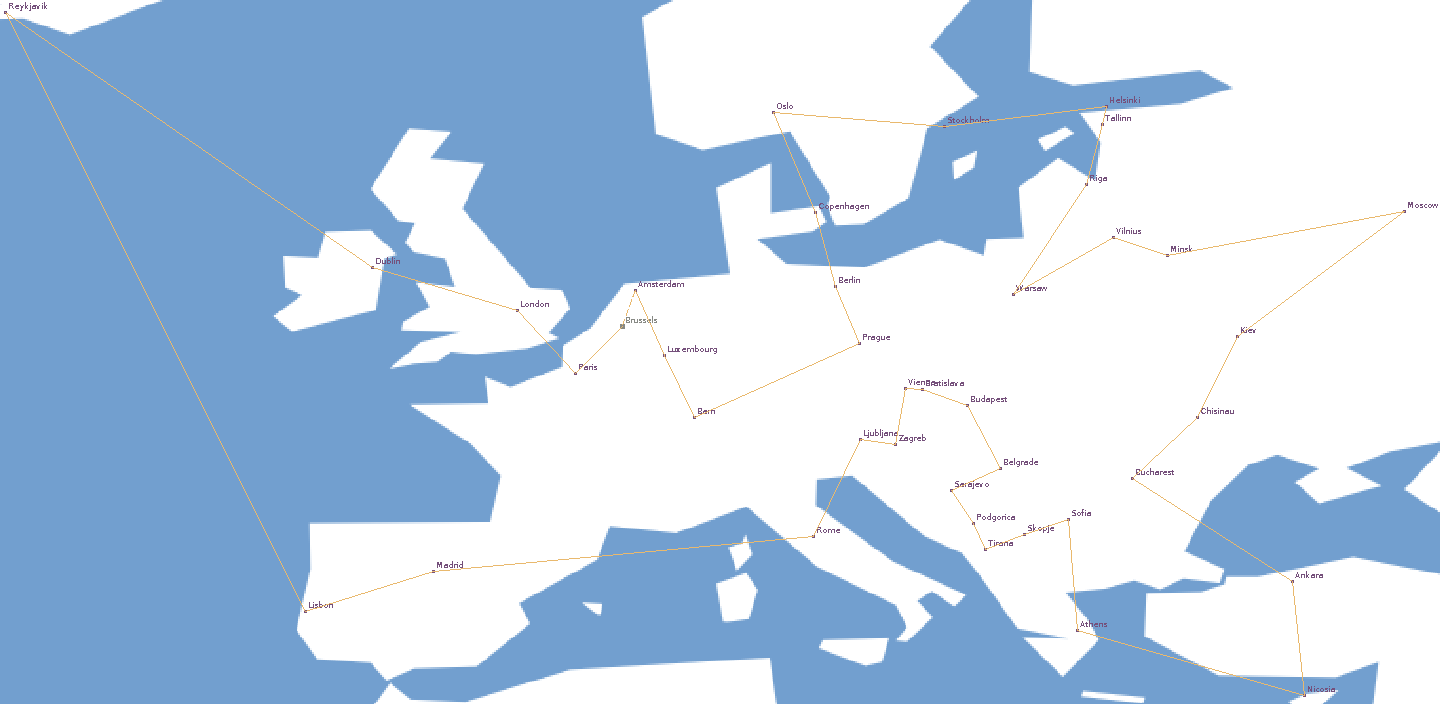
\includegraphics[width=1.0\textwidth]{../img/tsp}
\end{center}
\caption[An example TSP solution through the capitals of Europe.]{An example TSP solution through the capitals of Europe. Screenshot taken from OptaPlanner \citep{DeSmet2017}.}
\label{fig:tsp}
\end{figure}

\subsection{The Vehicle Routing Problem}\label{vrp}

The \textit{Vehicle Routing Problem} (VRP) was first formulated as the \textit{Truck Dispatching Problem} by \citet{Dantzig1959}, modeling a fleet of vehicles delivering gasoline to service stations. They described VRP
as a generalization of the TSP with multiple vehicles, but it could equivalently be stated that the TSP is a specialization of the VRP
with a single vehicle. The precise formulation of the Truck Dispatching Problem in \citep[Section~2]{Dantzig1959} represents a model with a fleet of identical vehicles departing from a single depot. According to \citet[Section~3]{Braekers2016}, this defines what we would call \textit{Capacitated VRP} (CVRP) today (Figure~\ref{fig:vrp}).

\begin{figure}[tbp]
\begin{center}
\includegraphics[width=0.7\textwidth]{../img/vrp}
\end{center}
\caption[An example CVRP solution for 32 customers and one depot.]{An example CVRP solution for 32 customers and one depot. Screenshot taken from OptaPlanner \citep{DeSmet2017}.}
\label{fig:vrp}
\end{figure}

Many VRP variants have emerged since. \citet{Eksioglu2009} and \citet{Braekers2016} both
review and classify hundreds of papers related to the VRP, with many more left out.
Most of these works tend to study the CVRP problem with minor modifications, hence creating
a broad landscape of problems and a platform to build on for the future.
According to the data in \citet[Table~4]{Braekers2016}, there has been a recent uptick
in popularity for models relatively similar to Transport --- specifically, VRPs with
backhauls (returning items from customers to depots),
multiple depots (multiple starting points for vehicles), and with allowed split deliveries (multiple
vehicles can serve a single customer).
The literature review on multiple depot VRP (MDVRP) in \citet{Montoya-Torres2015}
suggests a big rise in popularity for MDVRP in the recent past,
which provides further proof of relevance for studying the Transport domain.

Traditional solutions for the VRP include exact approaches like branch and bound
or constraint satisfaction
programming
that explore the large parts of the feasible search space,
classical heuristics which limit the search space, and also metaheuristics (general heuristics for devising specific heuristics), like genetic algorithms, local search, tabu search, and many more.

\comment{
\subsection{VRP Formulation}\citep{ResearchGroup2013}

The VRP is a combinatorial problem whose ground set is the edges of a graph ${G(V,E)}$. The notation used for this problem is as follows:

\begin{itemize}
\item ${V = \left\lbrace v_{0}, v_{1}, \ldots, v_{n} \right\rbrace}$ is a vertex set, where:
\begin{itemize}
\item Consider a depot to be located at ${v_0}$.
\item Let ${V' = V \backslash \left\lbrace v_{0} \right\rbrace}$ be used as the set of ${n}$ cities.
\end{itemize}
\item ${A = \left\lbrace(v_{i},v_{j}) | v_{i},v_{j} \in V; i \neq j \right\rbrace}$ is an arc set.
\item ${C}$ is a matrix of non-negative costs or distances ${c_{ij}}$ between customers ${v_{i}}$ and ${v_{j}}$.
\item ${d}$ is a vector of the customer demands.
\item ${R_{i}}$ is the route for vehicle ${i}$.
\item ${m}$ is the number of vehicles (all identical). One route is assigned to each vehicle.
\end{itemize}

When $c_{ij} = c_{ji}$ for all $(v_{i}, v_{j}) \in A$ the problem is said to be symmetric and it is then common to replace ${A}$ with the edge set $E = \lbrace (v_{i},v_{j}) | v_{i},v_{j} \in V; i < j \rbrace$.

With each vertex ${v_{i}}$ in ${V'}$ is associated a quantity ${q_{i}}$ of some goods to be delivered by a vehicle. The VRP thus consists of determining a set of ${m}$ vehicle routes of minimal total cost, starting and ending at a depot, such that every vertex in ${V'}$ is visited exactly once by one vehicle.

For easy computation, it can be defined ${b(V) = \left\lceil \sum_{v_{i} \in V} d_{i}) / C \right\rceil}$, an obvious lower bound on the number of trucks needed to service the customers in set ${V}$.

We will consider a service time $\delta_{i}$ (time needed to unload all goods), required by a vehicle to unload the quantity ${q_{i}}$ at ${v_{i}}$. It is required that the total duration of any vehicle route (travel plus service times) may not surpass a given bound ${D}$, so, in this context the cost ${c_{ij}}$ is taken to be the travel time between the cities. The VRP defined above is NP-hard [Lenstra \& Rinnooy Kan 1981].

A feasible solution is composed of:

\begin{itemize}
\item a partition ${R_{1}, \ldots, R_{m}}$ of ${V}$;
\item a permutation ${\sigma_{i}}$ of ${R_{i} \bigcup {0}}$ specifying the order of the customers on route ${i}$.
\end{itemize}


The cost of a given route (${R_{i} = \left\lbrace v_{0}, v_{1}, \ldots, v_{m+1} \right\rbrace}$), where ${v_{i} \in V}$ and ${v_{0} = v_{m+1} = 0}$ (0 denotes the depot), is given by ${C(R_{i}) = \sum_{i=0}^{m} c_{i,i+1} + \sum_{i=1}^{m} \delta_{i}}$.

A route ${R_{i}}$ is feasible if the vehicle stop exactly once in each customer and the total duration of the route does not exceed a prespecified bound ${D}$: ${C(R_{i}) \leq D}$.

Finally, the cost of the problem solution ${S}$ is: ${F_{VRP} = \sum_{i=1}^{m} F(R_{i})}$.
}

\subsection{Comparison of Transport and VRP}

In \citet{ResearchGroup2013}, a website was created, which serves as a comprehensive resource on the history of VRP,
definitions of its various flavors, and an overview of the popular solution methods and state-of-the-art results. According to the taxonomy they propose, we could characterize a Transport domain problem
as a \textit{Multiple Depot, Split Delivery, Capacitated VRP with Satellite Facilities}. Multiple Depot
means that vehicles can start driving from multiple locations, split delivery
means a single customer can be served by multiple vehicles, capacitated VRP adds maximum
capacities to vehicles, and satellite facilities mean that vehicles can pick items up
while on a delivery route. This does not characterize the Transport domain in every detail, but it is a fairly accurate approximation.

According to another VRP taxonomy and study of papers, presented in \citet{Eksioglu2009} and adapted in \citet{Braekers2016}, no research has been done on a VRP variant with a similar subset of features to those of Transport in any single study, to the best of our knowledge.
Usually, the studied problems are more constrained than Transport --- for example, they make additional assumptions about the places where vehicles start or end. Also, VRP in general
makes cooperation of vehicles hard to model, whereas in Transport this is one of the fundamental elements.

\comment{Transport could be characterized as \textit{2.1.1, 2.2.1, 2.4.1, 2.5.1, 2.8.1, 3.1.1, 3.2.2, 3.3.3, 3.4.2, 3.5.2, 3.7.1, 3.8.1, 3.9.3, 3.10.1, 3.11.1, 4.1.1, 4.2.1, 4.3.2, 4.4.1, 5.1.2.}}

An important difference between Transport and the VRP is that Transport has a notion of single packages or items. In the VRP, transported goods are usually regarded as measurable, rather than countable (for example gasoline or milk vs. letters or parcels). This makes a difference not only in the
interpretation, but also during problem-solving --- \textit{customers} in VRP usually request
a quantity of the delivered item, not specific item instances, like packages being ``requested''
by their target locations in Transport.

\chapter{Transport domain analysis}

In this chapter, we will analyze two variants of the Transport domain: sequential and temporal. To do this, we will describe a system we developed for the analysis
and development of planners for Transport, describe and analyze the datasets
used for devising experiments, and discuss the properties of Transport
that will help us in developing better quality planners.

\section{TransportEditor -- A Transportation Planning System}

To enable effective transportation planning,
we have developed \textit{TransportEditor}, a system for creating and visualizing transportation problems and plans.
Specifically, TransportEditor aims to be a problem editor and plan visualizer for the Transport domain (and its variants). It is an intuitive and cross-platform graphical desktop application (Figure~\ref{fig:transporteditor-screenshot})
written in Java.

It allows the user to create a planning session, where they
select a Transport domain variant, load a problem instance from PDDL (Section~\ref{pddl}) or create a new one from scratch.
The road network of the problem is automatically laid out and visualized for the user as a graph with locations as nodes and roads as edges.
Users can then tweak the layout, make changes to vehicle and package properties
and export the problem or domain back into PDDL.

They can also select an external planner
referencing its executable file, or select one of the built-in planners and try to solve
the loaded problem using the selected planner. Internal and external plan validators, like VAL \citep{Howey2003}, can also be selected to verify plans are correct.
Once plans are loaded and verified, it will let the user see a list of actions
in the plan, or plot a Gantt chart (useful for observing concurrent actions in temporal domain variants).

The best feature of TransportEditor is the option of tracing plans. We can select
any action, specify an exact time point or just step through the actions in order and
the road network on the left will display the current state of the problem, as if
all actions before the current point were applied to the start state.
It is possible to do all of this, and more, without ever leaving the TransportEditor user interface.

TransportEditor will help researchers working on this domain fine-tune their planners; they can visualize the various corner cases their planner fails to handle, step through the generated plan and find the points where their approach fails.
A secondary motivation is to be able to test approaches for creating plans for the domain.
For screenshots of typical TransportEditor usage, see the attached \nameref{transport-editor-screenshots}.

\begin{figure}[tbp]
\begin{center}
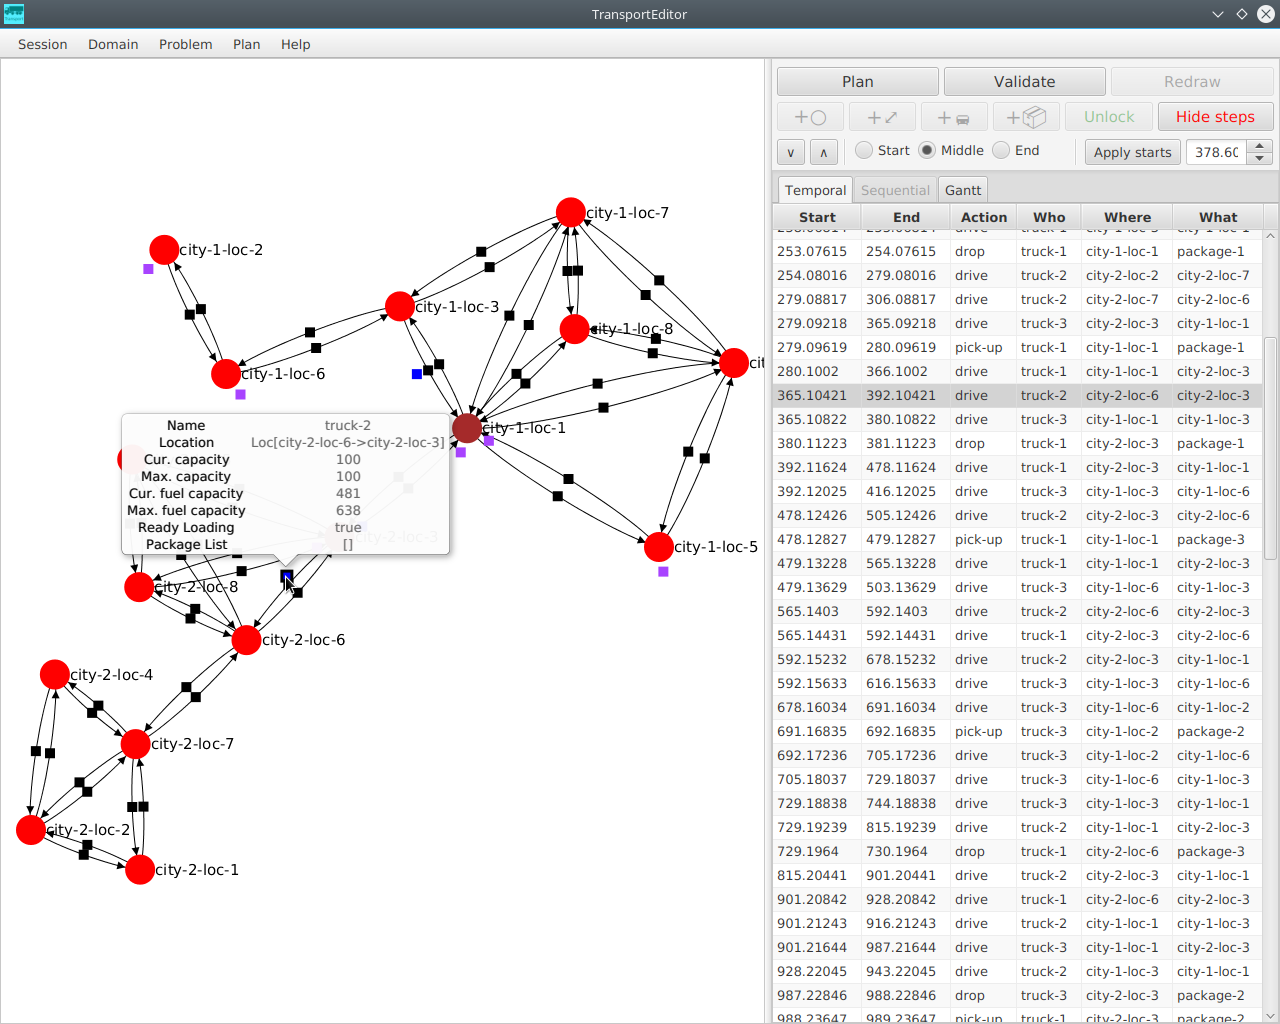
\includegraphics[width=0.9\textwidth]{../img/transporteditor_temporal}
\end{center}
\caption{Screenshot of a user tracing actions of a plan for a smaller temporal problem in TransportEditor.}
\label{fig:transporteditor-screenshot}
\end{figure}

The basic user workflow of TransportEditor consists of the following steps:
\begin{itemize}
\item Selecting which formulation of the Transport domain they want to work with or create their own variant;
\item Loading the PDDL or creating their own problem of the given domain. TransportEditor then visualizes the given graph as good as it can;
\item Iterating among the following options:
\begin{itemize}
\item Loading a planner executable and letting TransportEditor run the planner on the loaded problem instance for a given time (the user can cancel anytime),
then loading the resulting plan;
\item Possibly loading a pre-generated plan;
\item Stepping through the individual plan actions and letting TransportEditor visualize them.
The user can step forward and backward in the plan and inspect each action result in great detail;
\item Editing the graph: adding/removing/editing the location or properties of vehicles, packages, roads, locations and possibly petrol stations;
\item Saving the currently generated plan;
\item Saving the problem;
\item Saving the domain (exporting to a PDDL file).
\end{itemize}
\item Saving and closing the currently loaded problem. Exit the application or go back to the first step.
\end{itemize}

TransportEditor is a part of this thesis and you can find it on the attachment CD (see the attached \nameref{cd-contents} for more information). Both the \nameref{transporteditor-user-manual},
the \nameref{transporteditor-developer-manual}, and the \nameref{transporteditor-developer-javadoc} are attached to this thesis in a digital format, offering guidance when
using the program and providing an in-depth description.

















\section{Problem datasets}

For evaluation and comparison with other planners, we have acquired several problem datasets from previous runs of the IPC.
Table~\ref{tab:ipc-datasets} provides an overview of the individual datasets, their associated IPC competition, the track at the competition and the domain variant the problems are modeled in.

\begin{table}[tb]
\begin{tabular}{c||ccc}
\textbf{Dataset} & \textbf{Competition} & \textbf{IPC Track} & \textbf{Formulation} \\ 
\hline
\hline
netben-opt-6 & IPC-6 & \href{http://icaps-conference.org/ipc2008/deterministic/NetBenefitOptimization.html}{Net-benefit: optimal} & Numeric \\ 
seq-opt-6 & IPC-6 & \href{http://icaps-conference.org/ipc2008/deterministic/SequentialOptimization.html}{Sequential: optimal} & STRIPS \\ 
seq-sat-6 & IPC-6 & \href{http://icaps-conference.org/ipc2008/deterministic/SequentialSatisficing.html}{Sequential: satisficing} & STRIPS \\ 
tempo-sat-6 & IPC-6 & \href{http://icaps-conference.org/ipc2008/deterministic/TemporalSatisficing.html}{Temporal: satisficing} & Temporal \\ 
\hline
seq-agl-8 & IPC-8 & \href{https://helios.hud.ac.uk/scommv/IPC-14/seqagi.html}{Sequential: agile} & STRIPS \\ 
seq-mco-8 & IPC-8 & \href{https://helios.hud.ac.uk/scommv/IPC-14/seqmulti.html}{Sequential: multi-core} & STRIPS \\ 
seq-opt-8 & IPC-8 & \href{https://helios.hud.ac.uk/scommv/IPC-14/seqopt.html}{Sequential: optimal} & STRIPS \\ 
seq-sat-8 & IPC-8 & \href{https://helios.hud.ac.uk/scommv/IPC-14/seqsat.html}{Sequential: satisficing} & STRIPS \\ 
\end{tabular}
\caption{Transport datasets from the 2008 and 2014 IPCs.}
\label{tab:ipc-datasets}
\end{table}

Short descriptions of the various tracks and subtracks can be found in the rule pages of IPC-6\footnote{\url{http://icaps-conference.org/ipc2008/deterministic/CompetitionRules.html}}
and the rule pages of IPC-8\footnote{\url{https://helios.hud.ac.uk/scommv/IPC-14/rules.html}}.
Unfortunately, we weren't able to acquire the datasets for IPC-7 (2011), as the Subversion repository\footnote{\url{http://www.plg.inf.uc3m.es/ipc2011-deterministic/Domains.html}} that promises to contain them is unavailable.

We have decided to split our further research based on the tracks at IPC: we will focus on constructing
Transport-specific planners for the seq-sat-6, seq-sat-8, and tempo-sat-6 datasets.
Both the seq-sat-6 and tempo-sat-6 contain 30 problems, while seq-sat-8 only contains 20.
From the competition results, we have reasonable scores to compare our planners to.
Figure~\ref{fig:datasets-seq-sat} and Figure~\ref{fig:datasets-tempo-sat} show the
dimensions of each 


Truck goals: tempo-sat: 21-30



\TODO{specific problems we will be using, what we have chosen and why and how big they are}

\TODO{features and peculiarities of the problem instances}
















\section{Properties of Transport domains}

In this section, we will delve more deeply into the Transport domain and try to analyze its properties.
We will describe the problem instances that have been used in the IPC and discuss potential
heuristics and approaches to creating plans for these problems.



\subsection{Does domain knowledge make Transport easy to solve?}

When domain-independent planners solve a sequential Transport problem,
they face a harder task than our planners that have domain knowledge ahead of time.
Deciding whether a plan of a given length exists is, in the case of Transport,
an NEXPTIME-complete task \citep[Section~3.4]{Ghallab2004}.
That does not mean domain knowledge makes Transport easy. We will now show
that even the sequential variant of Transport is NP-hard.

\begin{thm}
The problem of finding an optimal plan for an undirected connected graph in the sequential
Transport domain is NP-hard. \TODO{Formulate better and revise proof}
\end{thm}
\begin{proof}
It is not evident if the problem is in NP: if we get a plan, there is no straightforward
way of verifying whether it is optimal.

We will now show that we can reduce an NP-complete problem to our problem in polynomial time,
hence proving that all NP-complete problems are reducible to our problem,
and therefore, our problem is NP-hard.

As proven by \citet{Karp1972}, the problem of existence of a Hamilton circuit (HC) in a (directed or undirected) graph is NP-complete. We will show that we are able to transform the HC problem into a sequential Transport problem.

Given an undirected graph $G$, the solution to HC is a cycle through all the nodes of $G$,
without visiting any single node twice.
We can use the same graph to model a Transport problem instance.
The problem will contain only one vehicle of capacity $n-1$,
where $n = |G|$, the number of nodes in the graph.

We will co-locate $n-1$ packages with the vehicle at any predetermined graph vertex $l \in G$.
One package $p'$ will be located elsewhere, at $l' \in G,\, l \neq l'$.
Each package positioned at $l$ will have a different target than the other packages at $l$
and none of the targets will be $l$. The package at $l'$ will have the original node $l$
as its target. We will set all road lengths to $1$. 

An optimal plan for the designed translation has a total cost of at least $3n$.
Any plan for this problem has to have at least $n$ \verb+drive+ actions, because
there is a package to be delivered to every node, and the graph has $n$ nodes.
Because it has to move $n$ packages, at least $n$ \verb+pick-up+ and $n$ \verb+drop+
actions are needed. The costs of all actions are 1.
We conjecture that an HC exists if and only if an optimal and valid plan visits each vertex only once.

First, we prove the forward implication. Assume an HC exists and the optimal plan visits at least one node twice. We can now construct a plan with a lower total cost than the optimal plan: first, pick up all the $n-1$ co-located packages, then drive along the HC. At each
visited node, drop the package that has this node as its destination. If we are at $l'$,
pick up the package $p'$. The plan is trivially valid, as it delivers all packages
and the vehicle never over-reaches its capacity. Also, its total cost is $3n$
(the length of the HC is $n$, which implies $n$ drive actions) and for every of the $n$ packages, we do exactly one \verb+pick-up+ and exactly one \verb+drop+. Hence, the plan
is optimal and visits each vertex only once.

Now, assume an HC does not exist. If the found optimal plan only visits each node once,
we can look at the source locations of all \verb+drive+ actions and the target
location of the last \verb+drive+ action. They constitute a path through the graph on which a node never repeats and the path starts and finishes at the same node.
Hence, we have constructed a HC.
\end{proof}

\subsection{Sequential variant properties}

\TODO{insights, degenerate cases, etc.}


\subsection{Temporal variant properties}

\TODO{insights, degenerate cases, etc.}
















\section{Original competition results}

\TODO{re-read and refactor after moving here}

In the updated results of the seq-sat track of IPC 2008\footnote{\url{http://icaps-conference.org/ipc2008/deterministic/Results.html}} published after the competition,
the overall winner \textit{lama} (a Fast-Downward \TODO{ref} planner configuration)
was hands-down the best planner on the sequential Transport domain, winning
with a total quality of $28.93/30$, where all other planners had less than $20/30$.
Only 5 problem instances were solved suboptimally by \textit{lama}.
\textit{Quality} is calculated for a given planner and problem $p$
as $$\frac{\mt{total-cost}(\mt{planner}(p))}{\mt{total-cost}(BEST)},$$ where the results called $BEST$
are precalculated outside of the competition environment, or the best result of a planner in the competition, depending on which plan has a lower total cost. The quality is, therefore, a number between $0$ and $1$. The total quality is calculated as the sum of qualities on all problem instances.

As mentioned, we were not able to gather data from the IPC 2011,
hence the results cannot be meaningfully interpreted.
The competition featured 20 sequential Transport problems,
with 4 planners achieving a total quality of more than $15/20$.

In the seq-sat track of IPC 2014, the winner on the Transport domain
was without a doubt the \textit{Mercury} planner, achieving
a stunning $20/20$ total quality. Even more interesting is the fact that
the runner-up \textit{yahsp3-mt} achieved a score of $10.74/20$
and all other planners achieved sub $10/20$ total quality.
The IPC 2014 used different problem instances than the IPC 2008
and we will test our approaches on both datasets.

The temporal variant of Transport was only used in IPC 2008.
Planners that entered that competition did not cope well with the domain
--- only two non-baseline planners were able to produce at least one plan
for any problem. Additionally, only the simple problem (\verb+p01+) was solved
optimally by any planner. The best total quality was only $7.5/30$, achieved by
\textit{sgplan6}. No other domain in the temporal track had a lower best total quality
than Transport, which, assuming reasonably generated problem instances, hints
at Transport being one of the harder domains for domain-independent temporal planners.

\TODO{expand into subsections and try to analyze why}
















\section{Accompanying software toolkit architecture}

\TODO{Modules, classes, what belongs where, etc}


















\section{Formulating Transport as a CSP}\label{csp-formulation}

\TODO{intro}

\subsection{Na{\"{i}}ve formulation}

We will now formulate a sequential Transport (Section~\ref{transport-strips}) problem as a CSP (Section~\ref{csp}) using the na{\"{i}}ve encoding provided in \citet[Section~8.3]{Ghallab2004}.
However, using that strategy, our problems ``blow up'' in size --- as is expected due
to the different complexities of planning versus solving CSPs \citep[Section~8.3.2]{Ghallab2004}. To visualize the difference in our case, we have constructed a state space estimation table (Table~\ref{tab:csp-trivial}) for conversions of two sample sequential Transport problems.

\begin{table}[tb]
\begin{center}
\begin{tabular}{l||rr}
\textbf{Features / estimates} & \textbf{p01} & \textbf{p20} \\ 
\hline 
\hline 
\textbf{Best known plan length} & 6 & 351 \\ 
\textbf{Vehicles} & 2 & 4 \\ 
\textbf{Vehicle variables} & 14 & 1 408 \\ 
\textbf{Packages} & 2 & 20 \\ 
\textbf{Package variables} & 14 & 7 040 \\ 
\textbf{Locations} & 5 & 60 \\ 
\textbf{Roads} & 12 & 256 \\
\textbf{Max capacity} & 4 & 4 \\ 
\hline
\textbf{Ground Drive actions} & 168 & 360 448 \\ 
\textbf{Ground PickUp actions} & 140 & 1 689 600 \\ 
\textbf{Ground Drop actions} & 140 & 1 689 600 \\ 
\hline 
\textbf{Planning variables total} & 48 & 10 207 \\ 
\textbf{Grounded actions total} & 448 & 1 189 838 848 \\ 
\textbf{Search Space Estimate} & $\approx 1.1 \cdot 10^{52}$ & $\approx 1.4 \cdot 10^{27 952}$ \\ % https://www.wolframalpha.com/input/?i=(245120%5E351)+*+4%5E1408+*+60%5E1408+*+1468%5E7040
\end{tabular}
\end{center}
\caption[Search space approximations for a na{\"{i}}ve CSP encoding.]{CSP Search space approximations for the \textit{p01} and \textit{p20} problems from the \textit{seq-sat} track of IPC 2008, using the general and domain-independent encoding from \citet[Section~8.3]{Ghallab2004}.}
\label{tab:csp-trivial}
\end{table}

The first section of the table (rows 1--7) contains problem-specific constants.
The two calculated values in that section, \textit{Vehicle variables} and \textit{Package variables} are the amounts of variables generated for the respective
object by grounding it for every intermediate plan state (before and after applying an action). Therefore, the value is equal to the number of vehicles/packages of the problem
multiplied by the set plan length $+ 1$ (each state corresponds to the state before applying an action + the last state).

In the second section (rows 8--10), we estimate the number of ground actions
Step 1 from \citet[Section~8.3.1]{Ghallab2004} will generate.
We calculate the number of \pickup{} and \drop{} actions the CSP encoding will generate
as $$(\mt{length(plan)} + 1) \cdot \mt{\#vehicles} \cdot \mt{\#locations} \cdot \mt{\#packages},$$
effectively counting all ground planning operators of the problem. Similarly,
the number of \drive{} actions is calculated as
$$(\mt{length(plan)} + 1) \cdot \mt{\#vehicles} \cdot \mt{\#roads},$$
which is more efficient than the na{\"{i}}ve way of
counting all
$$(\mt{length(plan)} + 1) \cdot \mt{\#vehicles} \cdot \mt{\#locations}^2$$
actions.

As we can see from the third section of the table, the number of variables
(planning variables and ground actions) is not extremely high
--- the problem is that the variables have very large domains,
which makes the CSP problem exponentially larger \citep[Section~8.3.2]{Ghallab2004}.
We calculated the \textit{Search Space Size Estimate} (SSE) as
\begin{align*}
\mt{SSE} =\; &\mt{\#ground\_actions}^{l-1} & \textit{\footnotesize select ground actions for the plan}\\
&\cdot \mt{\#capacities}^{l \cdot \mt{\#vehicles}} & \textit{\footnotesize select capacities for vehicle variables}\\
&\cdot \mt{\#locations}^{l \cdot \mt{\#vehicles}} & \textit{\footnotesize select locations for vehicle variables}\\
&\cdot (\mt{\#locations} + \mt{\#vehicles})^{l \cdot \mt{\#pkg}}, & \textit{\footnotesize select locations/vehicles for package variables}
\end{align*}
where we set $l := \mt{length(plan) + 1}$.
For comparison to the SSEs in the last table row, 
the estimated number of atoms in the universe is generally estimated to be about $4 \cdot 10^{80}$.

\subsection{Domain-dependent formulation}\label{csp-custom-repr}

\TODO{domain-dep formulation, note the shadow variable overhead}
\TODO{New cap represents advantages: memory while keeping the same expressive power. Reduction only in state vars}


\begin{table}[tb]
\begin{center}
\begin{tabular}{l||rr}
\textbf{Features / estimates} & \textbf{p01} & \textbf{p20} \\ 
\hline 
\hline 
\textbf{Best known plan length} & 6 & 351 \\ 
\textbf{Vehicles} & 2 & 4 \\ 
\textbf{Vehicle shadow vars} & 14 & 1 408 \\
\textbf{Packages} & 2 & 20 \\ 
\textbf{Package shadow vars} & 14 & 7 040 \\
\textbf{Locations} & 5 & 60 \\ 
\textbf{Roads} & 12 & 256 \\
\textbf{Max capacity} & 4 & 4 \\ 
\hline
\textbf{Ground Drive actions} & 24 & 1024 \\ 
\textbf{Ground PickUp actions} & 20 & 4800 \\ 
\textbf{Ground Drop actions} & 20 & 4800 \\ 
\hline 
\textbf{Planning variables total} & 48 & 10 207 \\ 
\textbf{Grounded actions in step} & 64 & 10 624 \\ 
\textbf{Action type orderings} & 2 187 & $\approx 8.8 \cdot 10^{167}$ \\ 
\textbf{Search Space Estimate} & $\approx 1.5 \cdot 10^{14}$ & $\approx 2.0 \cdot 10^{637}$ \\
\end{tabular}
\end{center}
\caption[Search space approximations for a domain-dependent CSP encoding.]{CSP Search space approximations for the \textit{p01} and \textit{p20} problems from the \textit{seq-sat} track of IPC 2008, using a custom domain-dependent CSP encoding for Transport sequential.}
\label{tab:csp-custom}
\end{table}

Using the domain-dependent encoding specified previously, we are now able to construct
a search space estimate table for the same Transport problems (Table~\ref{tab:csp-custom}). While the table rows look similar, sections 2 and 3 are calculated
differently. The ground action counts in section 2 are not multiplied by $\mt{length(plan)} + 1$
as done previously, because we only represent them once, not at every plan state.
The total number of grounded actions is the same, but they are not explicitly represented as variables. The Search Space size Estimate is therefore calculated differently:
\begin{align*}
\mt{SSE} =\; &3^{\mt{length(plan)} + 1} & \textit{\footnotesize select the action type of each action}\\
&\cdot \mt{\#ground\_actions}^{l-1}. & \textit{\footnotesize select the specific ground action}
\end{align*}
For comparison to the na{\"{i}}ve encoding SSEs which going from the p01 problem to the p20 grow by a logarithmic factor of approximately $538$,
whereas the domain-dependent ones only grow by approximately $46$,
which is a huge improvement.

Given the search space reduction, we will attempt to use this representation
for constructing a CSP-based planner in Section~\ref{csp-approach}.

\chapter{Sequential Transport planning}

In this chapter, we describe the planning approaches we
selected, implemented, and tested for the STRIPS variant of Transport.
Throughout this, we will leverage the acquired
Transport domain knowledge as much as possible.

\section{State-space forward planning}\label{forward-planning}

One of the most straightforward approaches to automated planning
is forward search \citep[Section~4.2]{Ghallab2004}
in state space (Figure~\ref{alg:forward-search}).
Although the algorithm is defined on a classical representation,
it can be used on any planning problem, where we can:
\begin{itemize}
\item determine whether a state is a goal state or not;
\item iterate over all actions applicable to a state; and
\item compute a successor state by applying an action to the current state.
\end{itemize}
Forward search, despite its simplicity, is one of the most frequently
used approaches for domain-independent planners.
There are two key steps of the algorithm, which
cause the most problems in practice: representing
the applicable actions (step 6) and choosing the
next action to apply (step 8).

\myalg{Forward Search}%
{%
\Input a planning problem in a classical representation $\mathcal{P} = (S, O, \gamma, s_0, g)$
\Output a plan $\pi$
\Function{Forward-Search}{$\mathcal{P}$}
\State $s \gets s_0$
\State $\pi \gets $ empty plan
\Loop
\If {$s$ satisfies $g$} \Return $\pi$ \EndIf
\State $A_s \gets \{a \,|\, o \in O$, $a$ is a ground instance of $o \;\&\; \mt{precond}(a) \mt{ is true in } s\}$
\If {$A_s = \emptyset$} \Return failure \EndIf
\State (nondeterministically) choose an action $a \in A_s$
\State $s \gets \gamma(s, a)$
\State $\pi \gets$ append $a$ to $\pi$
\EndLoop
\EndFunction
}%
{A forward search planning algorithm.}{A forward search planning algorithm for Transport. Adapted from \citet[Figure~4.1]{Ghallab2004}.}{forward-search}{bt}

Representing state transitions in step 6
is a technical problem of representing successor states
in state space search \citep[Section~3.2]{Russell1995}.
Due to limited memory,
applicable actions are grounded from operators
on demand, as are the corresponding successor states
\citep[Section~3.4]{Russell1995}.

The forward search algorithm, in its specified form, is nondeterministic.
If we knew which action to choose in step 8,
we would know how to solve the planning problem.
Since we generally do not know which action (state transition) to chose in a given state, the choice is usually delegated to a suitable
search algorithm, which makes forward search deterministic.


\subsection{Deterministic search algorithms}

State space search algorithms are a heavily studied area
of computer science and any reasonable search algorithm applied
to forward search will yield results.
Examples of such algorithms are Breadth-First Search (BFS),
Depth-First Search (DFS), and many more \citep[Section~3.5]{Russell1995}.
The choice of a search algorithm greatly influences
the quality of resulting plans when applied to forward search.

As sizes of planning problems grow,
choosing a search algorithm is even more crucial.
Several well-performing algorithms on small problems (like BFS)
exceed reasonable run times and become unusable for practical application on larger problems.
An important and practically useful search algorithm
withstanding larger problem sizes is the \textit{A$^{\kern-.05em*}$ algorithm} (Figure~\ref{alg:astar})
introduced in \citet{Hart1968}.

\myalg{Forward Search with A$^{\kern-.15em*}$}%
{%
\Input a classical planning problem $\mathcal{P} = (S, O, \gamma, s_0, g)$,
a heuristic $h$
\Output a plan $\pi$
\Function{Collect-Plan}{$s, \pi$}
\State $\pi' \gets $ empty list
\While{$s \neq \emptyset$}
	\State $(s', a) \gets \pi[s]$
	\State $\pi' \gets$ prepend $a$ to $\pi'$
	\State $s \gets s'$
\EndWhile
\State \Return $\pi'$
\EndFunction

\Function{Forward-Search-Astar}{$\mathcal{P}$}
\State $\pi \gets $ empty map, $f[*] \gets \infty$, $g[*] \gets \infty$, $o \gets \{s_0\}$, $c \gets \emptyset$
\State $\pi[s_0] \gets \emptyset$,
$g[s_0] \gets 0$, $f[s_0] \gets h(s_0)$
\While{$o \neq \emptyset$}
\State $s \gets \mt{argmin}_{s' \in o} f[s']$, $o \gets o \setminus \{s\}$, $c \gets c \cup \{s\}$
\If {$s$ satisfies $g$} \Return \Call{Collect-Plan}{$s$, $\pi$} \EndIf
\ForAll{actions $a \in$ \Call{Generate-Actions}{$s, \pi$}}
	\State $s_n \gets \gamma(s, a)$ \Comment{Neighbor state}
	\If{$s_n \notin c$} \Comment{Not visited yet}
		\If{$s_n \notin o$} $o \gets o \cup \{s_n\}$ \Comment{Discovered a new state} \EndIf
		\If{$g[s] + \mt{cost}(a) < g[s_n]$} \Comment{Found a better path}
			\State $\pi[s_n] \gets (s, a)$
			\State $g[s_n] \gets g[s] + \mt{cost}(a)$
			\State $f[s_n] \gets g[s_n] + h(s_n)$
		\EndIf
	\EndIf
\EndFor
\EndWhile
\Return failure
\EndFunction
}%
{A forward search planning algorithm using A$^{\kern-.15em*}{\kern-.30em.}$}{A forward search planning algorithm using A$^{\kern-.15em*}{\kern-.30em.}$
\textsc{Generate-Actions} is a function that produces actions applicable to the state $s$. The notation $x[*] \gets y$  reprensents initialization of all values of the map $x$ to $y$.}{astar}{tb}

A$^{\kern-.15em*}$ has many important properties. We pinpoint one important to us, namely its admissibility.
A search algorithm is \textit{admissible}
if it is guaranteed to find an optimal path from a state $s$
to a goal state $s_g$ for any state space \citep{Hart1968}.
A$^{\kern-.15em*}$ is admissible and optimal given an admissible heuristic.

An \textit{admissible} heuristic never overestimates
the true value it is approximating. During planning in state space,
when examining a state $s$, we want to estimate the total cost of the best
plan that gets us to a goal state from state $s$. In other words, because we are
trying to minimize the total cost,
a planning heuristic $h: S \to \N_0$ is admissible if and only if $\forall s \in S : h(s) \leq h^*(s),$
where $h^*$ is the true total cost (i.e.\;the optimal heuristic). A similar definition is applicable for minimizing makespan in the temporal variant.

Furthermore, some heuristics have the property of being consistent. A heuristic $h$ is consistent
if and only if $\forall s \in S : h(s) \leq cost(a) + h(s_n)$
(where $a \in A : \gamma(s, a) = s_n$) and for all goal states $s_g$, it holds that $h(s_g) = 0$.
Consistent heuristics are sometimes called monotonic, because their value
does not increase along the best path to a goal state. Additionally,
it can be proven that consistent heuristics are always admissible
\citep[Section~4.1]{Russell1995}.



A slight modification of A$^{\kern-.15em*}{\kern-.30em,}$ called \textit{Weighted A$^{\kern-.05em*}$} \citep{Pohl1970},
tends to yield good quality plans in a shorter amount of time,
at the expense of
sacrificing admissibility. The only difference
when compared to A$^{\kern-.15em*}$ is that the heuristic $h(x)$
is substituted for $h_w(x) = w \cdot h(x),$
where $w \in \N_0$ is a weight constant. Choosing a weight greater
than 1 makes the heuristic inadmissible,
but guides the search towards a goal state faster.


\subsection{Heuristics for forward search in Transport}\label{seq-heuristics}

When designing a heuristic, we want to provide an estimate
of the total plan cost or makespan
that is as precise as possible, which
will help guide the search to a goal state as quickly as
possible.

We will now describe several heuristics for sequential
Transport using the state-variable representation.
In the following, the value of the $\mt{target(p)}$ function represents
the target location of a package $p$ in the set of packages $P$.

\subsubsection{Trivially admissible Transport heuristic}\label{sfa0}

The simplest domain-specific heuristic (apart from the zero heuristic $h_0 \equiv 0$) that is applicable to all variants of Transport
is one that counts the minimum number of \pickup{} and \drop{} actions
necessary to reach a goal state.
To obtain the correct count, we add 1 for each
package that is not yet at its destination (it will need to be dropped there) and another 1 for each package
that is, additionally, not in a vehicle (it will need to be picked up):

$$h'_{0}(s) = \sum_{\substack{
p \in P\\ \mt{at}(p) \neq \mt{target}(p)}} 1
+ \sum_{\substack{
p \in P\\ \mt{at}(p) \neq \mt{target}(p)\\
\mt{at}(p) \neq \mt{nil}}} 1.$$

The heuristic $h'_0$ is admissible, but it is practically unusable, as it
very poorly approximates
the cost of the optimal remaining actions to a goal state
--- recall that costs of \drive{} actions are generally much higher than the costs of \pickup{} and \drop{} actions.

\subsubsection{Package distance heuristic}\label{sfa1}

In \texttt{transport-strips}, the only thing we want is to deliver packages to their destinations. Therefore, a straightforward heuristic is one that calculates the length of a shortest
path of each package to its destination and sums the lengths for all packages.
To make the heuristic more precise, we can add the
value of $h'_0$ to it, as the \pickup{} and \drop{}
actions also have to occur in the optimal plan:
$$h_1(s) = h'_0(s) + \sum_{p \in P} \mt{spd}(location(p), target(p)),$$
where the $location: P \to L$ function,
with values in the set of all locations $L$, is defined as:
$$location(p) = \begin{cases}
   \mt{at}(p), & \text{if } \mt{at}(p) \neq \mt{nil},\\
   \mt{at}(\mt{in}(p)), & \text{else}.
  \end{cases}$$
The location of a package is, therefore, defined
as the location it is at, or, if it is loaded in a vehicle,
the location of the vehicle.
The function $\mt{spd}: L \times L \to \N_0$ represents
the shortest path distance between the two locations.

This heuristic is definitely not optimal, meaning that there are states,
where we will need to add actions to reach a goal state with a higher total cost than the value of the heuristic in that state.

However, it is important to note, the heuristic
is not even admissible, so its value might sometimes overestimate the total cost needed.
To see why, let us consider a network with just two locations $A$ and $B$.
A vehicle of capacity 2 and two packages are located at $A$ and both packages want to be
transported to $B$. The road between $A$ and $B$ is symmetric and has length
of a 1. It is trivial to see that the optimal plan consists of two \pickup{} actions,
followed by a \drive{} and two \drop{} actions. This plan has a total cost of $2+1+2=5$,
but the heuristic would estimate that we need actions
that cost $6$.

\subsubsection{Minimum spanning tree marking heuristic}\label{sfa2}

A different extension of the $h'_0$ heuristic
is the heuristic $h_2$ defined below, based
on finding the shortest paths on a \textit{minimum spanning tree} (MST).
Using an MST calculated using the algorithm presented in \citet{Kruskal1956}, we can solve one of the largest problems with $h_1$,
namely that we count an excessive amount of \drive{} actions
for packages to their targets.
For each package, we calculate
shortest path distances only on the MST.
Also, we do not calculate any edge twice --- we mark
the edge when it is part of a used shortest path and
after marking edges of all shortest paths,
we sum the lengths of the marked edges.
In the same way as with $h_1$, we add the value of $h'_0$ to
the sum.

Do note that this heuristic is yet again inadmissible:
let the road network be a circle of $n$ locations with
roads of lengths $1, 2, \ldots, n$ assigned clockwise.
An MST on this network consists of all roads except the road
with length $n$, let us denote the road $r = (A, B) \in L^2$.
Now, assume there is a package located at $A$ with a target
location of $B$ and a vehicle also located at $A$.
The optimal plan is obviously to pick up the package at $A$,
drive along road $r$ to $B$, and drop the package there.
The plan has a cost of $n+2$. The $h_2$ heuristic's estimate
in the initial state is:
$$h_2(s_0) = 2 + \sum_{i=1}^{n-1} i = \frac{n^2}{2} - \frac{n}{2} + 2,$$
which is evidently greater than $n+2$ for $n > 3$.

\subsubsection{Package and vehicle distance heuristic}\label{sfa3}

As an extension of the package distance heuristic,
we will also add the distance of the nearest vehicle for
each package:
$$h_3(s) = h_1(s) + \sum_{p \in P} \min_{v \in V} \mt{spd}(location(p), \mt{at}(v)),$$
where $V$ is the set of all vehicles.
As follows from the inadmissibility of $h_1$, $h_3$
is also inadmissible and nonoptimal.

\subsubsection{Package or vehicle distance heuristic}\label{sfa4}

A variation on the package and distance heuristic
is one that does not sum the shortest path distances, but instead takes
the minimum.
Specifically, for each package, the minimum
is taken from the distance to its target location,
distance to the nearest vehicle,
and the distance to the nearest package:
\begin{align*}
h_4(s) = h'_0(s) + \sum_{p \in P} \min\lbrace
&\mt{spd}(location(p), target(p)),
\min_{v \in V} \mt{spd}(location(p), \mt{at}(v)),\\
&\min_{\substack{p' \in P\\p' \neq p}} \mt{spd}(location(p), location(p'))\rbrace.
\end{align*}
We will now show the admissibility of this heuristic.
\begin{thm}
The heuristic $h_4$ is admissible for sequential Transport problems.
\end{thm}
\begin{proof}
Let $s$ be a state such that $h_4(s) > h^*(s)$,
where $h^*$ is a function of the real distance to the nearest goal state.
State $s$ is not a goal state, because for all goal states $s'$
it holds that
$h_4(s') = 0 = h^*(s'),$ due to all packages being at their target locations.
Let $s_g$ be the nearest goal state to $s$.

Because $h_4(s) > h^*(s)$, there exists a finite plan $\pi$ from the initial state $s$ that ends in $s_g$,
such that the total cost of $\pi$ is equal to $h^*(s)$.
Let $h^{(p)}_4(s)$ denote the value of a package's term in the sum of $h_4(s)$,
ignoring the contribution of $h'_0$.
Let $p \in P$ be any package that is not yet at its destination,
not loaded in a vehicle, and not at a location with any other packages
(all of those have $h^{(p)}_4(s) = 0$).

In the plan $\pi$, $p$ had to be delivered.
That means a vehicle (possibly more)
had to arrive at the
package's location, pick it up, drive it somewhere else and drop it,
possibly several times.
However, any vehicle could not have arrived at $p$'s current location from a location that is closer than: $$\min\{\min_{v \in V} \mt{spd}(location(p), \mt{at}(v)),
\min_{\substack{p' \in P\\p' \neq p}} \mt{spd}(location(p), location(p'))\} \leq h^{(p)}_4(s),$$
and at least one vehicle had to arrive at the package's location.
The \pickup{} and \drop{} actions for each package have to be planned in $\pi$ as well, at least in the corresponding counts that $h'_0$ adds.

This means, that $\pi$ had to have actions that correspond at least to the costs of:
$$h'_0(s) + \sum_{p \in P} h_4^{(p)}(s) = h_4(s),$$
which implies $h_4(s) \leq cost(\pi) = h^*(s),$ and that is a contradiction.
\end{proof}

Despite its admissibility, the $h_4$ heuristic is not consistent. Let us assume the following road network (Figure~\ref{fig:heursit}):
$$\{\{A, B, 1\}, \{B, C, 2\}, \{B, D, 2\}\},$$
where $\mt{at}(v) = A$, $\mt{at}(p_1) = C,$ and $\mt{at}(p_2) = D$
hold in the initial state $s_0$.
The target of $p_1$ is $D$ and the target of $p_2$ is $C$.
The value:
$$h_4(s_0) = 3+3+4 = 10$$ is greater than the cost
of the applicable \drive{} action for vehicle $v$ from $A$ to $B$
added to the heuristic value in the updated state:
$$cost(a) + h_4(s') = 1 + (2+2+4) = 9.$$
The heuristic is also not optimal, as is evident from the same
example situation (for $s_0$, the optimal plan is of length $13$).

\begin{figure}[b]
\centering
\begin{subfigure}{0.48\textwidth}
\centering
\includegraphics[width=0.75\textwidth]{../imga/heursit}
\caption{Counterexample for $h_4$.}
\label{fig:heursit}
\end{subfigure}
\begin{subfigure}{0.48\textwidth}
\centering
\includegraphics[width=0.75\textwidth]{../imga/heursit_h5}
\caption{Counterexample for $h_5$.}
\label{fig:heursit_h5}
\end{subfigure}
\caption{Visualization of the counterexample road networks
for consistency of heuristics $h_4$ and $h_5$.}
\label{fig:heursits}
\end{figure}

\subsubsection{General marking heuristic}\label{sfa5}

The heuristic $h_5$ is a generalization of the MST marking heuristic $h_2$. We calculate $h_5$ in the exact same way by marking roads,
except for
using an MST --- instead, the whole graph is used.
We also mark roads on the shortest path from each package to the nearest
vehicle or package or target location, depending on which is nearer (similar
to the package or vehicle distance heuristic).
Shortest path ties are broken arbitrarily.
Do note that if a package is loaded in a vehicle, no roads are marked for it.

The described heuristic is not optimal, but it is admissible.
Both properties hold because $\forall s \in S : h_5(s) \leq h_4(s)$ holds
and they hold for $h_4$.

Even though $h_5$ is consistent in far more situations (combinations of states and applicable actions) than $h_4$, it is still not consistent in general.
Assume the following road network (Figure~\ref{fig:heursit_h5}):
$$\{\{A, B, 1\}, \{A, C, 1\}, \{A, D, 1\}, \{B, C, 2\}, \{B, E, 10\}, \{C, D, 2\}, \{D, E, 10\}\},$$
where $\mt{at}(v) = C$, $\mt{at}(p_1) = B,$ and $\mt{at}(p_2) = D$
hold in the initial state $s_0$.
The target of both $p_1$ and $p_2$ is $E$.
If the heuristic selects the red edges for $s_0$, the value:
$$h_5(s_0) = 2+2+4 = 8$$ is greater than the cost
of the applicable \drive{} action for vehicle $v$ from $C$ to $A$
added to the heuristic value in the updated state (assuming selection of blue edges):
$$cost(a) + h_5(s') = 1 + (1+1+4) = 7.$$
Note that the $h_5$ heuristic could have likewise selected the blue edges along
with the $\{A, C, 1\}$ edge, which would have resulted in $h_5(s_0) = 7,$
and this case would not be a counterexample. This points to the possibility that th $h_5$ heuristic will work reasonably ``consistenly'' in practice.

\subsubsection{Summary}

In our tests, we found that
the heuristics $h_0$, $h'_0$, $h_1$, and $h_2$
were too simple for practical usage.
The $h_3$ heuristic, while having no significant
theoretical properties performs surprisingly well in practice.
The $h_4$ heuristic on the other hand, while being admissible, does not
perform well empirically.
Due to its closeness to consistency, the $h_5$ heuristic has the best properties out of all the discussed heuristics and also
performs well in practice.
We will include planners utilizing the $h_3$ and $h_5$ heuristics
in our final evaluation (Chapter~\ref{experiments}).








\subsection{Sequential Forward A*}\label{sfa}

\textit{Sequential Forward A$^{\kern-.05em*}$} (SFA) is a planner for sequential Transport based on forward search using A$^{\kern-.15em*}$ (Figure~\ref{alg:astar}).
It utilizes most of the domain knowledge described
in Section~\ref{domain-info} and~\ref{datasets}
to prune the search space as much as possible
without sacrificing admissibility.

However, domain knowledge alone does not
prune away enough search space to
generate plans efficiently.
With the addition of
heuristics
from Section~\ref{seq-heuristics},
implementations of the planner become reasonably useful
on practical problems, as will be demonstrated
later during experimental evaluation.

A variant of SFA,
\textit{Weighted Sequential Forward A$^{\kern-.05em*}$} (WSFA)
swaps A$^{\kern-.15em*}$ search for Weighted A$^{\kern-.15em*}$ in the SFA planner.

\subsection{Meta-heuristically weighted SFA*}\label{msfa}

\textit{Meta-heuristically weighted SFA$^{\kern-.05em*}$} (MSFA) is
a meta-planner built on top of a WSFA planner with
a given heuristic.

Given two hyperparameters $\alpha \in [0, 1]$ and $w_0 \in [1, \infty)$,
it runs the WSFA planner with the weight $w \gets w_0$,
waits for the planner to find a plan,
and then (exponentially) decays the
weight of the heuristic function
with a minimum at 1: $$w \gets \max(1, \floor*{\alpha \cdot w}).$$

Do note that this is followed up by a complete restart of the internal WSFA planner.
If only a recalculation of values in the $f$ map
of forward search with A$^{\kern-.15em*}$ was done, all successive
weight runs would almost immediately return, because we are in the vincinity of a goal state,
but not necessarily the nearest one to the initial state.
In some sense, this simulates a quick DFS run followed up
by local search around the path found by DFS.
Generally, better results are obtained by reexploring the
state space from the initial state with an updated weight.

Even though this meta-planning approach breaks
admissibility guarantees, it works very well on
practical problems, even the larger ones.



















\section{Ad-hoc planning}\label{ad-hoc}

An approach that domain-independent planners by definition cannot utilize
is ad-hoc planning. We propose several
ad-hoc planners that generate decent quality plans very fast,
although they are usually suboptimal.
This becomes an advantage mainly when dealing with very large
problems or time-constrained planning,
like in the agile track of IPC.

\subsection{Randomized Restart Planning}\label{rand-restart}

We will now describe a family of planners which we will refer to as \textit{Randomized Restart} planners.
Each of these planners essentially performs the same algorithm (Figure~\ref{alg:rand-restart}),
with minor tweaks. The motivation
behind the algorithm is that the ``hardest'' part of Transport planning
is choosing where to drive with what vehicle.

\myalg{Randomized Restart planning}%
{%
\Input a Transport problem in a classical representation $\mathcal{P} = (S, O, \gamma, s_0, g)$
\Output a plan $\pi$
\Function{Randomized-Restart}{$\mathcal{P}$}
\State $\pi \gets $ empty plan, $\Pi \gets \infty$
\While{cancel not requested} \Comment{Canceled by an external request}
\State $s \gets s_0$, $\pi' \gets $ empty plan
\While{$s$ doesn't satisfy $g \And score(\pi') < \Pi$}
\State $A \gets $ \Call{Generate-Drive-Sequence}{$s$}
\ForAll{action $a \in A$} \Comment{Apply all actions to the state}
\State $s \gets \gamma(s, a)$
\EndFor
\If{$s = \emptyset$} \textbf{break} \Comment{At least one $a \in A$ was not applicable}
\EndIf
\State $\pi' \gets $ append all $a \in A$ to $\pi'$
\EndWhile
\If{$s$ satisfies $g \And score(\pi') < \Pi$}
\State $\pi \gets \pi'$, $\Pi \gets score(\pi')$ \Comment{Update the best plan}
\EndIf
\EndWhile
\State \Return $\pi$
\EndFunction
}%
{A Randomized Restart planning algorithm.}{A Randomized Restart planning algorithm. The \textsc{Generate-Drive-Sequence} function
generates a partial plan beginning in state $s$.
The exact definition of the function
depends on the specific algorithm variant as described in Section~\ref{rand-restart}.}{rand-restart}{tb}

The algorithm essentially does domain-dependent plan space planning
by iteratively adding sequences of \drive{} actions
intertwined with \pickup{} and \drop{} actions
until all packages are delivered.
To do all of this at speed, the vehicle used for the given sequence
is usually chosen randomly, as are the packages that are picked up and dropped along the driving path.
The biggest advantage, however, is gained by precomputing
a matrix of shortest paths and always using those to drive to the
selected locations.

Our randomized restart planners will generate many suboptimal plans,
but by always keeping a copy of the so far best found plan,
we can prune away the current partial plan if it becomes
worse than the best plan after adding a sequence.
Afterwards, we simply restart
from the initial state and iteratively generate a new candidate plan.
We utilize domain knowledge in all the planners,
for example by not picking up packages that are at their destination,
and using most of the other insights discussed in Section~\ref{domain-info}.

\subsubsection{Randomized Restart From Location Planner}\label{rrfl}

In each iteration of the before mentioned algorithm,
the Randomized Restart From Location planner (RRFL)
randomly chooses a vehicle and a location.
It adds \drive{} actions along the shortest path
to that location and greedily picks up as many packages as
its capacity allows.
It then calculates the optimal
path through all the picked up package target locations,
by trying the shortest paths through all possible permutations
of the locations.
Finally, it adds the appropriate \drive{} and \drop{} actions.

\subsubsection{Randomized Restart On Path Planner}\label{rrop}

The Randomized Restart On Path planner (RROP),
randomly chooses a vehicle
and a package that fits into the vehicle.
It then calculates the shortest path from the vehicle
to the package
and the shortest path from the package to its target location.
Afterwards, it finds all packages that have current and target locations on the path, taking into account the direction of driving.
It then tries all combinations of
those packages that do not make the vehicle become
overcapacitated over the whole course
of the path, in order
to find the combination that maximizes the minimum
free capacity over the course of the path.
If there are several such combinations, it minimizes the
maximum package drop location index in the path.
If there are still several combinations, it chooses one arbitrarily.
Finally, it adds the appropriate \drive{} and \drop{} actions.

\subsubsection{Randomized Restart On Path Nearby Planner}\label{rropn}

The Randomized Restart On Path Nearby planner (RROPN)
is a slight modification of RROP.
It first chooses a package randomly and then,
based on a probability $\varepsilon \in [0, 1]$,
either chooses a random vehicle that the package fits into,
or the nearest such vehicle.
The rest of the algorithm is identical to RROP.
The probability $\varepsilon$ is a hyperparameter,
which in our experiments is fixed to $0.2$,
which means that the probability of selecting the nearest vehicle is 80\%.

\subsubsection{Randomized Restart Around Path Nearby Planner}\label{rrapn}

Another randomized restart planner that is built on top of RROPN,
is the Randomized Restart Around Path Nearby planner (RRAPN).
It uses the same vehicle and package selection,
but it changes the way packages on the path are chosen to be loaded
onto the vehicle.

We still load as many packages that are completely on the path
as possible, using the same selection mechanism as in RROPN.
Additionally, for each package we precalculate
the location on the path that is closest to its target,
limited to locations after the package was picked up
in the correct driving direction.
Finally, we plan the \pickup{} and \drop{} actions of the
packages that greedily fit into the vehicle and
have the smallest precalculated distance to their target.

\subsubsection{Randomized Backtrack Around Path Nearby Planner}\label{rbapn}

We also developed a backtracking variant of RRAPN
called Randomized Backtrack Around Path Nearby (RBAPN).
Instead of choosing random vehicles and packages
it backtracks over the choices it makes,
guaranteeing to find an optimal
plan in the subspace of plans
generated by adding such action sequences as described in
the section about RRAPN. This approach is very
time-consuming and not practically usable.

\subsubsection{Randomized Restart Around Path Distribution Planner}\label{rrapd}

Another variant of RRAPN, the
Randomized Restart Around Path Distribution planner (RRAPD),
changes the vehicle choice inherited from RROPN.
Instead of using a biased coin flip based on the $\varepsilon$
hyperparameter, RRAPD samples the vehicle
from a discrete probability distribution
obtained by applying the \textit{softmax} function on the inverse distances of vehicles to the selected package:
\begin{align*}
\varphi'_i &= \frac{1}{\mt{spd}(location(p), \mt{at}(v_i)) + 1},\\
\varphi_i &= \frac{\exp(\varphi'_i/T)}{\sum_{j = 1}^{|V|} \exp(\varphi'_j/T)}.
\end{align*}
The value $\varphi_i$ is the resulting probability of each vehicle $v_i \in V = \{v_1, v_2, \ldots, v_n\}$.
The hyperparameter $T \in (0, \infty)$ is the \textit{temperature}
of the softmax. If set to higher values than 1, it
evens out the distribution --- higher probabilities shrink
and smaller probabilities become larger.
As $T$ grows large, the distribution will resemble a uniform distribution.
If $T$ is set to lower values, the distribution will prefer larger values.
In our experiments, we used a fixed $T = 0.1$, to prefer the nearest vehicles.

\subsubsection{Summary}

The implementations
of RRFL, RROP, and RROPN have empirically shown
lesser performance in our tests than RRAPN and RRAPD.
RRAPD, however, performs worse than RRAPN on
average.
As mentioned previously, RBAPN is unusable on larger
problems due to catastrophic run time in practice.
We will evaluate the Nearby planner
of the Randomized Restart Around Path
kind in our experiments in Chapter~\ref{experiments},
as they produce good quality plans in a very short time
even for larger problem instances.

All planners of the Randomized Restart family
are suboptimal, not only meaning that they sometimes produce
suboptimal plans, but also that for some problems,
even the best plan they can produce will be suboptimal.
This is easiest to prove for each planner individually,
by constructing a counterexample for a corner
case of the
greedy
choices
the planners make.



























\comment{
\section{Formulating Transport as a CSP}\label{csp-approach}

When discussing related works, we mentioned the Vehicle Routing Problem (Section~\ref{vrp}) and its straightforward
formulation as a Constraint Satisfaction Problem. Utilizing CSPs has been useful
for planning in the past \citep[Section~8.7]{Ghallab2004}
and we will attempt to use domain-specific knowledge to improve upon the standard, domain-independent
formulation.

\subsection{Na{\"{i}}ve CSP formulation}

We will now formulate a sequential Transport (Section~\ref{transport-strips}) problem as a CSP (Section~\ref{csp}) using the na{\"{i}}ve encoding provided in \citet[Section~8.3]{Ghallab2004}.


TODO{explain the model + constraints}


However, using that strategy, our problems ``blow up'' in size --- as is expected due
to the different complexities of planning versus solving CSPs \citep[Section~8.3.2]{Ghallab2004}. To visualize the difference in our case, we have constructed a state space estimation table (Table~\ref{tab:csp-trivial}) for conversions of two sample sequential Transport problems.

TODO{recalculate + verify numbers}

\begin{table}[tb]
\begin{center}
\begin{tabular}{l||rr}
\textbf{Features / estimates} & \textbf{p01} & \textbf{p20} \\
\midrule
\midrule
\textbf{Best-known plan length} & 6 & 351 \\
\textbf{Vehicles} & 2 & 4 \\
\textbf{Vehicle variables} & 14 & 1 408 \\
\textbf{Packages} & 2 & 20 \\
\textbf{Package variables} & 14 & 7 040 \\
\textbf{Locations} & 5 & 60 \\
\textbf{Roads} & 12 & 256 \\
\textbf{Max capacity} & 4 & 4 \\
\midrule
\textbf{Ground Drive actions} & 168 & 360 448 \\
\textbf{Ground PickUp actions} & 140 & 1 689 600 \\
\textbf{Ground Drop actions} & 140 & 1 689 600 \\
\midrule
\textbf{Planning variables total} & 48 & 10 207 \\
\textbf{Grounded actions total} & 448 & 1 189 838 848 \\
\textbf{Search Space Estimate} & $\approx 1.1 \cdot 10^{52}$ & $\approx 1.4 \cdot 10^{27 952}$ \\ % https://www.wolframalpha.com/input/?i=(245120%5E351)+*+4%5E1408+*+60%5E1408+*+1468%5E7040
\end{tabular}
\end{center}
\caption[Search space approximations for a na{\"{i}}ve CSP encoding.]{CSP Search space approximations for the \textit{p01} and \textit{p20} problems from the \textit{seq-sat} track of IPC 2008, using the general and domain-independent encoding from \citet[Section~8.3]{Ghallab2004}.}
\label{tab:csp-trivial}
\end{table}

The first section of the table (rows 1--7) contains problem-specific constants.
The two calculated values in that section, \textit{Vehicle variables} and \textit{Package variables} are the numbers of variables generated for the respective
object by grounding it for every intermediate plan state (before and after applying an action). Therefore, the value is equal to the number of vehicles/packages of the problem
multiplied by the set plan length + 1 (each state corresponds to the state before applying an action + the last state).

In the second section (rows 8--10), we estimate the number of ground actions
Step 1 from \citet[Section~8.3.1]{Ghallab2004} will generate.
We calculate the number of \pickup{} and \drop{} actions the CSP encoding will generate
as $$(\mt{length(plan)} + 1) \cdot \mt{\#vehicles} \cdot \mt{\#locations} \cdot \mt{\#packages},$$
effectively counting all ground planning operators of the problem. Similarly,
the number of \drive{} actions is calculated as
$$(\mt{length(plan)} + 1) \cdot \mt{\#vehicles} \cdot \mt{\#roads},$$
which is more efficient than the na{\"{i}}ve way of
counting all
$$(\mt{length(plan)} + 1) \cdot \mt{\#vehicles} \cdot \mt{\#locations}^2$$
actions.

As we can see from the third section of the table, the number of variables
(planning variables and ground actions) is not extremely high
--- the problem is that the variables have very large domains,
which makes the CSP problem exponentially larger \citep[Section~8.3.2]{Ghallab2004}.
We calculated the \textit{Search Space Size Estimate} (SSE) as
\begin{align*}
\mt{SSE} =\; &\mt{\#ground\_actions}^{l-1} & \textit{\footnotesize select ground actions for the plan}\\
&\cdot \mt{\#capacities}^{l \cdot \mt{\#vehicles}} & \textit{\footnotesize select capacities for vehicle variables}\\
&\cdot \mt{\#locations}^{l \cdot \mt{\#vehicles}} & \textit{\footnotesize select locations for vehicle variables}\\
&\cdot (\mt{\#locations} + \mt{\#vehicles})^{l \cdot \mt{\#pkg}}, & \textit{\footnotesize select locations/vehicles for package variables}
\end{align*}
where we set $l := \mt{length(plan) + 1}$.
For comparison to the SSEs in the last table row,
the estimated number of atoms in the universe is generally estimated to be about $4 \cdot 10^{80}$.

\subsection{Domain-dependent CSP representation}\label{csp-custom-repr}

We will now devise a different CSP representation for sequential Transport.
While not improving upon the search space estimates of the na{\"{i}}ve formulation
in a theoretical sense, we will describe a slightly more complex
and less general
CSP model that enables us to explore fewer states.

Using OptaPlanner and its shadow variable concept \citep[Section~4.3.6]{DeSmet2017}, we will model our Transport problem without keeping explicit track of capacities,
vehicle and package locations, and ground actions, all of which will be implicitly managed by OptaPlanner, or inferred in the case of capacity and actions.
This means we will reduce the memory overhead, maintaining the same expressive power
and hopefully not enlarge the processing time too much.

TODO{Describe the specific representation after it is polished in the code}

TODO{recalculate + verify numbers}

\begin{table}[tb]
\begin{center}
\begin{tabular}{l||rr}
\textbf{Features / estimates} & \textbf{p01} & \textbf{p20} \\
\midrule
\midrule
\textbf{Best-known plan length} & 6 & 351 \\
\textbf{Vehicles} & 2 & 4 \\
\textbf{Vehicle shadow vars} & 14 & 1 408 \\
\textbf{Packages} & 2 & 20 \\
\textbf{Package shadow vars} & 14 & 7 040 \\
\textbf{Locations} & 5 & 60 \\
\textbf{Roads} & 12 & 256 \\
\textbf{Max capacity} & 4 & 4 \\
\midrule
\textbf{Ground Drive actions} & 24 & 1024 \\
\textbf{Ground PickUp actions} & 20 & 4800 \\
\textbf{Ground Drop actions} & 20 & 4800 \\
\midrule
\textbf{Planning variables total} & 48 & 10 207 \\
\textbf{Grounded actions in step} & 64 & 10 624 \\
\textbf{Action type orderings} & 2 187 & $\approx 8.8 \cdot 10^{167}$ \\
\textbf{Search Space Estimate} & $\approx 1.5 \cdot 10^{14}$ & $\approx 2.0 \cdot 10^{637}$ \\
\end{tabular}
\end{center}
\caption[Search space approximations for a domain-dependent CSP representation.]{CSP Search space approximations for the \textit{p01} and \textit{p20} problems from the \textit{seq-sat} track of IPC 2008, using a custom domain-dependent CSP representation for Transport sequential.}
\label{tab:csp-custom}
\end{table}

Using the domain-dependent representation specified, we are now able to construct
a search space estimate table for the same Transport problems (Table~\ref{tab:csp-custom}).
Do note, that this table cannot be compared directly to the previous one,
because it hides the shadow variable management overhead.
Also, while the table rows look similar, sections 2 and 3 are calculated
differently. The ground action counts in section 2 are not multiplied by $\mt{length(plan)} + 1$
as done previously, because we only represent them once, not at every plan state.
The total number of grounded actions is the same, but they are not explicitly represented as variables. The Search Space size Estimate is therefore calculated differently:
\begin{align*}
\mt{SSE} =\; &3^{\mt{length(plan)} + 1} & \textit{\footnotesize select the action type of each action}\\
&\cdot \mt{\#ground\_actions}^{l-1}. & \textit{\footnotesize select the specific ground action}
\end{align*}
For comparison to the na{\"{i}}ve encoding SSEs which going from the p01 problem to p20 grow by a logarithmic factor of approximately $538$,
whereas the domain-dependent ones only grow by approximately $46$,
which is a huge improvement.

Given the search space reduction, we will now attempt to use this representation
for constructing a CSP-based planner.

\subsection{CSP-based planner}\label{csp-planner}

TODO{try to run a CSP in OptaPlanner to solve this and compare results, using Section~\ref{csp-custom-repr}}

TODO{Advantages and shortcommings of a CSP-based planner}

}
\chapter{Temporal transportation planning}

\section{Specifics of temporal planning}

\TODO{mention that there are vehicle goals.. verify!}

\section{Shortcommings of domain-independent approaches}

\TODO{Vytiahnut si plany z vysledkov seq-sat08 TFD a sgplan6, najst deficiencies}

\section{Interleaving actions of sequential plans}

\TODO{describe the idea of parallelizing sequential plans using ``mutexes''}

\TODO{easy to implement, leveraging existing work + describe shortcommings}

\section{A different temporal approach?}

\TODO{???}

\section{CSP-based temporal planner???}\label{csp-temporal-approach}

\TODO{only if sequential is good, or even then?}

\section{Summary and possible future approaches}

\TODO{Mention which planners we choose to compare in the experimental part}

\TODO{more possible approaches}

\chapter{Experimental evaluation}\label{experiments}

In this chapter, we will describe and run experiments
that compare our planners from the last two chapters
with domain-independent planners from the IPC.
We will briefly discuss the acquired results and interpret them.

\section{Methodology}

Using our benchmarking software (described in the attachments), we will now run experiments in an
environment similar to the original
IPCs. The rule pages state that
planners have to be single-threaded and use a maximum of 2, 4, or 6 GB of memory (depending on the competition year), with a maximum run time of 30 minutes.

Since the IPC rule pages vary on the exact processor specification or the amount of memory available to each planner between competitions,
we adjust the parameters slightly by only running our planners
for 15 minutes on each problem, using 4 GB of RAM.
All our experiments are run on
\comment{a computer
with an 8 core 64-bit processor \texttt{Intel Core i7-6700 CPU @ 3.40GHz}
and 16 GB of memory, running Gentoo Linux.
A big thank you goes out to the faculty for providing access to these machines.
}
the clusters of MetaCentrum.\puncfootnote{\url{https://www.metacentrum.cz/en/}}
Due to the nature of computing on MetaCentrum, we were not able to guarantee that all problems and planners
run on the exact same processor, only on very similar ones
(approximately equivalent to \texttt{Intel Xeon E5-2650 v2 2.6 GHz}).
The performance of our planners does not change significantly
when prolonging the run from 15 to 30 minutes or when run
on slightly different processors.
Our planners will get canceled and prompted for a plan after the 15 minutes run out. 

We run all our planner implementations in Java using Oracle's OpenJDK 
version \texttt{1.8.0\_131}.
The results presented here were obtained with the \TEver{} version of the TransportEditor project.\puncfootnote{Git tag \TEtag{}, available at \url{https://github.com/oskopek/TransportEditor}} The \texttt{NOTICE.txt} files
in the project module directories specify
the exact versions of libraries used.
In all planners where nondeterminism occurs,
we set the initial random seed to 2017
(on all individual problem runs).

The evaluation criteria remain the same as in the IPC:
we focus on plan \textit{quality} in favor of planner run time.
The quality of a plan for a specific planner and sequential problem $p$ is defined as:
$$\frac{\mt{total-cost}(\mt{planner}(p))}{\mt{total-cost}(BEST)},$$
where the results called $BEST$
are either precalculated outside of the competition environment or they are the best result of one of the planners in the competition, depending on which plan has a lower total cost.
Quality is, therefore, a number between $0$ and $1$.
The overall goal for planners is to maximize the sum of qualities over the problem instances in a given dataset, called the \textit{total quality}.
For temporal domains, quality is calculated in the same way, just by substituting total cost
for total time. We sometimes refer to total cost and total time as the \textit{score} of the planner, a term that is not dependent on the domain variant.

We will use four datasets for our experiments --- the seq-sat-6, seq-sat-7,
and seq-sat-8 datasets for sequential
and the tempo-sat-6 for temporal planners (Section~\ref{datasets}).
All the datasets used are available in the
software project sources (see the attached \nameref{cd-contents}).
Descriptions of planners that we will refer to by their competition names can be found in the respective competition results or booklets for IPC~2008,\puncfootnote{\url{http://icaps-conference.org/ipc2008/deterministic/Planners.html}} IPC~2011 \citep{Garcia-Olaya2011}, and IPC~2014 \citep{Vallati2015}.
Due to space constraints, we only show the three
best non-baseline planners from each competition
in the result quality tables and plots, based on total quality.
In the temporal dataset tempo-sat-6 quality table, we only show the two best
and add another external domain-independent planner
to the comparison, the 2014 version of Temporal Fast Downward (TFD2014).






















\section{Sequential Transport}

In this section, we present the results of our sequential planners on the seq-sat-6, seq-sat-7, and seq-sat-8 datasets. Specifically, these planners are included in the experiment:
\begin{description}
\item[MSFA3] The meta-heuristically weighted SFA planner (Section~\ref{msfa}) with the package and vehicle distance heuristic (Section~\ref{sfa3})
\item[MSFA5] The meta-heuristically weighted SFA planner with the general marking heuristic (Section~\ref{sfa5})
\item[RRAPN] The Randomized Restart Around Path Nearby planner (Section~\ref{rrapn})
\end{description}

\subsection{Results}\label{sequential-results}

We show an IPC quality table and a quality plot
for the experimental runs on the seq-sat-6 dataset (Figure~\ref{fig:seq-sat-6-results}), seq-sat-7 dataset (Figure~\ref{fig:seq-sat-7-results}), and the seq-sat-8 dataset (Figure~\ref{fig:seq-sat-8-results}). Details about the specific plans along with the benchmark results can be found in the \nameref{cd-contents}.

\begin{figure}[tbp]
\centering
\begin{subtable}{\textwidth}
\centering
\scriptsize
\renewcommand{\footnotesize}{\scriptsize}
\begin{tabular}{|l|rrrrrr|r|}
\hline
\textbf{\#} & \textbf{MSFA3} & \textbf{MSFA5} & \textbf{RRAPN} & \textbf{dtg-plan} & \textbf{lama} & \textbf{sgplan6} & \textbf{BEST}\\
\hline
p01 & {\footnotesize 54} \textbf{1.00} & {\footnotesize 54} \textbf{1.00} & {\footnotesize 54} \textbf{1.00} & {\footnotesize 54} \textbf{1.00} & {\footnotesize 54} \textbf{1.00} & {\footnotesize 54} \textbf{1.00} & 54\\
p02 & {\footnotesize 270} \textbf{1.00} & {\footnotesize 270} \textbf{1.00} & {\footnotesize 288} \textbf{0.94} & {\footnotesize 304} \textbf{0.89} & {\footnotesize 270} \textbf{1.00} & {\footnotesize 414} \textbf{0.65} & 270\\
p03 & {\footnotesize 409} \textbf{0.87} & {\footnotesize 355} \textbf{1.00} & {\footnotesize 419} \textbf{0.85} & {\footnotesize 635} \textbf{0.56} & {\footnotesize 497} \textbf{0.71} & {\footnotesize 801} \textbf{0.44} & 355\\
p04 & {\footnotesize 464} \textbf{0.78} & {\footnotesize 490} \textbf{0.74} & {\footnotesize 412} \textbf{0.88} & {\footnotesize 983} \textbf{0.37} & {\footnotesize 504} \textbf{0.72} & {\footnotesize 942} \textbf{0.39} & 363\\
p05 & {\footnotesize 704} \textbf{0.83} & {\footnotesize 704} \textbf{0.83} & {\footnotesize 582} \textbf{1.00} & {\footnotesize 1187} \textbf{0.49} & {\footnotesize 737} \textbf{0.79} & {\footnotesize 1186} \textbf{0.49} & 582\\
p06 & {\footnotesize 989} \textbf{0.76} & {\footnotesize 967} \textbf{0.78} & {\footnotesize 1026} \textbf{0.74} & {\footnotesize 1766} \textbf{0.43} & {\footnotesize 1117} \textbf{0.68} & {\footnotesize 1868} \textbf{0.40} & 755\\
p07 & {\footnotesize 1011} \textbf{0.98} & {\footnotesize 1011} \textbf{0.98} & {\footnotesize 988} \textbf{1.00} & {\footnotesize 1868} \textbf{0.53} & {\footnotesize 1260} \textbf{0.78} & {\footnotesize 2081} \textbf{0.47} & 988\\
p08 & {\footnotesize 1053} \textbf{0.88} & {\footnotesize 1053} \textbf{0.88} & {\footnotesize 925} \textbf{1.00} & {\footnotesize 2166} \textbf{0.43} & {\footnotesize 1216} \textbf{0.76} & {\footnotesize 2135} \textbf{0.43} & 925\\
p09 & {\footnotesize 1027} \textbf{0.93} & {\footnotesize 1027} \textbf{0.93} & {\footnotesize 955} \textbf{1.00} & {\footnotesize 1880} \textbf{0.51} & {\footnotesize 1001} \textbf{0.95} & {\footnotesize 2143} \textbf{0.45} & 955\\
p10 & {\footnotesize 1360} \textbf{0.78} & {\footnotesize 1360} \textbf{0.78} & {\footnotesize 1059} \textbf{1.00} & {\footnotesize 2260} \textbf{0.47} & {\footnotesize 1285} \textbf{0.82} & {\footnotesize 2091} \textbf{0.51} & 1059\\
p11 & {\footnotesize 473} \textbf{1.00} & {\footnotesize 473} \textbf{1.00} & {\footnotesize 473} \textbf{1.00} & {\footnotesize 473} \textbf{1.00} & {\footnotesize 473} \textbf{1.00} & {\footnotesize 475} \textbf{1.00} & 473\\
p12 & {\footnotesize 823} \textbf{0.97} & {\footnotesize 823} \textbf{0.97} & {\footnotesize 872} \textbf{0.91} & {\footnotesize 800} \textbf{0.99} & {\footnotesize 795} \textbf{1.00} & {\footnotesize 1244} \textbf{0.64} & 795\\
p13 & {\footnotesize 1096} \textbf{0.88} & {\footnotesize 1096} \textbf{0.88} & {\footnotesize 965} \textbf{1.00} & {\footnotesize 2751} \textbf{0.35} & {\footnotesize 1147} \textbf{0.84} & {\footnotesize 2827} \textbf{0.34} & 965\\
p14 & {\footnotesize 1582} \textbf{1.00} & {\footnotesize 1582} \textbf{1.00} & {\footnotesize 1966} \textbf{0.80} & {\footnotesize 3507} \textbf{0.45} & {\footnotesize 2157} \textbf{0.73} & {\footnotesize 3328} \textbf{0.48} & 1582\\
p15 & {\footnotesize 2367} \textbf{0.96} & {\footnotesize 2280} \textbf{1.00} & {\footnotesize 3129} \textbf{0.73} & {\footnotesize 5221} \textbf{0.44} & {\footnotesize 2954} \textbf{0.77} & {\footnotesize 5659} \textbf{0.40} & 2280\\
p16 & {\footnotesize 2321} \textbf{1.00} & {\footnotesize 2321} \textbf{1.00} & {\footnotesize 2765} \textbf{0.84} & {\footnotesize 6199} \textbf{0.37} & {\footnotesize 4928} \textbf{0.47} & {\footnotesize 6144} \textbf{0.38} & 2321\\
p17 & {\footnotesize 3209} \textbf{1.00} & {\footnotesize 3209} \textbf{1.00} & {\footnotesize 4321} \textbf{0.74} & {\footnotesize 7239} \textbf{0.44} & {\footnotesize 4193} \textbf{0.77} & {\footnotesize 7494} \textbf{0.43} & 3209\\
p18 & {\footnotesize 3322} \textbf{0.88} & {\footnotesize 2936} \textbf{1.00} & {\footnotesize 3663} \textbf{0.80} & {\footnotesize 7542} \textbf{0.39} & {\footnotesize 4151} \textbf{0.71} & {\footnotesize 7737} \textbf{0.38} & 2936\\
p19 & {\footnotesize 5051} \textbf{1.00} & {\footnotesize 5051} \textbf{1.00} & {\footnotesize 5073} \textbf{1.00} & {\footnotesize 9921} \textbf{0.51} & {\footnotesize 7648} \textbf{0.66} & {\footnotesize 8991} \textbf{0.56} & 5051\\
p20 & {\footnotesize 3636} \textbf{1.00} & {\footnotesize 3873} \textbf{0.94} & {\footnotesize 4674} \textbf{0.78} & uns. & {\footnotesize 6773} \textbf{0.54} & {\footnotesize 8663} \textbf{0.42} & 3636\\
p21 & {\footnotesize 431} \textbf{1.00} & {\footnotesize 431} \textbf{1.00} & {\footnotesize 431} \textbf{1.00} & {\footnotesize 431} \textbf{1.00} & {\footnotesize 431} \textbf{1.00} & {\footnotesize 431} \textbf{1.00} & 431\\
p22 & {\footnotesize 675} \textbf{1.00} & {\footnotesize 675} \textbf{1.00} & {\footnotesize 677} \textbf{1.00} & {\footnotesize 679} \textbf{0.99} & {\footnotesize 675} \textbf{1.00} & {\footnotesize 1268} \textbf{0.53} & 675\\
p23 & {\footnotesize 1140} \textbf{0.73} & {\footnotesize 1140} \textbf{0.73} & {\footnotesize 897} \textbf{0.93} & {\footnotesize 2414} \textbf{0.35} & {\footnotesize 837} \textbf{1.00} & {\footnotesize 2119} \textbf{0.39} & 837\\
p24 & {\footnotesize 1227} \textbf{1.00} & {\footnotesize 1227} \textbf{1.00} & {\footnotesize 1352} \textbf{0.91} & {\footnotesize 2790} \textbf{0.44} & {\footnotesize 1301} \textbf{0.94} & {\footnotesize 2909} \textbf{0.42} & 1227\\
p25 & {\footnotesize 1943} \textbf{0.92} & {\footnotesize 1943} \textbf{0.92} & {\footnotesize 1785} \textbf{1.00} & {\footnotesize 4007} \textbf{0.45} & {\footnotesize 1833} \textbf{0.97} & {\footnotesize 3764} \textbf{0.47} & 1785\\
p26 & {\footnotesize 2421} \textbf{0.74} & {\footnotesize 2421} \textbf{0.74} & {\footnotesize 1797} \textbf{1.00} & {\footnotesize 4036} \textbf{0.45} & {\footnotesize 2502} \textbf{0.72} & {\footnotesize 3598} \textbf{0.50} & 1797\\
p27 & {\footnotesize 3255} \textbf{0.77} & {\footnotesize 3255} \textbf{0.77} & {\footnotesize 2521} \textbf{1.00} & {\footnotesize 5791} \textbf{0.44} & {\footnotesize 3317} \textbf{0.76} & {\footnotesize 5948} \textbf{0.42} & 2521\\
p28 & {\footnotesize 2465} \textbf{1.00} & {\footnotesize 2465} \textbf{1.00} & {\footnotesize 2594} \textbf{0.95} & {\footnotesize 6346} \textbf{0.39} & {\footnotesize 3027} \textbf{0.81} & {\footnotesize 7300} \textbf{0.34} & 2465\\
p29 & {\footnotesize 2817} \textbf{1.00} & {\footnotesize 2890} \textbf{0.97} & {\footnotesize 2871} \textbf{0.98} & {\footnotesize 7168} \textbf{0.39} & {\footnotesize 3294} \textbf{0.86} & {\footnotesize 7237} \textbf{0.39} & 2817\\
p30 & {\footnotesize 4703} \textbf{0.76} & {\footnotesize 4703} \textbf{0.76} & {\footnotesize 3595} \textbf{1.00} & uns. & {\footnotesize 5513} \textbf{0.65} & {\footnotesize 7892} \textbf{0.46} & 3595\\
\hline
\textbf{total} & \textbf{27.43} & \textbf{27.61} & \textbf{27.77} & \textbf{15.50} & \textbf{24.43} & \textbf{15.19} & \\
\hline
\end{tabular}


\caption{Quality and score of sequential planners on the seq-sat-6 dataset.}
\label{tab:seq-sat-6-ipc-scores}
\end{subtable}

\vspace{0.5cm}
\begin{subfigure}{\textwidth}
\centering
\includegraphics[width=1.0\textwidth]{../imga/seq-sat-6-quality}
\caption{Quality plot of sequential planners on the seq-sat-6 dataset.}
\label{fig:seq-sat-6-quality}
\end{subfigure}
\caption{Planner results on seq-sat-6.}
\label{fig:seq-sat-6-results}
\end{figure}

\begin{figure}[tbp]
\centering
\begin{subtable}{\textwidth}
\centering
\scriptsize
\renewcommand{\footnotesize}{\scriptsize}
\begin{tabular}{|l|rrrrrrr|r|}
\hline
\textbf{Problem} & \textbf{MSFA3} & \textbf{RRAPN} & \textbf{SFA3} & \textbf{dae\_yahsp} & \textbf{lama-2008} & \textbf{lama-2011} & \textbf{roamer} & \textbf{BEST}\\
\hline
p01 & uns. & {\footnotesize 915} \textbf{1.00} & uns. & {\footnotesize 1498} \textbf{0.61} & {\footnotesize 1050} \textbf{0.87} & {\footnotesize 1485} \textbf{0.62} & {\footnotesize 1050} \textbf{0.87} & 915\\
p02 & {\footnotesize 992} \textbf{0.94} & {\footnotesize 936} \textbf{1.00} & uns. & {\footnotesize 1701} \textbf{0.55} & {\footnotesize 996} \textbf{0.94} & {\footnotesize 1010} \textbf{0.93} & {\footnotesize 996} \textbf{0.94} & 936\\
p03 & uns. & uns. & uns. & {\footnotesize 4971} \textbf{0.66} & {\footnotesize 3313} \textbf{0.99} & {\footnotesize 3882} \textbf{0.84} & {\footnotesize 3275} \textbf{1.00} & 3275\\
p04 & uns. & {\footnotesize 2768} \textbf{0.95} & uns. & {\footnotesize 2618} \textbf{1.00} & {\footnotesize 5135} \textbf{0.51} & {\footnotesize 3741} \textbf{0.70} & {\footnotesize 5841} \textbf{0.45} & 2618\\
p05 & uns. & {\footnotesize 4331} \textbf{0.85} & uns. & {\footnotesize 3661} \textbf{1.00} & {\footnotesize 5481} \textbf{0.67} & {\footnotesize 4805} \textbf{0.76} & {\footnotesize 5553} \textbf{0.66} & 3661\\
p06 & uns. & {\footnotesize 3703} \textbf{0.92} & uns. & {\footnotesize 3974} \textbf{0.86} & {\footnotesize 4320} \textbf{0.79} & {\footnotesize 5415} \textbf{0.63} & {\footnotesize 4681} \textbf{0.73} & 3401\\
p07 & uns. & {\footnotesize 5040} \textbf{1.00} & uns. & {\footnotesize 5683} \textbf{0.89} & {\footnotesize 6652} \textbf{0.76} & {\footnotesize 7222} \textbf{0.70} & {\footnotesize 7403} \textbf{0.68} & 5040\\
p08 & uns. & {\footnotesize 1051} \textbf{1.00} & uns. & {\footnotesize 2067} \textbf{0.51} & {\footnotesize 1211} \textbf{0.87} & {\footnotesize 1452} \textbf{0.72} & {\footnotesize 1211} \textbf{0.87} & 1051\\
p09 & uns. & {\footnotesize 4706} \textbf{1.00} & uns. & {\footnotesize 5863} \textbf{0.80} & {\footnotesize 6786} \textbf{0.69} & {\footnotesize 6479} \textbf{0.73} & {\footnotesize 6806} \textbf{0.69} & 4706\\
p10 & uns. & {\footnotesize 3686} \textbf{1.00} & uns. & {\footnotesize 6145} \textbf{0.60} & {\footnotesize 5943} \textbf{0.62} & {\footnotesize 5641} \textbf{0.65} & {\footnotesize 5445} \textbf{0.68} & 3686\\
p11 & uns. & {\footnotesize 1222} \textbf{1.00} & uns. & {\footnotesize 2139} \textbf{0.57} & {\footnotesize 1547} \textbf{0.79} & {\footnotesize 2113} \textbf{0.58} & {\footnotesize 1901} \textbf{0.64} & 1222\\
p12 & uns. & {\footnotesize 1408} \textbf{1.00} & uns. & {\footnotesize 2577} \textbf{0.55} & {\footnotesize 1929} \textbf{0.73} & {\footnotesize 1947} \textbf{0.72} & {\footnotesize 1915} \textbf{0.74} & 1408\\
p13 & uns. & {\footnotesize 1730} \textbf{1.00} & uns. & {\footnotesize 2860} \textbf{0.60} & uns. & {\footnotesize 2932} \textbf{0.59} & {\footnotesize 2746} \textbf{0.63} & 1730\\
p14 & uns. & {\footnotesize 6290} \textbf{1.00} & uns. & {\footnotesize 9004} \textbf{0.70} & {\footnotesize 7925} \textbf{0.79} & {\footnotesize 8493} \textbf{0.74} & {\footnotesize 7940} \textbf{0.79} & 6290\\
p15 & uns. & {\footnotesize 6070} \textbf{1.00} & uns. & {\footnotesize 7209} \textbf{0.84} & {\footnotesize 7192} \textbf{0.84} & {\footnotesize 6909} \textbf{0.88} & {\footnotesize 6924} \textbf{0.88} & 6070\\
p16 & uns. & {\footnotesize 5745} \textbf{1.00} & uns. & {\footnotesize 7533} \textbf{0.76} & {\footnotesize 6951} \textbf{0.83} & uns. & uns. & 5745\\
p17 & uns. & {\footnotesize 4929} \textbf{1.00} & uns. & {\footnotesize 9466} \textbf{0.52} & {\footnotesize 6166} \textbf{0.80} & {\footnotesize 5899} \textbf{0.84} & {\footnotesize 5209} \textbf{0.95} & 4929\\
p18 & uns. & {\footnotesize 3666} \textbf{1.00} & uns. & {\footnotesize 6659} \textbf{0.55} & {\footnotesize 5381} \textbf{0.68} & {\footnotesize 5690} \textbf{0.64} & {\footnotesize 3902} \textbf{0.94} & 3666\\
p19 & uns. & {\footnotesize 4277} \textbf{1.00} & uns. & {\footnotesize 8011} \textbf{0.53} & {\footnotesize 5716} \textbf{0.75} & {\footnotesize 5777} \textbf{0.74} & {\footnotesize 5257} \textbf{0.81} & 4277\\
p20 & uns. & {\footnotesize 4174} \textbf{1.00} & uns. & {\footnotesize 6891} \textbf{0.61} & {\footnotesize 5831} \textbf{0.72} & {\footnotesize 4435} \textbf{0.94} & {\footnotesize 4793} \textbf{0.87} & 4174\\
\hline
\textbf{total} & \textbf{0.94} & \textbf{18.71} & \textbf{0.00} & \textbf{13.71} & \textbf{14.63} & \textbf{13.95} & \textbf{14.81} & \\
\hline
\end{tabular}


\caption{Quality and score of sequential planners on the seq-sat-7 dataset.}
\label{tab:seq-sat-7-ipc-scores}
\end{subtable}

\vspace{0.5cm}
\begin{subfigure}{\textwidth}
\centering
\includegraphics[width=1.0\textwidth]{../imga/seq-sat-7-quality}
\caption{Quality plot of sequential planners on the seq-sat-7 dataset.}
\label{fig:seq-sat-7-quality}
\end{subfigure}
\caption{Planner results on seq-sat-7.}
\label{fig:seq-sat-7-results}
\end{figure}

\begin{figure}[tbp]
\centering
\begin{subtable}{\textwidth}
\centering
\scriptsize
\renewcommand{\footnotesize}{\scriptsize}
\begin{tabular}{|l|rrrrrr|r|}
\hline
\textbf{\#} & \textbf{MSFA3} & \textbf{MSFA5} & \textbf{RRAPN} & \textbf{ibacop} & \textbf{mercury} & \textbf{yahsp3-mt} & \textbf{BEST}\\
\hline
p01 & {\footnotesize 1596} \textbf{0.82} & {\footnotesize 1596} \textbf{0.82} & {\footnotesize 1600} \textbf{0.82} & {\footnotesize 2045} \textbf{0.64} & {\footnotesize 1309} \textbf{1.00} & {\footnotesize 3044} \textbf{0.43} & 1309\\
p02 & {\footnotesize 2109} \textbf{1.00} & {\footnotesize 2109} \textbf{1.00} & {\footnotesize 2300} \textbf{0.92} & {\footnotesize 5902} \textbf{0.36} & {\footnotesize 2125} \textbf{0.99} & {\footnotesize 4250} \textbf{0.50} & 2109\\
p03 & {\footnotesize 1879} \textbf{0.82} & {\footnotesize 1879} \textbf{0.82} & {\footnotesize 1785} \textbf{0.86} & {\footnotesize 2653} \textbf{0.58} & {\footnotesize 1539} \textbf{1.00} & {\footnotesize 3274} \textbf{0.47} & 1539\\
p04 & {\footnotesize 5163} \textbf{0.99} & {\footnotesize 5092} \textbf{1.00} & {\footnotesize 7508} \textbf{0.68} & {\footnotesize 8871} \textbf{0.57} & {\footnotesize 5678} \textbf{0.90} & {\footnotesize 8228} \textbf{0.62} & 5092\\
p05 & {\footnotesize 5394} \textbf{1.00} & {\footnotesize 5708} \textbf{0.94} & {\footnotesize 7518} \textbf{0.72} & {\footnotesize 14170} \textbf{0.38} & {\footnotesize 6235} \textbf{0.87} & {\footnotesize 10938} \textbf{0.49} & 5394\\
p06 & {\footnotesize 5163} \textbf{0.99} & {\footnotesize 5092} \textbf{1.00} & {\footnotesize 7508} \textbf{0.68} & {\footnotesize 8871} \textbf{0.57} & {\footnotesize 5678} \textbf{0.90} & {\footnotesize 8228} \textbf{0.62} & 5092\\
p07 & {\footnotesize 4202} \textbf{1.00} & {\footnotesize 4202} \textbf{1.00} & {\footnotesize 4996} \textbf{0.84} & {\footnotesize 11802} \textbf{0.36} & {\footnotesize 4839} \textbf{0.87} & {\footnotesize 7804} \textbf{0.54} & 4202\\
p08 & {\footnotesize 4996} \textbf{0.89} & {\footnotesize 4948} \textbf{0.90} & {\footnotesize 5276} \textbf{0.85} & {\footnotesize 12762} \textbf{0.35} & {\footnotesize 4467} \textbf{1.00} & {\footnotesize 8590} \textbf{0.52} & 4467\\
p09 & {\footnotesize 4202} \textbf{1.00} & {\footnotesize 4202} \textbf{1.00} & {\footnotesize 4996} \textbf{0.84} & {\footnotesize 11802} \textbf{0.36} & {\footnotesize 4839} \textbf{0.87} & {\footnotesize 7680} \textbf{0.55} & 4202\\
p10 & {\footnotesize 4473} \textbf{1.00} & {\footnotesize 4473} \textbf{1.00} & {\footnotesize 5731} \textbf{0.78} & {\footnotesize 8260} \textbf{0.54} & {\footnotesize 4626} \textbf{0.97} & {\footnotesize 8410} \textbf{0.53} & 4473\\
p11 & {\footnotesize 1395} \textbf{0.96} & {\footnotesize 1395} \textbf{0.96} & {\footnotesize 1555} \textbf{0.86} & {\footnotesize 2154} \textbf{0.62} & {\footnotesize 1336} \textbf{1.00} & {\footnotesize 2429} \textbf{0.55} & 1336\\
p12 & {\footnotesize 1579} \textbf{1.00} & {\footnotesize 1579} \textbf{1.00} & {\footnotesize 2073} \textbf{0.76} & {\footnotesize 2524} \textbf{0.63} & {\footnotesize 1641} \textbf{0.96} & {\footnotesize 3646} \textbf{0.43} & 1579\\
p13 & {\footnotesize 1683} \textbf{0.68} & {\footnotesize 1683} \textbf{0.68} & {\footnotesize 1537} \textbf{0.75} & {\footnotesize 2085} \textbf{0.55} & {\footnotesize 1147} \textbf{1.00} & {\footnotesize 3700} \textbf{0.31} & 1147\\
p14 & {\footnotesize 7196} \textbf{0.83} & {\footnotesize 7196} \textbf{0.83} & {\footnotesize 6764} \textbf{0.88} & {\footnotesize 10667} \textbf{0.56} & {\footnotesize 5974} \textbf{1.00} & {\footnotesize 9334} \textbf{0.64} & 5974\\
p15 & {\footnotesize 7671} \textbf{0.69} & {\footnotesize 7671} \textbf{0.69} & {\footnotesize 7906} \textbf{0.67} & {\footnotesize 12975} \textbf{0.41} & {\footnotesize 5320} \textbf{1.00} & {\footnotesize 11822} \textbf{0.45} & 5320\\
p16 & {\footnotesize 5179} \textbf{0.91} & {\footnotesize 5107} \textbf{0.92} & {\footnotesize 6914} \textbf{0.68} & {\footnotesize 10918} \textbf{0.43} & {\footnotesize 4695} \textbf{1.00} & {\footnotesize 8536} \textbf{0.55} & 4695\\
p17 & {\footnotesize 4823} \textbf{0.94} & {\footnotesize 4646} \textbf{0.98} & {\footnotesize 5371} \textbf{0.85} & {\footnotesize 9659} \textbf{0.47} & {\footnotesize 4540} \textbf{1.00} & {\footnotesize 8107} \textbf{0.56} & 4540\\
p18 & {\footnotesize 4585} \textbf{1.00} & {\footnotesize 4585} \textbf{1.00} & {\footnotesize 5681} \textbf{0.81} & {\footnotesize 10755} \textbf{0.43} & {\footnotesize 4840} \textbf{0.95} & {\footnotesize 10521} \textbf{0.44} & 4585\\
p19 & {\footnotesize 3812} \textbf{1.00} & {\footnotesize 3812} \textbf{1.00} & {\footnotesize 4837} \textbf{0.79} & {\footnotesize 10780} \textbf{0.35} & {\footnotesize 3881} \textbf{0.98} & {\footnotesize 7322} \textbf{0.52} & 3812\\
p20 & {\footnotesize 4173} \textbf{0.92} & {\footnotesize 3923} \textbf{0.98} & {\footnotesize 4991} \textbf{0.77} & {\footnotesize 9632} \textbf{0.40} & {\footnotesize 3853} \textbf{1.00} & {\footnotesize 6643} \textbf{0.58} & 3853\\
\hline
\textbf{total} & \textbf{18.44} & \textbf{18.53} & \textbf{15.80} & \textbf{9.56} & \textbf{19.25} & \textbf{10.29} & \\
\hline
\end{tabular}


\caption{Quality and score of sequential planners on the seq-sat-8 dataset.}
\label{tab:seq-sat-8-ipc-scores}
\end{subtable}

\vspace{0.5cm}
\begin{subfigure}{\textwidth}
\centering
\includegraphics[width=1.0\textwidth]{../imga/seq-sat-8-quality}
\caption{Quality plot of sequential planners on the seq-sat-8 dataset.}
\label{fig:seq-sat-8-quality}
\end{subfigure}
\caption{Planner results on seq-sat-8.}
\label{fig:seq-sat-8-results}
\end{figure}



\subsubsection{IPC 2008}

In the updated results of the sequential satisficing track of IPC 2008\footnote{\url{http://icaps-conference.org/ipc2008/deterministic/Results.html}} published after the competition,
the overall winner LAMA (a Fast Downward based planner)
was hands-down the best planner on the sequential Transport domain, winning
with a total quality of $28.93/30$, where all other planners had less than $20/30$.
Only 5 plans generated by LAMA had a worse total cost than the best known plans.

After adding our planners to the results,
the total quality of LAMA drops to $24.43/30$,
because several larger problems were solved better than the
best known solution from IPC 2008.
Our best planner on the IPC 2008 dataset, RRAPN, achieves a total quality of $27.75/30$,
which is a slight improvement over LAMA and other planners. The biggest gain of RRAPN is in being able to calculate
solutions of larger problems fast, which can be observed on
the results on problems 7--10 or 25--27,
which are the largest problems.
On the other hand, RRAPN fails to achieve optimal scores
on some smaller problems like problem number 2 or 12,
due to its explicit nature.

MSFA3 and MSFA5 are quite similar both in their construction and results on this dataset.
They generally obtain better results than RRAPN on smaller problems
(problems 2--3, 21--22),
but they can generate very good results even on larger problems,
like 14--20 or 28--29.
The reason why RRAPN occasionally obtains better plans than the
admissible heuristic of MSFA5 is that we weight it
with weights greater than or equal to 1,
therefore, making the heuristic inadmissible.
Based on total quality, MSFA5 marginally comes out on top as the better one of the two MSFA planners on this dataset.
All three of our planners beat all planners from the original competition based on total quality.

\subsubsection{IPC 2011}

The 2011 competition featured 20 sequential Transport problems,
with 4 planners (dae\_yahsp, LAMA 2008 and 2011, and roamer) achieving a total quality of more than $15/20$.
Interestingly, LAMA 2008 was able to produce better plans than its 2011 version in 12 out of 20 problems. The overall winner on Transport in 2011, roamer, achieved comparable scores on most problems to both versions of LAMA.

RRAPN consistenly achieves better scores than all domain-independent planners from the original competition in 17 out of the 20 problems (problem 4, 5, and 6). This can again be attributed to the size
of the problems (see Table~\ref{tab:dataset-dimensions}).

Even though RRAPN is better than the original planners more often than both MSFA planners,
they come out on top based on total cost.
The differences in performance between MSFA planners
is almost indistinguishable, even on individual problem instances.
Even more interesting, the problems
where they perform well are complementary to the ones where RRAPN performs well,
as is visible on the results of problems 3--6, 10--12, and 13--15.

\subsubsection{IPC 2014}

In the sequential satisficing track of IPC 2014, the winner on the Transport domain
was without a doubt the Mercury planner, achieving
a stunning $20/20$ total quality. Even more interesting is the fact that
the runner-up yahsp3-mt achieved a score of only $10.74/20$
and all other planners achieved sub $10/20$ total quality,
accentuating the performance of Mercury even more.

After adding the results of our planners to the quality table,
the total quality of yahsp3-mt is lowered to $10.29/20$.
Mercury loses its spotless results, but still significantly dominates all
other planners, including ours, at $19.25/20$.

RRAPN manages to outperform yahsp3-mt with $15.88/20$, yet it fails
to match the results of Mercury, not even in one problem.
Both MSFA planners outperform RRAPN on this dataset with qualities around $18.50/20$,
but still do not come reasonably close to beating Mercury.
However, they do (marginally) outperform Mercury on some problems, like
problems 4--7, 9--10, 12, and 18--19.
The results of MSFA3 and MSFA5 on this dataset are almost identical.

















\section{Temporal Transport}

In this section, we present the results of our temporal planners on the tempo-sat-6 dataset. The following planners are included in the experiment:
\begin{description}
\item[MSFA5Sched] The scheduled MSFA5 planner (Sections~\ref{msfa} and~\ref{sfa5})
\item[RRAPNSched] The scheduled (Section~\ref{sched}) RRAPN planner (Section~\ref{rrapn})
\item[TFD2014] The Temporal Fast Downward planner, version 0.4 from IPC~2014 \citep[Preferring Preferred Operators in Temporal Fast Downward]{Vallati2015}
\item[TRRAPN] The Temporal RRAPN planner (Section~\ref{temporal-approach})
\end{description}

An external temporal planner, TFD2014, was added to the experiments
to be able to compare our planners to more recent systems.
TFD2014 is a newer version of the original TFD planner that took part in IPC 2008. Additionally, it is the only planner which we allow to run for the full 30 minutes.

\subsection{Results}\label{temporal-results}

We show an IPC quality table and a quality plot of an experimental run of these planners on the tempo-sat-6 dataset (Figure~\ref{fig:tempo-sat-6-results}).
Additionally, sample Gantt charts \citep{Gantt1910} of two chosen plans are shown in Figure~\ref{fig:tempo-sat-6-gantt}.
The generated plans and benchmark results can be found in the attached \nameref{cd-contents}.

\begin{figure}[tbp]
\centering
\begin{subtable}{\textwidth}
\centering
\scriptsize
\setlength{\tabcolsep}{4.6pt}
\renewcommand{\footnotesize}{\scriptsize}
\begin{tabular}{lrrrrrrr}
\toprule
\textbf{\#} & \textbf{MSFA5Sched} & \textbf{RRAPNSched} & \textbf{TFD2014} & \textbf{TRRAPN} & \textbf{sgplan6} & \textbf{tfd} & \textbf{BEST}\\
\midrule
\multicolumn{1}{l|}{p01} & {\footnotesize 52} \textbf{1.00} & {\footnotesize 52} \textbf{1.00} & {\footnotesize 52.02} \textbf{1.00} & {\footnotesize 52} \textbf{1.00} & {\footnotesize 52} \textbf{1.00} & {\footnotesize 52} \textbf{1.00} & \multicolumn{1}{|r}{52}\\
\multicolumn{1}{l|}{p02} & {\footnotesize 125.01} \textbf{0.98} & {\footnotesize 126.01} \textbf{0.98} & {\footnotesize 150.11} \textbf{0.82} & {\footnotesize 126.01} \textbf{0.98} & {\footnotesize 217} \textbf{0.57} & {\footnotesize 208} \textbf{0.59} & \multicolumn{1}{|r}{123}\\
\multicolumn{1}{l|}{p03} & {\footnotesize 252.02} \textbf{0.75} & {\footnotesize 198.01} \textbf{0.95} & {\footnotesize 252.14} \textbf{0.75} & {\footnotesize 198.01} \textbf{0.95} & {\footnotesize 432} \textbf{0.44} & {\footnotesize 669} \textbf{0.28} & \multicolumn{1}{|r}{189}\\
\multicolumn{1}{l|}{p04} & {\footnotesize 341.02} \textbf{0.76} & {\footnotesize 260.02} \textbf{1.00} & {\footnotesize 425.29} \textbf{0.61} & {\footnotesize 267.01} \textbf{0.97} & {\footnotesize 845} \textbf{0.31} & uns. & \multicolumn{1}{|r}{260.02}\\
\multicolumn{1}{l|}{p05} & {\footnotesize 285.03} \textbf{0.85} & {\footnotesize 243.02} \textbf{1.00} & {\footnotesize 367.32} \textbf{0.66} & {\footnotesize 249.02} \textbf{0.98} & {\footnotesize 359} \textbf{0.68} & uns. & \multicolumn{1}{|r}{243.02}\\
\multicolumn{1}{l|}{p06} & {\footnotesize 316.02} \textbf{0.80} & {\footnotesize 253.01} \textbf{1.00} & {\footnotesize 408.31} \textbf{0.62} & {\footnotesize 265.02} \textbf{0.95} & {\footnotesize 965} \textbf{0.26} & uns. & \multicolumn{1}{|r}{253.01}\\
\multicolumn{1}{l|}{p07} & uns. & {\footnotesize 367.03} \textbf{1.00} & uns. & {\footnotesize 369.03} \textbf{0.99} & uns. & uns. & \multicolumn{1}{|r}{367.03}\\
\multicolumn{1}{l|}{p08} & uns. & {\footnotesize 481.04} \textbf{1.00} & uns. & {\footnotesize 532.04} \textbf{0.90} & uns. & uns. & \multicolumn{1}{|r}{481.04}\\
\multicolumn{1}{l|}{p09} & uns. & {\footnotesize 286.03} \textbf{1.00} & {\footnotesize 494.44} \textbf{0.58} & {\footnotesize 309.03} \textbf{0.93} & uns. & uns. & \multicolumn{1}{|r}{286.03}\\
\multicolumn{1}{l|}{p10} & uns. & uns. & {\footnotesize 939.8} \textbf{0.88} & {\footnotesize 827.07} \textbf{1.00} & uns. & uns. & \multicolumn{1}{|r}{827.07}\\
\multicolumn{1}{l|}{p11} & {\footnotesize 332.01} \textbf{1.00} & {\footnotesize 332.01} \textbf{1.00} & {\footnotesize 342.09} \textbf{0.97} & {\footnotesize 332.01} \textbf{1.00} & {\footnotesize 629} \textbf{0.53} & {\footnotesize 549} \textbf{0.60} & \multicolumn{1}{|r}{332}\\
\multicolumn{1}{l|}{p12} & {\footnotesize 483.01} \textbf{0.90} & {\footnotesize 490.01} \textbf{0.88} & {\footnotesize 543.13} \textbf{0.80} & {\footnotesize 490.01} \textbf{0.88} & {\footnotesize 817} \textbf{0.53} & {\footnotesize 982} \textbf{0.44} & \multicolumn{1}{|r}{433}\\
\multicolumn{1}{l|}{p13} & {\footnotesize 572.02} \textbf{0.68} & {\footnotesize 459.01} \textbf{0.85} & {\footnotesize 1172.38} \textbf{0.33} & {\footnotesize 434.01} \textbf{0.90} & {\footnotesize 650} \textbf{0.60} & {\footnotesize 3383} \textbf{0.11} & \multicolumn{1}{|r}{389}\\
\multicolumn{1}{l|}{p14} & {\footnotesize 777.03} \textbf{0.77} & {\footnotesize 621.02} \textbf{0.96} & {\footnotesize 1938.75} \textbf{0.31} & {\footnotesize 620.02} \textbf{0.96} & uns. & uns. & \multicolumn{1}{|r}{595}\\
\multicolumn{1}{l|}{p15} & {\footnotesize 1081.04} \textbf{0.76} & {\footnotesize 866.04} \textbf{0.95} & {\footnotesize 1143.45} \textbf{0.72} & {\footnotesize 860.04} \textbf{0.96} & {\footnotesize 2249} \textbf{0.37} & uns. & \multicolumn{1}{|r}{824}\\
\multicolumn{1}{l|}{p16} & {\footnotesize 1532.07} \textbf{0.49} & {\footnotesize 760.03} \textbf{0.98} & {\footnotesize 2198.97} \textbf{0.34} & {\footnotesize 752.03} \textbf{0.99} & {\footnotesize 1875} \textbf{0.40} & uns. & \multicolumn{1}{|r}{748}\\
\multicolumn{1}{l|}{p17} & {\footnotesize 1317.07} \textbf{0.60} & {\footnotesize 906.03} \textbf{0.87} & {\footnotesize 2393.97} \textbf{0.33} & {\footnotesize 916.04} \textbf{0.86} & {\footnotesize 3331} \textbf{0.24} & uns. & \multicolumn{1}{|r}{789}\\
\multicolumn{1}{l|}{p18} & {\footnotesize 1960.09} \textbf{0.62} & {\footnotesize 1217.05} \textbf{1.00} & uns. & {\footnotesize 1224.06} \textbf{0.99} & uns. & uns. & \multicolumn{1}{|r}{1217.05}\\
\multicolumn{1}{l|}{p19} & {\footnotesize 2226.12} \textbf{0.56} & {\footnotesize 1266.06} \textbf{0.99} & uns. & {\footnotesize 1254.06} \textbf{1.00} & uns. & uns. & \multicolumn{1}{|r}{1254.06}\\
\multicolumn{1}{l|}{p20} & {\footnotesize 2596.13} \textbf{0.42} & {\footnotesize 1399.07} \textbf{0.77} & uns. & {\footnotesize 1488.08} \textbf{0.73} & {\footnotesize 6362} \textbf{0.17} & uns. & \multicolumn{1}{|r}{1084}\\
\multicolumn{1}{l|}{p21} & {\footnotesize 94.02} \textbf{0.67} & {\footnotesize 69.01} \textbf{0.91} & {\footnotesize 102.14} \textbf{0.62} & {\footnotesize 69.01} \textbf{0.91} & {\footnotesize 113} \textbf{0.56} & {\footnotesize 161} \textbf{0.39} & \multicolumn{1}{|r}{63}\\
\multicolumn{1}{l|}{p22} & {\footnotesize 192.03} \textbf{0.49} & {\footnotesize 114.01} \textbf{0.82} & {\footnotesize 265.38} \textbf{0.35} & {\footnotesize 114.01} \textbf{0.82} & {\footnotesize 238} \textbf{0.39} & uns. & \multicolumn{1}{|r}{94}\\
\multicolumn{1}{l|}{p23} & {\footnotesize 278.04} \textbf{0.44} & {\footnotesize 156.02} \textbf{0.79} & {\footnotesize 342.44} \textbf{0.36} & {\footnotesize 156.02} \textbf{0.79} & {\footnotesize 642} \textbf{0.19} & uns. & \multicolumn{1}{|r}{123}\\
\multicolumn{1}{l|}{p24} & {\footnotesize 262.04} \textbf{0.53} & {\footnotesize 184.02} \textbf{0.76} & uns. & {\footnotesize 184.02} \textbf{0.76} & {\footnotesize 1116} \textbf{0.13} & uns. & \multicolumn{1}{|r}{140}\\
\multicolumn{1}{l|}{p25} & {\footnotesize 373.05} \textbf{0.42} & {\footnotesize 199.02} \textbf{0.78} & uns. & {\footnotesize 191.02} \textbf{0.82} & uns. & uns. & \multicolumn{1}{|r}{156}\\
\multicolumn{1}{l|}{p26} & uns. & {\footnotesize 234.03} \textbf{1.00} & uns. & {\footnotesize 234.02} \textbf{1.00} & uns. & uns. & \multicolumn{1}{|r}{234.02}\\
\multicolumn{1}{l|}{p27} & uns. & {\footnotesize 254.03} \textbf{1.00} & uns. & {\footnotesize 256.03} \textbf{0.99} & uns. & uns. & \multicolumn{1}{|r}{254.03}\\
\multicolumn{1}{l|}{p28} & uns. & {\footnotesize 312.03} \textbf{1.00} & uns. & {\footnotesize 314.03} \textbf{0.99} & uns. & uns. & \multicolumn{1}{|r}{312.03}\\
\multicolumn{1}{l|}{p29} & uns. & {\footnotesize 314.03} \textbf{1.00} & uns. & {\footnotesize 314.03} \textbf{1.00} & uns. & uns. & \multicolumn{1}{|r}{314.03}\\
\multicolumn{1}{l|}{p30} & uns. & {\footnotesize 385.04} \textbf{0.90} & uns. & {\footnotesize 346.03} \textbf{1.00} & uns. & uns. & \multicolumn{1}{|r}{346.03}\\
\midrule
\textbf{total} & \textbf{14.50} & \textbf{27.16} & \textbf{11.05} & \textbf{28.02} & \textbf{7.35} & \textbf{3.43} & \\
\bottomrule
\end{tabular}


\caption{Quality and score of temporal planners on the tempo-sat-6 dataset.}
\label{tab:tempo-sat-6-ipc-scores}
\end{subtable}

\vspace{0.5cm}
\begin{subfigure}{\textwidth}
\centering
\includegraphics[width=1.0\textwidth]{../imga/tempo-sat-6-quality}
\caption{Quality plot of temporal planners on the tempo-sat-6 dataset.}
\label{fig:tempo-sat-6-quality}
\end{subfigure}
\caption{Planner results on tempo-sat-6.}
\label{fig:tempo-sat-6-results}
\end{figure}

\comment{
\begin{figure}[tb]
\centering
\begin{subfigure}{0.49\textwidth}
\centering
\includegraphics[width=1\textwidth]{../imga/tempo-sat-6-gantt-p12-RRAPN}
\caption{RRAPNSched}
\label{fig:tempo-sat-6-gantt-12-rrapn}
\end{subfigure}
\begin{subfigure}{0.49\textwidth}
\centering
\includegraphics[width=1\textwidth]{../imga/tempo-sat-6-gantt-p12-TFD}
\caption{TFD2014}
\label{fig:tempo-sat-6-gantt-12-tfd}
\end{subfigure}
\caption{Gantt charts of RRAPNSched and TFD2014 on the tempo-sat-6 \texttt{p12} problem.}
\label{fig:tempo-sat-6-gantt}
\end{figure}
}
\begin{figure}[tbp]
\centering
\begin{subfigure}{\textwidth}
\centering
\includegraphics[width=1\textwidth]{../imga/tempo-sat-6-gantt-p12-RRAPN}
\caption{RRAPNSched}
\label{fig:tempo-sat-6-gantt-12-rrapn}
\end{subfigure}

\begin{subfigure}{\textwidth}
\vspace{0.5cm}
\centering
\includegraphics[width=1\textwidth]{../imga/tempo-sat-6-gantt-p12-TFD}
\caption{TFD2014}
\label{fig:tempo-sat-6-gantt-12-tfd}
\end{subfigure}
\caption{Gantt charts of the RRAPNSched and TFD2014 planners on the tempo-sat-6 \texttt{p12} problem.}
\label{fig:tempo-sat-6-gantt}
\end{figure}

Planners that entered the 2008 temporal satisficing track at the IPC did not cope well with the Transport domain
--- only two non-baseline planners (SGPlan$_6$ and TFD) were able to produce at least one plan
for any problem. Additionally, only the smallest problem, problem number 1, was solved
to the best known score by any planner.
The best total quality was only $7.5/30$, achieved by
{SGPlan$_6$. No other domain in the temporal track had a lower best total quality
than Transport, which, assuming reasonably generated problem instances, hints
at Transport being one of the harder domains for domain-independent temporal planners.
We observe an evident performance increase of Temporal Fast Downward,
when comparing the qualities of plans of TFD (from 2008) and TFD2014.

Our results further show that using a simple domain-dependent scheduling approach
yields an improvement over domain-independent temporal planners
that took part in IPC 2008. Our scheduling planners RRAPNSched
and MSFA5Sched achieve total qualities of $27.03/30$
and $14.50/30$, respectively.
The scheduled MSFA5 planner does not generate plans of such variety as RRAPN,
and therefore produces worse results when scheduled using our algorithm,
mostly due to the inability of the scheduler to add enough \refuel{}
actions to the existing plans to make them feasible.

RRAPNSched, on the other hand, is able to beat even newer temporal planners like TFD2014
by a significant margin.
We see that RRAPNSched produces plans with worse scores than the best known score on smaller problems, which is mainly due to the fact that plans for smaller problems are easier to precalculate and hence the best known score estimate is closer
to the optimum than the estimates for larger problems.

An interesting case is problem number 10,
which was not solved by any of our planners based purely on scheduling.
This problem contains a single petrol station at location \texttt{city-loc-1},
which, unfortunately, is not present in many precomputed shortest
paths and the vehicles therefore do not drive through it often.
What is more, even fewer of those paths coincide with ones
on which the planners deliver packages.
This results in most generated plans being infeasible fuel-wise.

One way to solve the issue is to use TRRAPN planner's approach,
which knows about fuel during planning and 
sometimes adds fuel runs to the plan, during which a chosen vehicle
drives to a petrol station to refuel.
TRRAPN achieves the best total quality from all our planners.
It is marginally beaten on some problems by RRAPNSched (for example problems 4--6) but makes up for this by getting better scores on
larger problems, where it takes RRAPNSched more effort to plan with fuel feasibly,
as can be observed on problems 10, 19, 29, and 30.

In Figure~\ref{fig:tempo-sat-6-gantt}, we see a comparison of the plans
of RRAPNSched and TFD2014 for problem number 12.
Observe that the important difference between the two plans
is that \texttt{truck-1} chooses to pick up and move \texttt{package-4}
while it is delivering \texttt{package-2}. It then later picks it up again and delivers
it while \texttt{truck-2} is delivering \texttt{package-3}.
In the plan of TFD2014, \texttt{truck-1} did not pick up \texttt{package-4}
while delivering \texttt{package-2} and then had to travel further to deliver it
--- this is basically the only difference between the two plans,
and it makes a difference in makespans of more than 50.
Finally, observe that due to the nature of RRAPN, \texttt{truck-1}
dropped \texttt{package-4} and then went back to pick it up, even though it had enough capacity
to carry it for the whole time. Another important observation, however, is that this had no effect on the total makespan
of the plan.

\section{Overall results}

The attained results show that domain-specific information can be leveraged
to generate plans of better quality.
We have designed and implemented Transport planners that are able to beat
all results from the sequential
and temporal satisficing tracks of the 2008 and 2011 IPCs.
In the 2014 IPC, we would have attained second place on overall quality in the Transport domain, behind the impressive result of Mercury.

Another major advantage previously unmentioned is that
our planners generate good solutions quite fast.
To show this, we present results from running all our planners on all problems for 3 seconds each (Table~\ref{tab:planner-results-short}).
The achieved scores are very close to the
scores from long planning runs, except for problems
where the planner did not find a plan at all in the
given time limit.
Note that qualities in these tables cannot be directly
compared with qualities in the previous tables, but the scores can.



\begin{table}[tbp]
\centering
\begin{subtable}{0.48\textwidth}
\centering
\scriptsize
\renewcommand{\footnotesize}{\scriptsize}
\setlength{\tabcolsep}{3.5pt}
\begin{tabular}{|l|rrr|r|}
\hline
\textbf{\#} & \textbf{MSFA3} & \textbf{MSFA5} & \textbf{RRAPN} & \textbf{BEST}\\
\hline
p01 & {\footnotesize 54} \textbf{1.00} & {\footnotesize 54} \textbf{1.00} & {\footnotesize 54} \textbf{1.00} & 54\\
p02 & {\footnotesize 270} \textbf{1.00} & {\footnotesize 270} \textbf{1.00} & {\footnotesize 288} \textbf{0.94} & 270\\
p03 & {\footnotesize 419} \textbf{0.88} & {\footnotesize 408} \textbf{0.90} & {\footnotesize 419} \textbf{0.88} & 369\\
p04 & {\footnotesize 464} \textbf{0.78} & {\footnotesize 490} \textbf{0.74} & {\footnotesize 412} \textbf{0.88} & 363\\
p05 & {\footnotesize 732} \textbf{0.82} & {\footnotesize 732} \textbf{0.82} & {\footnotesize 609} \textbf{0.98} & 597\\
p06 & {\footnotesize 989} \textbf{0.76} & {\footnotesize 967} \textbf{0.78} & {\footnotesize 1091} \textbf{0.69} & 755\\
p07 & {\footnotesize 1011} \textbf{1.00} & {\footnotesize 1011} \textbf{1.00} & {\footnotesize 1060} \textbf{0.95} & 1011\\
p08 & {\footnotesize 1053} \textbf{0.95} & {\footnotesize 1053} \textbf{0.95} & {\footnotesize 1004} \textbf{1.00} & 1004\\
p09 & {\footnotesize 1027} \textbf{0.97} & {\footnotesize 1027} \textbf{0.97} & {\footnotesize 1001} \textbf{1.00} & 1001\\
p10 & {\footnotesize 1360} \textbf{0.86} & {\footnotesize 1360} \textbf{0.86} & {\footnotesize 1164} \textbf{1.00} & 1164\\
p11 & {\footnotesize 473} \textbf{1.00} & {\footnotesize 473} \textbf{1.00} & {\footnotesize 473} \textbf{1.00} & 473\\
p12 & {\footnotesize 823} \textbf{0.97} & {\footnotesize 823} \textbf{0.97} & {\footnotesize 872} \textbf{0.91} & 795\\
p13 & {\footnotesize 1096} \textbf{0.88} & {\footnotesize 1096} \textbf{0.88} & {\footnotesize 965} \textbf{1.00} & 965\\
p14 & {\footnotesize 1582} \textbf{1.00} & {\footnotesize 1582} \textbf{1.00} & {\footnotesize 1966} \textbf{0.80} & 1582\\
p15 & {\footnotesize 2367} \textbf{0.96} & {\footnotesize 2280} \textbf{1.00} & {\footnotesize 3147} \textbf{0.72} & 2280\\
p16 & {\footnotesize 2321} \textbf{1.00} & {\footnotesize 2321} \textbf{1.00} & {\footnotesize 2899} \textbf{0.80} & 2321\\
p17 & {\footnotesize 3209} \textbf{1.00} & {\footnotesize 3209} \textbf{1.00} & {\footnotesize 4421} \textbf{0.73} & 3209\\
p18 & {\footnotesize 3406} \textbf{0.86} & {\footnotesize 2936} \textbf{1.00} & {\footnotesize 3754} \textbf{0.78} & 2936\\
p19 & {\footnotesize 5051} \textbf{1.00} & {\footnotesize 5051} \textbf{1.00} & {\footnotesize 5187} \textbf{0.97} & 5051\\
p20 & {\footnotesize 4189} \textbf{1.00} & {\footnotesize 4189} \textbf{1.00} & {\footnotesize 5234} \textbf{0.80} & 4189\\
p21 & {\footnotesize 431} \textbf{1.00} & {\footnotesize 431} \textbf{1.00} & {\footnotesize 431} \textbf{1.00} & 431\\
p22 & {\footnotesize 675} \textbf{1.00} & {\footnotesize 710} \textbf{0.95} & {\footnotesize 677} \textbf{1.00} & 675\\
p23 & {\footnotesize 1140} \textbf{0.73} & {\footnotesize 1140} \textbf{0.73} & {\footnotesize 897} \textbf{0.93} & 837\\
p24 & {\footnotesize 1227} \textbf{1.00} & {\footnotesize 1227} \textbf{1.00} & {\footnotesize 1423} \textbf{0.86} & 1227\\
p25 & {\footnotesize 1943} \textbf{0.94} & {\footnotesize 1943} \textbf{0.94} & {\footnotesize 1943} \textbf{0.94} & 1833\\
p26 & {\footnotesize 2421} \textbf{0.77} & {\footnotesize 2421} \textbf{0.77} & {\footnotesize 1871} \textbf{1.00} & 1871\\
p27 & {\footnotesize 3255} \textbf{0.81} & {\footnotesize 3255} \textbf{0.81} & {\footnotesize 2634} \textbf{1.00} & 2634\\
p28 & {\footnotesize 2465} \textbf{1.00} & {\footnotesize 2465} \textbf{1.00} & {\footnotesize 2807} \textbf{0.88} & 2465\\
p29 & {\footnotesize 2817} \textbf{1.00} & {\footnotesize 2890} \textbf{0.97} & {\footnotesize 3267} \textbf{0.86} & 2817\\
p30 & {\footnotesize 4703} \textbf{0.92} & {\footnotesize 4703} \textbf{0.92} & {\footnotesize 4330} \textbf{1.00} & 4330\\
\hline
\textbf{total} & \textbf{27.88} & \textbf{27.98} & \textbf{27.33} & \\
\hline
\end{tabular}


\caption{Quality and score of our planners on the seq-sat-6 dataset.}
\label{tab:seq-sat-6-ipc-scores-short}
\end{subtable}
\quad
\begin{subtable}{0.48\textwidth}
\centering
\scriptsize
\renewcommand{\footnotesize}{\scriptsize}
\setlength{\tabcolsep}{2pt}
\begin{tabular}{|l|rrr|r|}
\hline
\textbf{\#} & \textbf{MSFA5Sched} & \textbf{RRAPNSched} & \textbf{TFD2014} & \textbf{BEST}\\
\hline
p01 & {\footnotesize 52} \textbf{1.00} & {\footnotesize 52} \textbf{1.00} & {\footnotesize 52.02} \textbf{1.00} & 52\\
p02 & {\footnotesize 150.01} \textbf{0.82} & {\footnotesize 126.01} \textbf{0.98} & {\footnotesize 150.11} \textbf{0.82} & 123\\
p03 & uns. & {\footnotesize 198.01} \textbf{0.95} & {\footnotesize 252.14} \textbf{0.75} & 189\\
p04 & {\footnotesize 341.02} \textbf{0.78} & {\footnotesize 267.01} \textbf{1.00} & {\footnotesize 425.29} \textbf{0.63} & 267.01\\
p05 & {\footnotesize 285.03} \textbf{0.87} & {\footnotesize 249.02} \textbf{1.00} & {\footnotesize 406.25} \textbf{0.61} & 249.02\\
p06 & {\footnotesize 316.02} \textbf{0.82} & {\footnotesize 284.02} \textbf{0.92} & uns. & 260\\
p07 & uns. & uns. & uns. & --\\
p08 & uns. & uns. & uns. & --\\
p09 & uns. & {\footnotesize 381.04} \textbf{1.00} & uns. & 381.04\\
p10 & uns. & uns. & uns. & --\\
p11 & {\footnotesize 332.01} \textbf{1.00} & {\footnotesize 332.01} \textbf{1.00} & {\footnotesize 342.09} \textbf{0.97} & 332.01\\
p12 & {\footnotesize 483.01} \textbf{1.00} & {\footnotesize 490.01} \textbf{0.99} & {\footnotesize 543.13} \textbf{0.89} & 483.01\\
p13 & {\footnotesize 572.02} \textbf{0.85} & {\footnotesize 484.01} \textbf{1.00} & {\footnotesize 1172.38} \textbf{0.41} & 484.01\\
p14 & {\footnotesize 777.03} \textbf{0.86} & {\footnotesize 669.02} \textbf{1.00} & {\footnotesize 1938.75} \textbf{0.35} & 669.02\\
p15 & {\footnotesize 1081.04} \textbf{0.86} & {\footnotesize 931.04} \textbf{1.00} & uns. & 931.04\\
p16 & {\footnotesize 1532.07} \textbf{0.69} & {\footnotesize 1059.05} \textbf{1.00} & uns. & 1059.05\\
p17 & {\footnotesize 1495.07} \textbf{0.78} & {\footnotesize 1170.06} \textbf{1.00} & uns. & 1170.06\\
p18 & uns. & {\footnotesize 1479.07} \textbf{1.00} & uns. & 1479.07\\
p19 & uns. & {\footnotesize 1733.1} \textbf{1.00} & uns. & 1733.1\\
p20 & uns. & {\footnotesize 2094.12} \textbf{1.00} & uns. & 2094.12\\
p21 & uns. & uns. & uns. & 63\\
p22 & uns. & {\footnotesize 208.03} \textbf{0.45} & {\footnotesize 265.38} \textbf{0.35} & 94\\
p23 & uns. & {\footnotesize 275.03} \textbf{0.45} & {\footnotesize 342.44} \textbf{0.36} & 123\\
p24 & {\footnotesize 350.04} \textbf{0.40} & {\footnotesize 202.02} \textbf{0.69} & uns. & 140\\
p25 & uns. & {\footnotesize 255.03} \textbf{0.61} & uns. & 156\\
p26 & uns. & {\footnotesize 335.04} \textbf{1.00} & uns. & 335.04\\
p27 & uns. & {\footnotesize 462.05} \textbf{1.00} & uns. & 462.05\\
p28 & uns. & {\footnotesize 619.06} \textbf{1.00} & uns. & 619.06\\
p29 & uns. & {\footnotesize 412.05} \textbf{1.00} & uns. & 412.05\\
p30 & uns. & uns. & uns. & --\\
\hline
\textbf{total} & \textbf{10.74} & \textbf{23.04} & \textbf{7.14} & \\
\hline
\end{tabular}


\caption{Quality and rounded score of our planners on the tempo-sat-6 dataset.}
\label{tab:tempo-sat-6-ipc-scores-short}
\end{subtable}

\vspace{0.5cm}
\begin{subtable}{0.48\textwidth}
\centering
\scriptsize
\renewcommand{\footnotesize}{\scriptsize}
\setlength{\tabcolsep}{3.5pt}
\begin{tabular}{|l|rrr|r|}
\hline
\textbf{\#} & \textbf{MSFA3} & \textbf{MSFA5} & \textbf{RRAPN} & \textbf{BEST}\\
\hline
p01 & {\footnotesize 1053} \textbf{0.92} & {\footnotesize 1053} \textbf{0.92} & {\footnotesize 974} \textbf{1.00} & 974\\
p02 & {\footnotesize 1027} \textbf{0.94} & {\footnotesize 1027} \textbf{0.94} & {\footnotesize 963} \textbf{1.00} & 963\\
p03 & {\footnotesize 2817} \textbf{1.00} & {\footnotesize 2890} \textbf{0.97} & {\footnotesize 2997} \textbf{0.94} & 2817\\
p04 & {\footnotesize 2321} \textbf{1.00} & {\footnotesize 2321} \textbf{1.00} & {\footnotesize 2832} \textbf{0.82} & 2321\\
p05 & {\footnotesize 3209} \textbf{1.00} & {\footnotesize 3209} \textbf{1.00} & {\footnotesize 4386} \textbf{0.73} & 3209\\
p06 & {\footnotesize 3406} \textbf{0.86} & {\footnotesize 2936} \textbf{1.00} & {\footnotesize 3754} \textbf{0.78} & 2936\\
p07 & {\footnotesize 5051} \textbf{1.00} & {\footnotesize 5051} \textbf{1.00} & {\footnotesize 5187} \textbf{0.97} & 5051\\
p08 & {\footnotesize 1360} \textbf{0.84} & {\footnotesize 1360} \textbf{0.84} & {\footnotesize 1139} \textbf{1.00} & 1139\\
p09 & {\footnotesize 3636} \textbf{1.00} & {\footnotesize 3873} \textbf{0.94} & {\footnotesize 4924} \textbf{0.74} & 3636\\
p10 & {\footnotesize 4703} \textbf{0.84} & {\footnotesize 4703} \textbf{0.84} & {\footnotesize 3940} \textbf{1.00} & 3940\\
p11 & {\footnotesize 1426} \textbf{0.89} & {\footnotesize 1426} \textbf{0.89} & {\footnotesize 1271} \textbf{1.00} & 1271\\
p12 & {\footnotesize 1466} \textbf{1.00} & {\footnotesize 1466} \textbf{1.00} & {\footnotesize 1473} \textbf{1.00} & 1466\\
p13 & {\footnotesize 1630} \textbf{1.00} & {\footnotesize 1630} \textbf{1.00} & {\footnotesize 1853} \textbf{0.88} & 1630\\
p14 & {\footnotesize 5930} \textbf{1.00} & {\footnotesize 5930} \textbf{1.00} & {\footnotesize 6655} \textbf{0.89} & 5930\\
p15 & {\footnotesize 4984} \textbf{1.00} & {\footnotesize 4984} \textbf{1.00} & {\footnotesize 6175} \textbf{0.81} & 4984\\
p16 & inv. & inv. & {\footnotesize 6132} \textbf{1.00} & 6124\\
p17 & {\footnotesize 4838} \textbf{1.00} & {\footnotesize 4838} \textbf{1.00} & {\footnotesize 5126} \textbf{0.94} & 4838\\
p18 & {\footnotesize 3963} \textbf{0.98} & {\footnotesize 3963} \textbf{0.98} & {\footnotesize 3872} \textbf{1.00} & 3872\\
p19 & {\footnotesize 4124} \textbf{1.00} & {\footnotesize 4124} \textbf{1.00} & {\footnotesize 4474} \textbf{0.92} & 4124\\
p20 & {\footnotesize 3765} \textbf{1.00} & {\footnotesize 3765} \textbf{1.00} & {\footnotesize 4550} \textbf{0.83} & 3765\\
\hline
\textbf{total} & \textbf{19.27} & \textbf{19.32} & \textbf{18.25} & \\
\hline
\end{tabular}


\caption{Quality and score of our planners on the seq-sat-7 dataset.}
\label{tab:seq-sat-7-ipc-scores-short}
\end{subtable}
\quad
\begin{subtable}{0.48\textwidth}
\centering
\scriptsize
\renewcommand{\footnotesize}{\scriptsize}
\setlength{\tabcolsep}{3.5pt}
\begin{tabular}{|l|rrr|r|}
\hline
\textbf{\#} & \textbf{MSFA3} & \textbf{MSFA5} & \textbf{RRAPN} & \textbf{BEST}\\
\hline
p01 & {\footnotesize 1596} \textbf{0.82} & {\footnotesize 1596} \textbf{0.82} & {\footnotesize 1825} \textbf{0.72} & 1309\\
p02 & {\footnotesize 2109} \textbf{1.00} & {\footnotesize 2109} \textbf{1.00} & {\footnotesize 2543} \textbf{0.83} & 2109\\
p03 & {\footnotesize 1879} \textbf{0.82} & {\footnotesize 1879} \textbf{0.82} & {\footnotesize 1898} \textbf{0.81} & 1539\\
p04 & uns. & uns. & {\footnotesize 7978} \textbf{0.71} & 5678\\
p05 & uns. & uns. & {\footnotesize 7730} \textbf{0.81} & 6235\\
p06 & uns. & uns. & {\footnotesize 7978} \textbf{0.71} & 5678\\
p07 & uns. & uns. & {\footnotesize 5807} \textbf{0.83} & 4839\\
p08 & uns. & {\footnotesize 4996} \textbf{0.89} & {\footnotesize 5848} \textbf{0.76} & 4467\\
p09 & uns. & uns. & {\footnotesize 5807} \textbf{0.83} & 4839\\
p10 & {\footnotesize 4473} \textbf{1.00} & {\footnotesize 4473} \textbf{1.00} & {\footnotesize 6175} \textbf{0.72} & 4473\\
p11 & {\footnotesize 1395} \textbf{0.96} & {\footnotesize 1395} \textbf{0.96} & {\footnotesize 1677} \textbf{0.80} & 1336\\
p12 & {\footnotesize 1579} \textbf{1.00} & {\footnotesize 1579} \textbf{1.00} & {\footnotesize 2263} \textbf{0.70} & 1579\\
p13 & {\footnotesize 1683} \textbf{0.68} & {\footnotesize 1683} \textbf{0.68} & {\footnotesize 1673} \textbf{0.69} & 1147\\
p14 & uns. & uns. & {\footnotesize 7708} \textbf{0.78} & 5974\\
p15 & uns. & uns. & {\footnotesize 8136} \textbf{0.65} & 5320\\
p16 & {\footnotesize 5179} \textbf{0.91} & {\footnotesize 5179} \textbf{0.91} & {\footnotesize 7038} \textbf{0.67} & 4695\\
p17 & uns. & uns. & {\footnotesize 5739} \textbf{0.79} & 4540\\
p18 & {\footnotesize 4585} \textbf{1.00} & {\footnotesize 4585} \textbf{1.00} & {\footnotesize 6160} \textbf{0.74} & 4585\\
p19 & {\footnotesize 3812} \textbf{1.00} & {\footnotesize 3812} \textbf{1.00} & {\footnotesize 4837} \textbf{0.79} & 3812\\
p20 & {\footnotesize 4173} \textbf{0.92} & {\footnotesize 4173} \textbf{0.92} & {\footnotesize 5312} \textbf{0.73} & 3853\\
\hline
\textbf{total} & \textbf{10.11} & \textbf{11.00} & \textbf{15.07} & \\
\hline
\end{tabular}


\caption{Quality and score of our planners on the seq-sat-8 dataset.}
\label{tab:seq-sat-8-ipc-scores-short}
\end{subtable}
\caption{Results of our planners when run for 3 seconds on all datasets.}
\label{tab:planner-results-short}
\end{table}


\chapter*{Conclusion}
\addcontentsline{toc}{chapter}{Conclusion}

Domain-specific planning has historically been neglected as not general enough
and, therefore, theoretically unimportant.
Our work shows that there are more than enough problems
left to solve when planning with prior domain knowledge,
both theoretically and in practical approaches.

To support this statement,
we have discussed the theoretical challenges underlying
planning in general and how they change when
domain knowledge is added.
Using variants of the Transport domain from the International Planning Competition,
we have shown an approach to analyzing,
planning, and evaluating domain-specific planners.
To make each step along the way easier, we have developer TransportEditor,
a transportation planning system, as an intuitive graphical desktop application,
which was recently submitted \TODO{accepted or not?} to the System Demonstrations and Exhibits
track at the 27$^\mt{th}$ International Conference on Automated Planning and Scheduling
in Pittsburgh, USA \citep{Skopek2017}. We have also developed a benchmarker project
for automatizing experimental evaluation of planners, which could be used for benchmarking planners on
other planning domains with just minor modifications.

To underline our work, we have experimentally evaluated and discussed several approaches to
domain-specific planning on the Transport domain, both on the sequential and temporal
variants.
Our results show that the performance of state-of-the-art domain-independent planners is very impressive given the difficulty of the problem they are solving, despite the broad misconception that they are not useful in practice.
Even by leveraging domain knowledge, our results show that \TODO{describe results}.

There remain more promising approaches to apply to the Transport domain
and domain-specific planning in general.
To conclude this thesis, we list a few, in our opinion, perspective methods for domain-specific planning, which were not
evaluated in this work due to time constraints:
\begin{itemize}
\item Hierarchical Task Networks (HTN) --- 
HTN planning \citet[Chapter~11]{Ghallab2004} uses \textit{tasks},
a higher level and usually domain-specific description of sequences of operators
to carry out some goal. An HTN planner decomposes these tasks and embeds them in a classical plan. This approach has been thoroughly studied and is arguably one of the most used in practice today.

\item Pointer Networks and Reinforcement Learning --- 
A recent attempt at training special architectures of neural networks to solve TSP problem instances using reinforcement learning by \citet{Bello2016} shows
reasonable promise for the future. While this technique is highly experimental at the moment,
neural networks have helped push the limits in other fields before.

\item Learning a domain-specific heuristic function --- Another neural network
approach aims to help solve a standard problem: coming up with a good heuristic for a domain. \citet{Chen2011}
train a neural network to use as a heuristic for state space search,
which may help when creating a heuristic is simply too challenging or time-consuming.
This approach has also been part of the recent DeepStack success at
beating human players in Poker \citep{Moravcik2017}, which is a good example of a problem with a large search space.
\end{itemize}

%%% Bibliography
%%% Bibliography (literature used as a source)
%%%
%%% We employ bibTeX to construct the bibliography. It processes
%%% citations in the text (e.g., the \cite{...} macro) and looks up
%%% relevant entries in the bibliography.bib file.
%%%
%%% The \bibliographystyle command selects, which style will be used
%%% for references from the text. The argument in curly brackets is
%%% the name of the corresponding style file (*.bst). Both styles
%%% mentioned in this template are included in LaTeX distributions.

%\bibliographystyle{plainnat}    %% Author (year)
\bibliographystyle{unsrt}     %% [number]

\renewcommand{\bibname}{Bibliography}

%%% Generate the bibliography. Beware that if you cited no works,
%%% the empty list will be omitted completely.

\bibliography{bibliography}

%%% If case you prefer to write the bibliography manually (without bibTeX),
%%% you can use the following. Please follow the ISO 690 standard and
%%% citation conventions of your field of research.

% \begin{thebibliography}{99}
%
% \bibitem{lamport94}
%   {\sc Lamport,} Leslie.
%   \emph{\LaTeX: A Document Preparation System}.
%   2nd edition.
%   Massachusetts: Addison Wesley, 1994.
%   ISBN 0-201-52983-1.
%
% \end{thebibliography}


%%% Figures used in the thesis (consider if this is needed)
\listoffigures

%%% Tables used in the thesis (consider if this is needed)
%%% In mathematical theses, it could be better to move the list of tables to the beginning of the thesis.
\listoftables

%%% Abbreviations used in the thesis, if any, including their explanation
%%% In mathematical theses, it could be better to move the list of abbreviations to the beginning of the thesis.
\chapwithtoc{List of Abbreviations}

AI --- Artificial Intelligence\\
API --- Application Programming Interface\\
BFS --- Breadth-First Search\\
CSP --- Constraint Satisfaction Problem\\
CVRP --- Capacitated Vehicle Routing Problem\\
DFS --- Depth-First Search\\
HC --- Hamiltonian Circuit (Cycle)\\
HTN --- Hierarchical Task Network\\
ICAPS --- International Conference on Automated Planning and Scheduling\\
IPC --- International Planning Competition\\
MDVRP --- Multiple Depot Vehicle Routing Problem\\
PDDL --- Planning Domain Definition Language\\
SFA* --- Sequential Forward A*\\
STRIPS --- Stanford Research Institute Problem Solver\\
TSP --- Traveling Salesman Problem\\
tqe --- Temporally Qualified Expression\\
VRP --- Vehicle Routing Problem\\

%%% Attachments to the bachelor thesis, if any. Each attachment must be
%%% referred to at least once from the text of the thesis. Attachments
%%% are numbered.
%%%
%%% The printed version should preferably contain attachments, which can be
%%% read (additional tables and charts, supplementary text, examples of
%%% program output, etc.). The electronic version is more suited for attachments
%%% which will likely be used in an electronic form rather than read (program
%%% source code, data files, interactive charts, etc.). Electronic attachments
%%% should be uploaded to SIS and optionally also included in the thesis on a~CD/DVD.
%%% Allowed file formats are specified in provision of the rector no. 23/2016.
\chapwithtoc{Attachments}

\section*{TransportEditor User Manual}

%%%% manual_en

%%%% END manual_en


\section*{TransportEditor Developer Documentation}

%%%%%%%%% README
TransportEditor aims to be a problem editor and plan visualizer for the Transport domain from the IPC 2008.
The goal is to create an intuitive GUI desktop application for making quick changes and re-planning,
but also designing a new problem dataset from scratch.

\subsection*{Getting help}

\textbf{For users looking for help}: a manual describing all possible features of TransportEditor is available in the app itself:
in the upper menu bar item \textbf{Help $\to$ Help}.

Post any development questions or comments you may have on Stack Overflow and/or don't hesitate to
\href{https://gitlab.com/oskopek/TransportEditor/issues}{open an issue}.

\subsection*{Running TransportEditor releases}
\begin{itemize}
\item Download a release from:\\ \url{https://github.com/oskopek/TransportEditor/releases}

\item Note: TransportEditor uses \href{http://semver.org/}{semantic versioning}.

\item To directly run TransportEditor, download the \textbf{executable JAR file}: \texttt{TransportEditor-VERSION-jar-with-dependencies.jar}

\item If you want to run a release, just try:\\ \texttt{java -jar TransportEditor-VERSION-jar-with-dependencies.jar}
\end{itemize}

\subsection*{Building \& running TransportEditor}\label{readme-building}

\begin{itemize}
\item See the section (further down) on How-to setup your \textbf{build environment} first.

\item \textbf{Recommended}: \texttt{mvn clean install -DskipTests}

\item To run \textbf{unit tests}: \texttt{mvn clean install}

\item To run \textbf{integration tests}: \texttt{mvn clean install -Pit}

\item To \textbf{clean}, run: \texttt{mvn clean}

\item To build \textbf{docs} too: \texttt{mvn clean install -Pdocs}

\item \textbf{Run TransportEditor}:
\begin{itemize}
\item If you followed the build environment setup and you want to run your version of TransportEditor,
run the command \texttt{mvn exec:java} from the \texttt{transporteditor-editor} module directory.

\item If you want to run a translated version of TransportEditor, set your system locale accordingly and restart TransportEditor. If you want to try out a translated version (on Linux), try:\\ \verb+LC_ALL="LOCALE" java -jar TransportEditor.jar+\\
Substitute \texttt{LOCALE} for any locale available on your system. To view all available locales,
run \verb+locale -a+.
\end{itemize}
\end{itemize}


\subsection*{Setup your build environment}
\begin{enumerate}

\item \textbf{Install Git}

\begin{itemize}

\item Fedora: \texttt{sudo dnf install git}

\item Ubuntu: \texttt{sudo apt-get install git}

\item Windows: Download and install Git for Windows at:\\ \url{https://git-scm.com/downloads}

\end{itemize}

\item \textbf{Install git-lfs} from \href{https://git-lfs.github.com/}{https://git-lfs.github.com/}

\item \textbf{Install Java8 JDK} -- \href{http://www.oracle.com/technetwork/java/javase/downloads/index.html}{Oracle JDK Downloads} -- Select: Java Platform (JDK)

\begin{itemize}

\item \textbf{NOTE}: You need \texttt{jdk-8u40} or newer (JavaFX 8 dependency).

\end{itemize}

\item \textbf{Install Maven} -- preferably the latest version you can.
Usually, your distribution's package management repository is enough:

\begin{itemize}

\item Fedora: \texttt{sudo dnf install mvn}

\item Ubuntu: \texttt{sudo apt-get install maven}

\item Windows: See: \href{http://maven.apache.org/guides/getting-started/windows-prerequisites.html}{Maven on Windows}
 and \href{http://maven.apache.org/download.cgi}{Maven Downloads}.

\end{itemize}

\item \textbf{Fork the repository} -- Create a fork of the \href{https://gitlab.com/oskopek/TransportEditor/}{oskopek/TransportEditor repository}
(under the logo) on GitLab, usually the fork will be called: \texttt{yourusername/TransportEditor}.

\item \textbf{Clone the your fork} -- run:\\ \texttt{git clone \href{https://gitlab.com/yourusername/TransportEditor.git}{https://gitlab.com/yourusername/TransportEditor.git}}\\
Or, preferably, use SSH:\\ \texttt{git clone \href{mailto:git@gitlab.com}{git@gitlab.com}:yourusername/TransportEditor.git}

\item \textbf{Pull the LFS files} -- run: \texttt{git lfs pull}

\item \textbf{Run the build} (see: \nameref{readme-building})
\end{enumerate}

\subsection*{Short design description}
The model for the Transport domain is pretty complicated,
because it handles:

\begin{itemize}
\item Multiple variants of the Transport domain

\item Planning and visualization with the same model
\end{itemize}

That's what this short section is for -- describing the ideas behind the model, so that reading the code
afterwards is easier. The model is split into 4 parts:

\begin{itemize}
\item Session
\item Domain
\item Problem
\item Plan
\end{itemize}

\subsection*{Plan}
The plan consists of an ordered list of actions.
There are two types of plans:

\begin{itemize}
\item Sequential -- these plans are strictly linear, actions do not overlap (imagine simple linked list).
\item Temporal -- every action in this plan has a time interval in which it takes place.
This plan is basically a set of intervals with associated actions. For storing it, we use an
\href{https://en.wikipedia.org/wiki/Interval_tree}{Interval tree},
which allows efficient access to actions given a time or time range.
\end{itemize}

\subsubsection*{Visualizing plans}

There are currently two ways to visualize both plan types:

\begin{itemize}
\item Simple list -- both sequential and temporal versions look similar. Both are filterable by right clicking on the headers.
\begin{itemize}
\item Sequential: uses a simple drag-and-drop reorderable table of action arguments.
See the screenshot on the top of the README for a preview. Is redrawn completely after every change.

\item Temporal: in contrast to the sequential variant, this one cannot be reordered by dragging. The start times can however
be edited, which will result in the table reordering itself. Is not redrawn completely, adjusts its internal state and
redraws the necessary parts.
\end{itemize}

\item Gantt chart -- both sequential and temporal versions look alike, resembling a XY chart, the X axis being the time
axis and the Y axis having all action objects. Both are redrawn every time the plan changes or it's filter
in the simple list is changed.
\begin{itemize}
\item Sequential: using it to visualize sequential plans is not very interesting, as it offers almost no added insights on top of the simple list

\item Temporal: when visualizing temporal plans with a Gantt, we can observe the synchronicity of planned actions
and, to some extent, the cooperation of individual actors
\end{itemize}
\end{itemize}

\subsubsection*{Persisting plans}
Using string manipulation and built-in constants and format, it is persisted into a VAL-like format.
For parsing, we assume a correct and valid VAL-like plan. A very simple string manipulation and Regex-based approach
is used for both temporal and sequential plans. Additionally, a simple \href{http://www.antlr.org/}{ANTLR} grammar
is used in some places. See the \texttt{persistence} package for details.

\subsection*{Problem}
The problem is basically a graph (with multiple possible ``layers'', f.e. fuel) and a vehicle and package map.

Currently we use \href{http://graphstream-project.org/}{GraphStream} for both the data storage and visualization of the graph.
Apart from nodes and edge arrows, everything else is visualized as
``\href{http://graphstream-project.org/doc/Tutorials/Graph-Visualisation/#sprites}{sprites}''.


Fuel is added as different graph edge type (\verb+FuelRoad+ instead of \verb+DefaultRoad+) and a domain label change
(see \verb+PddlLabel+s in the domain).
If the domain is fuel enabled, the fuel properties of locations, roads and vehicles else will be displayed.


\subsubsection*{Visualizing problems}

Problem visualization does not fundamentally differ between different domains and problems.
Some problem tooltips/properties might dis/appear when changing the domain type.


The graph is automatically laid out using a \texttt{SpringBox} algorithm from GraphStream
for a given time and then switched to manual layout.

\subsubsection*{Persisting problems}
Both rule pages of \href{http://icaps-conference.org/ipc2008/deterministic/CompetitionRules.html}{IPC-6}
and \href{https://helios.hud.ac.uk/scommv/IPC-14/rules.html}{IPC-8}
specify PDDL 3.1 as their official modelling language (language for domain
and problem specification).
Daniel L. Kovacs proposed an updated and corrected BNF (Backus-Naur Form)
\href{https://helios.hud.ac.uk/scommv/IPC-14/repository/kovacs-pddl-3.1-2011.pdf}{definition of PDDL 3.1}.


Using a \href{http://freemarker.org/}{Freemarker} template and a lot of string manipulation it is persisted into PDDL.
For parsing, we assume a correct and valid problem and use a formal grammar written in \href{http://www.antlr.org/}{ANTLR}
to parse PDDL into a generated code structure provided by ANTLR and the \texttt{maven-antlr-plugin}. The same grammar as for
domains is used. See the \texttt{persistence} package and the \texttt{src/main/antlr4} folder for details.


\subsection*{Domain}
There is basically only one domain type: \texttt{VariableDomain} (we also have the notion of a \texttt{SequentialDomain},
but it is basically just an in-code hardcoded equivalent of loading the sequential Transport domain PDDL
into a \texttt{VariableDomain}).


The domain contains flags (labels), telling us which ``layers'' are enabled and which are not.
The UI, validator, IO and planner all take these into account.
It also contains methods for action creation using their correct domain-specified definitions
and provides other useful data (predicates, functions, \ldots).


\subsubsection*{Visualizing domains}

Domains are not visualizable per se.

\subsubsection*{Persisting domains}
Using a \href{http://freemarker.org/}{Freemarker} template and a lot of string manipulation it is persisted into PDDL.
For parsing, we assume a correct and valid problem and use a formal grammar written in \href{http://www.antlr.org/}{ANTLR}
to parse PDDL into a generated code structure provided by ANTLR and the \texttt{maven-antlr-plugin}. The same grammar as for
problems is used.

TransportEditor doesn't load the PDDL domain definitions directly -- those are already built-in.
We only read the domain files to check which subset of conditions the user has chosen to model.

In the UI, we can also create a domain using a popup dialog backed by a \texttt{VariableDomainBuilder} in the background.
It is essentially switchboard for gathering the appropriate flags and other properties the domain should have.

\subsection*{Session}
The session is where everything comes together. It keeps an instance of the domain, problem and plan (and planner and
validator, \ldots). We can use it to reason about what actions can be executed in the UI with the currently loaded
objects and also as a quick persistence solution -- if you save a session, you can then load it next time and
do not have to open all the individual parts again.


\subsubsection*{Visualizing sessions}

Sessions are visualized by visualizing all their (possible) parts.

\subsubsection*{Persisting sessions}
Sessions are persisted automatically to XML using \href{https://x-stream.github.io/}{XStream}. This means, all its properties
should be reasonably serializable (by reflection).

\subsection*{Planning}
Any class implementing the \texttt{Planner} interface can be set as the planner for a session and if it has all the properties
that are needed (domain \& problem), we can generate a plan using an instance of that class. TransportEditor supports
external (executable) planners out of the box, given that the executable adhere to a few rules (for details, see
\texttt{ExternalPlanner}). An end of planning event is raised after planning finishes, for UI redrawing purposes.

\subsection*{Validation}
Any class implementing the \texttt{Validator} interface can be used as a validator for plans in a planning session.
Validation happens automatically after planning in a session or it can be triggered manually. There are different
validators with different strictness (used for different domain variants). Choosing a wrong combination of domain,
problem and validator might cause false positives or false negatives, make sure to read the documentation of the
individual validators. TransportEditor supports a popular external validator called VAL, out of the box.

\subsection*{General notes}
There are few other small features of the project worth mentioning.

\subsubsection*{CDI \& the EventBus}
CDI (Context and Dependency Injection) using \href{http://weld.cdi-spec.org/}{Weld} is used for inversion of control
and for communication without tight coupling. Should only be used in the UI part of the project.


For event-driven communication on the front end, Guava's \texttt{EventBus} is used. Again, it enables persistent
reactive handling without tight coupling.

\subsubsection*{JavaFX properties and bindings}
The JavaFX based UI makes heavy use of bindings and properties, essential features of JavaFX. They enable
reactive changes to the UI in an efficient manner, but can be a bit tricky when reading code that uses them.
For even more power, we use the \href{http://fxexperience.com/controlsfx/}{ControlsFX} library, but try to avoid it,
if possible.

\subsubsection*{Model immutability}
The model (mainly the package \texttt{com.oskopek.transporteditor.model}) is designed to be immutable
(excluding a few exceptions). This makes it easier to reason about complex, possibly multithreaded operations
on top of it. This note is useful to keep in mind when reading code that changes the model data.

\subsubsection*{Tests}
The project aims to be well tested and verified. To stick to these goals, we have several levels of tests,
that are run by a CI (Continuous Integration) system after every push and should also be run by developers
(at least) after every commit. The displayed test coverage in the README is calculated as an average of unit
and integration test coverage.


TransportEditor currently has 3 types of tests:

\begin{itemize}
\item Unit tests (\texttt{*Test.java}) -- simple and quick to run tests that test one thing and test it well.

\item Integration tests (\texttt{*IT.java}) -- complex tests that handle multiple moving parts at once. Usually involving IO or
other not easily mockable things. Try to avoid abusively writing these in favour of unit tests, if possible.

\item User interface tests (\texttt{*UI.java}) -- test the UI using \href{https://github.com/TestFX/TestFX}{TestFX}.
At the moment, they are under-represented and not run very often. Currently, CI doesn't run them by default.
\end{itemize}


\subsubsection*{Comments, code style}
TransportEditor employs a rigorous code style checker called \texttt{checkstyle} that is run automatically at every build.
Please adhere to that style when extending/editing the code base. Multiple other unwritten and unspecified rules might
apply. Please, do not take any style comments personally -- they are in place so that the code remains in tact and
readable in the long term.

As part of the \texttt{checkstyle} process, JavaDoc comments are enforced on every method and class (excluding tests).
They should briefly describe the design/implementation choices, \textbf{why} they were made and any useful examples and or
other quirks.
%%%%%%%%% ENDREADME



\openright
\end{document}
